\documentclass[12pt,letterpaper]{article}
\usepackage[capposition=top]{floatrow}
\usepackage{epsfig}
\usepackage{amsmath}
\usepackage{setspace}
\usepackage{array}
\usepackage{hyperref}
\usepackage{longtable}
\usepackage{lscape}
\usepackage{pdflscape}
\usepackage{natbib}
\usepackage{ulem}
\usepackage{placeins}
\usepackage[margin=1in]{geometry}
\usepackage{tabularx}
\usepackage[table]{xcolor}
\usepackage{booktabs}
\newcolumntype{Y}{>{\centering\arraybackslash}X}
\usepackage{multirow}
\usepackage{tikz}
\usetikzlibrary{snakes}

\newtheorem{theorem}{Theorem}
\newtheorem{lemma}{Lemma}
\newtheorem{definition}{Definition}
\newtheorem{assumption}{Assumption}
\newtheorem{example}{Example}
\newtheorem{axiom}{Axiom}
\newtheorem{remark}{Remark}
\newtheorem{proposition}{Proposition}
\newtheorem{claim}{Claim}
\newtheorem{class}{Class Experiment}

\usepackage{natbib}
\usepackage{amssymb}
\usepackage{caption}
\usepackage{subcaption}

\newcommand{\mynoteMM}[1]{\textcolor{red}{[MM note: #1]}}
\newcommand{\SAdded}[1]{\textcolor{red}{#1}}
\newcommand{\symup}[1]{}
%\renewcommand{\SAdded}[1]{\textcolor{black}{#1}}
%\renewcommand{\sout}[1]{{}}
%remove comment if don't want notes to show:
%\newcommand{\mynoteMM}[1]{\textcolor{}{}}
%\newcommand{\mynoteSR}[1]{\textcolor{}{}}
\definecolor{azure}{rgb}{0.0, 0.5, 1.0}
\definecolor{gray90}{gray}{.90}
\definecolor{gray80}{gray}{.80}
\definecolor{paleblue}{cmyk}{.2, 0, 0, 0}

\newcommand{\bfbeta}{\ensuremath{\mbox{\boldmath $\beta$}}}
\newcommand{\bfgamma}{\ensuremath{\mbox{\boldmath $\gamma$}}}
\newcommand{\bfdelta}{\ensuremath{\mbox{\boldmath $\delta$}}}
\newcommand{\bfomega}{\ensuremath{\mbox{\boldmath $\omega$}}}
\newcommand{\bfx}{\ensuremath{\mbox{\bf x}}}
\newcommand{\bfm}{\ensuremath{\mbox{\bf m}}}
\newcommand{\0}{\ensuremath{\mbox{\boldmath $0$}}}


\begin{document}

\singlespacing

\title{
\vspace{-1.25cm}
Seasonality, Academic Calendar and School \\
Drop-outs in South Asia\thanks{\protect%
The authors are grateful to IFPRI for sharing the data and Ranjana Roy for the data cleaning support. The authors thank the following people for helpful comments (alphabetically): Ariel BenYishay, Austin Davis, Gary Fields, Hyuk H Son, Jessica A. Goldberg, Jonathan Morduch, Kensuke Kubo, Nobuhiko Fuwa, Seema Jayachandran, Takashi Kurosaki, Tomoki Fujii, Yasuyuki Sawada, and participants at ASSA Meeting, NEUDC, Econometric Society Meeting, Hakone Conference as well as seminar series at Hitotsubashi University, GRIPS-FASID, Waseda University, Singapore Management University, National University of Singapore, NanYang Technological University, World Bank, Washington State University, University of Central Florida, Florida International University and IDE. The authors are responsible for the errors. The findings, interpretations, and conclusions expressed in this paper are the author's own, not of their affiliated institutions. \vspace{0.25em}}} 

\author
{\textsc{Seiro Ito}\thanks{
Institute of Developing Economies, IDE-JETRO, 3-2-2 Wakaba, Mihama-Ku, Chiba-shi, Chiba 261-8545, Japan, seiroi@gmail.com.}
{\textsc{ and Abu S. Shonchoy}}\thanks{
Florida International University, Department of Economics, 11200 SW 8th Street, Miami, Florida 33199, USA. Phone: (305) 348-3352,
Email: shonchoy@fiu.edu, parves.shonchoy@gmail.com}}

%Rural families face tradeoffs when deciding whether to keep children in school or have them work in the field. School calendars can magnify this tradeoff by not accommodating agricultural harvesting cycles within the schedule. We show this misalignment has a significant and sizable effect on school continuation. In Bangladesh, a rise in seasonal labor demand due to the \textit{Aman} paddy harvesting typically coincides with the yearly final examination of schools. Employing the lunar calendar variation of \textit{Ramadan} school holidays as a natural experiment framework | that forced schools to re-schedule final examinations to a pre-harvest season in 1999 | and comparing it with a typical year of 2002, we find that annual exams overlapping with major local harvesting period inflate the school dropout by 6.5 to 8.4 percentage points between the agricultural and non-agricultural households. Age-specific cohort analysis using a nationally representative household survey also supports this evidence. Exploiting state-level academic calendar variation, we executed a similar analysis for India and found supporting evidence to validate our findings. Our paper suggests the careful design of school calendars in developing countries by adequately addressing local seasonality.

%150 word version: Rural families face tradeoffs when deciding to keep children in school or have them work in the field. School calendars can magnify this tradeoff by not accommodating agricultural seasonal labor demand during harvesting, that could lead to school dropouts in many developing countries. Employing the lunar calendar variation of \textit{Ramadan} school holidays as a natural experiment framework | that forced schools to re-schedule final examinations to a pre-harvest season | and comparing it with a typical year, we find that annual exam overlapping with major local harvesting timing inflate school dropout by 6.5 to 8.4 percentage points in Bangladesh. Age-specific cohort analysis using a nationally representative household survey confirms this evidence. Exploiting state-level academic calendar variation, we execute a similar analysis for India and find supporting evidence to demonstrate external validity of our findings. Our paper suggests careful design of school calendars in developing countries by adequately addressing local seasonality.

\maketitle

\vspace{2.5em}
%\vspace{-1.5em}

\begin{abstract}
\vspace{-0.5em}
\singlespacing{
%Rural families face trade-offs when deciding to keep children in school or have them work in the field. School calendars can magnify this trade-off by not accommodating seasonal agricultural labor demand – leading to school dropouts in many developing countries. Utilizing Ramadan school holidays as a natural experiment, we find annual exams overlapping with harvesting season inflate school dropout by 6.5 to 8.4 percentage points in Bangladesh. Age-specific cohort analysis using the national household survey confirms this evidence. Exploiting state-level academic calendar variation, we execute a similar analysis for India and find supporting evidence on external validity of our findings.%
%Rural families face trade-offs when deciding to keep children in school or have them work in the field. School calendars can magnify this trade-off by not accommodating seasonal agricultural labor demand – leading to dropouts. Utilizing Ramadan school holidays as a natural experiment, we find annual exams overlapping with harvesting season inflate school dropout by 6.5-8.4 percentage points in Bangladesh. Age-specific cohort analysis using national household survey confirms these findings. Exploiting state-level academic calendar variation, we execute a similar analysis with India and find supporting evidence. These findings implying the importance of careful school calendar design by addressing local seasonality.//
%Rural families face trade-offs when deciding to keep children in school or have them work in the field. School calendars can magnify this trade-off by not accommodating seasonal agricultural labor demand – leading to dropouts. Utilizing Ramadan school holidays as a natural experiment, we find annual exams overlapping with harvesting season inflate school dropout by 6.7-8.3 percentage points in Bangladesh. Age-specific cohort analysis using national household survey confirms these findings. Exploiting state-level academic calendar variation, we execute a similar analysis with India and find supporting evidence. Our paper suggests careful school calendar design in developing countries by adequately addressing local seasonality.\\
Rural families face tradeoffs in deciding whether to retain their children in school or work in the field. School calendars heighten this tradeoff by not accommodating seasonal agricultural labor demand, leading to dropouts. Utilizing Ramadan school holidays as a natural experiment, we find annual exams overlapping with the harvesting season increase school dropout by 6.7–8.3 percentage points in Bangladesh. Age-specific cohort analysis using national household survey confirms these findings. Exploiting state-level academic calendar variation, we execute complementary analysis with India and find supporting evidence. Our paper suggests careful school calendar design in developing countries by adequately addressing local seasonality.


{\bf Keywords:} Enrollment; child labor; seasonal labor-demand; school calendar; ramadan; drop-out.

{\bf JEL Code:} O13, O15, O38, O53, J23, J24
\vspace{5em}}

%\textcolor{red}{This is Seiro edit.}\\
%\textcolor{blue}{This is Abu-san edit.}

\end{abstract}

\doublespacing

\pagebreak

\normalsize





\section{Introduction}


%Improving access to education has been a top policy priority for many developing countries \citep{Birdsall2005}. In addition to supply-side policies in the form of greater infrastructure support, developing countries are increasingly focusing on demand-side interventions like free schooling and conditional cash transfer programs. These programs are effective in reducing the opportunity costs of schooling born by the households --- helping the demand for education to rise (see \cite{SaavedraGarcia2013} for a review). Despite these policy tools, these countries have faced lower school continuation and higher dropouts, especially in secondary education. Scholars and practitioners have identified many socioeconomic issues, such as poverty, credit market imperfections, social norms, and traditional gender roles, as leading causes of school discontinuation. One important (but ignored) issue concerning school continuation is the seasonal labor demand conflicting with the schooling calendar, which is the focus of this study.

%The intertwining of local agricultural seasonality with livelihoods poses a significant challenge to school continuation --- particularly for rural students in developing countries.

Local agricultural seasonality is an integral dimension of rural livelihoods in developing countries, which can seriously affect school continuation for students. Low-income families, who are mostly credit-constrained and often dependent on their children’s labor, face a fundamental trade-off in deciding whether to retain their children in school or make them work in the field. In agrarian societies, this tension is greatest during the plantation and harvesting seasons, when there is a rise in labor demand and escalating wage rates, leading to students discontinue schooling. Education-related policies in developing countries do not typically address this concern with seasonal work. 

In this study, using a natural experiment (or quasi-experiment framework), we estimate the adverse impact of seasonal labor demand during harvesting on education, which overlaps with Bangladesh’s annual school examination calendar. We find that this overlap contributes to school dropout for students from agricultural households compared to non-agricultural ones. To check the validity of this finding in South Asia with relevant populations (dominant agricultural sector, credit-constrained, and poor smallholder farmers), we conducted a complementary analysis in India and found supporting evidence. These are important findings caused by the inadequacy of addressing local agricultural seasonality in education policy, a lesson for many emerging countries trying to achieve universal education and lower school dropouts.

%Bangladesh's schooling system follows the English (Gregorian) calendar for academic activities (January-December), not accommodating the local agricultural cycles. %This misalignment of the schooling calendar follows a legacy introduced during the British Colonial period's education reform- primarily targeted to the elite and affluent classes of society- to provide clerical and administrative support to the colonial administration \citep{Rahman2010}. 
%As a consequence of this misalignment, annual examinations in schools, which are typically held at the end of the calendar year (specifically in December), coincide with the peak harvest period of the major wet season paddy called \textit{Aman}.\footnote{ \textit{Aman} rice is the largest crop in Bangladesh by area and the second-largest by cereal production.}  \textit{Aman} rice harvesting period is between late November and late December, with the seasonal labor demand for the harvest peaking in December.\footnote{Please note that along with the harvest period, labor demand also rises during the plantation time. However, the timing of the \textit{Aman} plantation does not overlap with the annual exam to have a damaging effect on academic progression for the children from Agricultural households.} During harvesting, children's schooling gets routinely interrupted through active involvement with rice production and post-production processes. Unlike Bangladesh, where a national homogeneous school calendar is utilized, in India, this conflict occurs due to the variation in the state-level school calendar and local primary crop harvesting season, making some states' academic routines unfavorable for students from farming households.

Bangladesh’s schooling system follows the English (Gregorian) calendar for academic activities (January–December) and does not accommodate local agricultural cycles. As a consequence of this misalignment, annual examinations in schools, which are typically held at the end of the calendar year (specifically in December), coincide with the peak harvest period of the major wet season paddy called \textit{Aman}.\footnote{\textit{Aman} rice is the largest crop in Bangladesh by area and the second-largest by cereal production.} During harvesting, schooling is routinely interrupted by the active involvement in rice production and post-production processes by students. Since advancement to the next higher grade typically depends on achieving satisfactory scores in the annual grade completion written exam, held at the conclusion of each academic year \citep{ADB2017}, the overlap of harvesting season with the final examination period often results in children attaining lower academic scores or missing exams altogether, consequently prompting some student to discontinue or drop out of school. Unlike Bangladesh, where a national homogeneous school calendar is utilized, in India, this conflict occurs due to the variation in the state-level school calendar and local primary crop harvesting season, making some states' academic routines unfavorable for students from agrarian families. 

%\textit{Aman} rice harvesting period is between late November and late December, with seasonal labor demand peaking in December.\footnote{Please note that along with the harvest period, labor demand also rises during the plantation time. However, the timing of the \textit{Aman} plantation does not overlap with the annual exam to have an adverse effect on academic progression for the children from agricultural households.} 

Poor agricultural households, who typically cultivate small-hold-tenure land, are generally unable to hire external labor because of labor market imperfections, such as shortage of labor at the harvesting time \citep{rosenzweig1988labor}, liquidity constraints raising the shadow price of labor input owing to cash payment requirements \citep{singh1986agricultural}, and imperfect substitution between hired and family labor \citep{de1991peasant}.\footnote{Even if farmers are not constrained, parents may want their children to learn essential farming skills by actively engaging in the harvesting process \citep{bhalotra2003child}, or illiterate farmers are myopic to realize the importance of children’s human capital formation or return to education \citep{BalandRobinson2000}.} Moreover, the opportunity cost of schooling increases during peak labor demand time as the marginal revenue product of child labor increases. Bangladesh Bureau of Statistics (BBS) estimated that 56\% of all child labor belongs to the agricultural sector in Bangladesh \citep{bbs2003report}. In a detailed education assessment study by USAID, 42\% of rural students are reported to be absent during the harvesting period in Bangladesh, compared to 6.8\% absent during the planting period (\cite{Rahman2004}, Table IV.D.9, page 110). This is not a past phenomenon; a recent 2017–18 study on school students in Bangladesh also finds a similar trend in absenteeism among rural children during the time of harvesting \citep{Fujii2019}.\footnote{More recently Primary School Certification Exam (PCSE), which was introduced in 2009, was scheduled in the last week of November in 2010. Unsurprisingly, the Directorate of Primary Education reported a 10$\%$ absenteeism on the first day of this largest nationwide public examination, highlighted in the media \textit{the Daily Star} (click here \url{https://www.thedailystar.net/news-detail-163453}). Interestingly, on the same day, the 24th November 2010, the Daily Star reported bumper production of \textit{Aman} paddy in some parts of Bangladesh (click here \url{https://www.thedailystar.net/news-detail-163434}).} Similarly, high absenteeism is reported in India's rural schools due to such conflict with the agricultural calendar as reported in the paper by \cite{de2016estimating}. Previous studies have investigated the role of technology, weather shocks and price changes in agriculture on schooling; however, the calendar issue (overlapping peak labor demand time with annual grade progression final examination) has not been discussed or documented in the academic literature.



%Such households involve their children and other household members in assisting with harvesting and associated post-harvesting tasks (threshing, husking, storage, transportation, and selling end products to the market); children involved in harvesting also face a greater risk of injury because of the use of traditional tools such as sickles. This, along with work-related fatigue caused by physically demanding harvesting work, lack of academic support at home to catch up (particularly for first-generation learners), and inadequate night-time lighting at home as these students are required to study in the evening, also hamper their exam preparation. 

 

%\footnote{Indeed exams are not held every day of the two months of harvesting period, but the issue we are focusing on in this study is more on the systematic unpreparedness for the final exams during the harvesting period.}% Other than that, schooling and working trade-off, missing classes, fatigue, injury, and lack of academic supports at home to catch-up (especially for the first generation learners) also cause students from agricultural households to under-perform in the final exams, which lead to failing the final exam and eventually dropout.} 


%It is easy to assume that children who drop-out are poor students and are making a rational choice. Nevertheless, the conflict of academic calendar with local agricultural cycle adds an extra burden to the problem.

%Education practitioners have acknowledged the importance of seasonal labor impacts on dropout rates \citep{Ardt2005, CAMPE2004, CAMPE2008, DPE2009, Hadley2010, de2016estimating} and urged for a flexible academic calendar to cater for such seasonality \citep{Rahman2004}.
%\footnote{A recent comprehensive study investigating the reasons for rising dropout rates in Bangladesh \citep{DPE2009} reports that child labor is the second most frequently cited cause for dropping out after poverty. Because poverty and child labor are mutually related, an academic calendar that does not accommodate the seasonal labor demand may also have contributed to the rising dropout rate.} 
 %However, except by \Citet{Sabates2010}, this issue has not been examined in the academic literature. Previous studies have investigated the role of technology and price changes in agriculture on schooling but have not examined the changes in labor demand related to agricultural seasonality.\footnote{Some studies find negative estimates of child schooling on their wage and yield variations \citep{RosenzweigEvenson1977, JacobySkoufias1997}, while other studies found that a persistent change in productivity increases enrollment \citep{Rosenzweig1990JPE, FosterRosenzweig1996, FosterRosenzweig2004}.} 
 %This is partially due to the difficulty of verifying such claims, as local seasonal labor demand and local productivity shocks are not easily observed. As a result, current literature does not inform us how much of the annual enrollment rate variation can be explained by the calendar misalignment with agricultural seasonality.

%Our external validity exercise on India data utilized the state-level variation in academic calendar and major crop harvesting timing as the identification to estimate such an impact.

%Bangladesh is predominantly a Muslim country, and \textit{Ramadan} is a compulsory activity among the Muslims. During \textit{Ramadan}, schools are instructed to provide holidays to accommodate and encourage religious practices for children. However, the schedule of these holidays is not fixed as Islamic months follow a lunar calendar system. As a result, \textit{Ramadan} drifts by 11-12 days per year based on the solar calendar. Interestingly, in 1999, \textit{Ramadan} was observed in December; consequently, schools had to move their annual final examinations one month backward, to November (the off-harvest season for \textit{Aman} rice) to accommodate the completion of the academic schedule as well as the holidays. This exogenous shift in the annual examinations creates a candidate for a natural experiment framework that allows us to estimate the impacts of the school calendar on academic continuation.

To address this research gap, we estimate the impact of increased seasonal labor demand during the annual final exam on school continuation. We use a temporary exogenous shift in the examination schedule owing to the mandatory school holidays during \textit{Ramadan} in 1999-2001 as an identification strategy. This change in the academic calendar forced schools to bring forward their examination schedule to the pre-harvest season in Bangladesh, a time of reduced local agricultural labor demand. Using household and student-level panel data from 1999 and 2002 and employing a difference-in-differences (DID) estimator, we compare school enrollment between children from agricultural and non-agricultural households to assess the differential impacts of seasonal labor demand changes on school continuation. Moreover, we control for time-variant variables, such as local paddy yield and weather. 

We find that annual exams overlapping with the \textit{Aman} harvesting period decrease school continuation (increase dropout) for children from agricultural households by 6.7 to 8.3 percentage points (compared with a 32\% dropout between 1999–2002 by non-agricultural households). This effect disappears when we use the same specification with later rounds of data, thus supporting the causality of this effect. Moreover, we document that this impact is mostly coming from boys enrolled in secondary school, suggesting the brawn-based interpretation that boys who are more productive in agricultural activities tend to get pulled out of schools \citep{PittRosenzweigHassan2010}. To check the impact mechanism, we find suggestive evidence that higher absenteeism during the agricultural season is a plausible factor driving these estimates.    

To test the common trend assumption necessary for the consistency of the DID estimator, we show that it is likely to hold using three data sources: One with a later round of the primary sample and the other two with nationally representative household sample surveys of Bangladesh. We also compare our estimates with Muslim and non-Muslim households to disentangle any confounding factors, such as festivity and fasting, and flood-affected and unaffected areas to see if a natural disaster-driven shock is driving the results. We find that these factors have a negligible impact. Our findings survive a series of robustness and placebo tests and maintain low p-values and significant impact sizes. Our complimentary analysis on India by exploiting state-level academic calendar variations also show similar negative impact (5.34 to 6.55 percentage points reduction) of academic calendar mismatch on school continuation for agricultural household children, consistent with our findings in Bangladesh.

Furthermore, we examine the overall impact of \textit{Ramadan} induced temporary changes in the academic calendar on educational outcomes in Bangladesh. Using the latest round of the nationally-representative Household Income and Expenditure Survey (HIES 2016), we conduct an age-specific cohort analysis of academic outcomes in rural areas. Our analysis suggests that the school-going age cohort in 1999 significantly benefited from this favorable academic calendar, which reduced the urban-rural education gap by 0.46 years and increased the probability of completing primary, secondary, and higher secondary schools by 5.3, 5.3, and 3.3 percentage points, respectively. This impact generates approximately a three percent economic return (measured with annual wage earnings) for the beneficiary cohort owing to a favorable academic calendar.

Our findings have broader implications and are not limited to Bangladesh or India. In Africa, the temporary withdrawal of children from school during harvesting and times of hungry-season-led migration results in permanent withdrawal from schools \citep{ andvig1999child, Colclough2000, Hadley2010, kadzamira2003can, WorldBank1998}.\footnote{In Ethiopia, school enrollment begins in September; however, children leave schools in November due to the harvesting labor demand of \textit{meher} season crops, which are Barley, Maize, Wheat, Sorghum, Oats, and Millet. In Kenya, a similar problem occurs, as maize harvesting (October-November) overlaps with the Kenyan Certificate of Secondary Exam (KCSE) in November. We observe such conflict in school schedules and seasonality in other countries such as Malawi, Nigeria, and Nepal.} This issue becomes even more complicated because of the multiple climatic zones coupled with a country-wide uniform school calendar. Countries such as Tanzania, Brazil, Colombia, and India have multiple climatic zones suitable for different crops, creating academic calendar conflicts with local agricultural seasonality.

%Similarly, higher incidents of seasonal child labor have been observed among coffee pickers in Kenya \citep{birger2009abolishing}, on rubber plantations in Tanzania \citep{andvig1999child}, and in cotton production in Turkey \citep{gulcubuk2010child} --- all conflicting with the academic calendar and leading to school discontinuation.

Our study contributes to the literature by identifying the demand-side constraints on schooling in developing countries. Research on the demand-side aspects of schooling suggests that the opportunity cost of schooling can be exorbitantly high for children from economically marginalized households. This is due to liquidity constraints  \citep{JacobySkoufias1997, BeegleDehejiaGatti2006}, the inability to insure against shocks to income-earning activities \citep{Jensen2000, deJanvryetal2006, Case2006}, comparative advantages in remunerative physical work \citep{PittRosenzweigHassan2010}, and children’s inability to become decision-makers for their human capital investments \citep{BalandRobinson2000}. The existing literature documents a higher opportunity cost of schooling through positive rainfall shocks, increasing agricultural productivity in India \citep{shah2017drought}, new manufacturing factory openings \citep{atkin2016endogenous} and gold mining \citep{santos2018blessing}. Our study highlights another important opportunity cost issue caused by a mismatch between the academic calendar and peak seasonal agricultural labor demand.

This study also speaks to the literature on the effects of academic calendar reforms, such as all-year schooling \citep{ mcmullen2012impact, graves2010academic}; shorter school week \citep{anderson2015does}; early school starting hours \citep{cortes2012role,  hinrichs2011bell, edwards2012early, carrell2011s}; and reduction in compulsory years of schooling \citep{elsayed2021less}. Two papers close to our setting are done in Malawi; \cite{allen2024double} documenting adverse school progression due to greater overlap of school and farming calendar and \cite{dillon2021selling} showed mixed evidence on schooling improvement when the government aligns academic session starting time with harvesting to facilitate school fee payments for credit-constrained farmers. Lastly, our study strengthens the literature on the impact of child labor on schooling that documents the presence of concurrence of work and schooling \citep{RavallionWodon2000, Edmonds2007, Dumas2012}; and negative correlations between exam scores and work hours \citep{AkabayashiPsacharopoulos1999, Heady2003, Gunnarsson2006}.

%\citet{RavallionWodon2000} demonstrate that child labor and schooling are not mutually exclusive activities for school-age children, despite their competing use of time. Studies examining the overlap in children's time allocations consider the possible consequences on the human capital acquisition. These results, although mixed, are mostly negative. \citet{AkabayashiPsacharopoulos1999} show negative correlations between exam scores and work hours in Tanzania. Using a data set from Ghana, \citet{Heady2003} finds negative correlations with outside work hours but not with housework hours, even though outside work hours are relatively short. \citet{Gunnarsson2006} examines country-level data-set of nine Latin American countries and finds a negative association between work and exam scores. Furthermore, \citet{Dumas2012} also confirms the concurrence of work and schooling, but shows that there is no negative impact on future exam scores by using the panel data from Senegal.

%In the following section, we discuss the identification strategy of the paper and other strategies to separate potential confounding factors. Section 3 discusses the data, descriptive statistics and explain our method for selecting the samples. Section 4 and 5 present the estimated results and long-term cohort estimates, respectively. Section 6 discusses the findings with Indian data, and Section 7 concludes. Detailed discussion on the data along with simple theoretical framework are presented in the appendix.



\section{Context and Identification\label{sec.id}}
\subsection{School Education and Academic Calendar in Bangladesh}

Bangladesh’s educational system comprises Primary (grades 1–5), Secondary (grades 6–10), and Higher Secondary (grades 11–12) schooling followed by tertiary and vocational education \citep{kono2018primary}. Schooling is compulsory up to grade 8. However, it is not enforced. The academic year in Bangladesh follows the Gregorian calendar, which runs from January to December. Since its independence, Bangladesh’s school learning assessment system has mostly followed two pen-and-paper-based exams conducted by schools annually, known as half-yearly (mid-year, conducted in June) and final (year-end, conducted from late November to mid-December) exams. These assessments are prepared and graded by teachers of the respective schools. The mid-year exam is somewhat formative, while the year-end exam is considered the final evaluation. Students are promoted to the next higher grade based on their performance in the annual exam. End-of-year exams are binding for all grades, and not passing the exam would prohibit grade progression \citep{de2004school,begum2008school,ADB2017}. Figure \ref{school_calander_2019} in Appendix A4 presents a typical Ministry of Education (MoE) provided academic calendar that clearly shows the half-yearly and final exam timing for Bangladesh and these dates are fixed at the beginning of the academic year (\cite{ADB2017}, page 73).\footnote{The Bangladesh National Education Commission has recommended the addition of three exams – first-term, second-term, and third-term, which were introduced later, with the third term acting as the annual exam. However, currently, primary schools continue with the annual three-examination system, while the Ministry of Education (MOE) has recently switched secondary schools to a two-examination system (half-yearly and annual). These two exams have already been scheduled, and all schools adhere to this new system.} 


\subsection{Rice Harvesting, Agricultural Calendar and Child Labor \label{sec.rice}}

Rice is the principal agricultural product in Bangladesh, accounting for 74\% of the gross crop area \citep{tisdell2019agricultural}. Out of three cropping seasons (Boro, Aus, and Aman) of rice production \citep{laborte2017riceatlas}, \textit{Aman} is the largest in terms of the amount of area utilized, as mentioned in footnote 1. \textit{Aman} is a traditional rain-fed paddy variety planted in July–August and harvested from late November to mid-December \citep{shelley2016rice}.\footnote{The agricultural calendar is not static, and it may shift by a week or so due to climatic conditions of the year.} \textit{Aman} intensity varies across regions; however, given the dominance of rice and the lack of agricultural diversity, other crops in any season are very limited, capturing only 2.67 and 1.97\% of the gross cropped area in Bangladesh \citep{tisdell2019agricultural}. It is well documented that agricultural wage fluctuates seasonally, peaking during harvesting (and sometimes during plantation). Figure \ref{wage} taken from \citet{rahman1988labour} portrays wage variation for agricultural wage laborers across the seasons, with wages peaking during the \textit{Boro} and \textit{Aman} paddy harvesting seasons in April-June and November-December, respectively.

\begin{figure}[h!]
\centering
\includegraphics[width = 17cm, height = 13cm]{Figures/Seasonal Agri Wage.jpg}\\
\caption{Seasonal variation in agricultural wage in Bangladesh}
\label{wage}
\end{figure}

This hike in agricultural wages during harvesting is driven by the rapid rise in local labor demand within a short period of time owing to time-sensitive harvesting (hence, not allowing spatial labor movement) coupled with liquidation demand to pay the bills accumulated throughout the year \citep{burke2019sell}. Moreover, the lack of credit access makes it difficult for marginalized farmers to pay for hired labor, forcing agricultural families to depend on family labor. According to the \cite{bbs2003report} National Child Labor survey 2002-2003, approximately 7.4 million children in Bangladesh are engaged in child labor, of which 23.5\% are in paid work (and another 57\% are in unpaid family work). Agriculture remains the dominant sector for child labor, as reported in the later round of the child labor survey \cite{bbs2013report}. The age distribution of child labor overwhelmingly belongs to the 10-18 age category, comprising 96\% of all child labor in Bangladesh.

Children engaged in rice production need to engage in the plantation, harvesting, and its subsequent tasks, which include threshing, husking, storage, transportation, and selling the harvested goods in the market \citep{chowdhury2009participatory}. Children who participate in harvesting are also get exposed to higher risks of injury due to the utilization of traditional tools (like sickles). Additionally, the physically demanding nature of harvesting work, combined with work-related fatigue and lacking academic support at home (especially for first-generation learners), further hinder academic preparation for year-end exams and progression.\footnote{In addition, several landless families depend on seasonal agricultural work opportunities. The adults of these families, predominantly male, work extensively during the harvesting period, which requires frequent migration out of the village, while children in the household take care of the livestock and other activities (like fetching water and hay-stacking for fodder).} Technically, a student can repeat the grade due to unsatisfactory performance in the yearly final exam. However, grade repetition is not encouraged; as a result, failing a grade typically leads to school discontinuation.\footnote{The percentage of repeaters in Primary education is only 4\% and 1\% for Bangladesh and India, respectively. \url{https://data.worldbank.org/indicator/SE.PRM.REPT.ZS}}


\subsection{Ramadan timing as an identification strategy}

Bangladesh is predominantly a Muslim country, and \textit{Ramadan} is a compulsory activity for Muslims. During \textit{Ramadan}, schools are instructed by the Ministry of Education to declare holidays to accommodate and encourage religious practices for children. However, the schedule of these holidays is not fixed, as the Islamic months follow the lunar calendar system. Therefore, \textit{Ramadan} drifts 11-12 days per year on the solar calendar. Interestingly, from 1999 to 2001, \textit{Ramadan} was observed in December; consequently, schools had to move their annual final examinations by one month backward to November (which is the off-harvest season for \textit{Aman} rice) to accommodate the completion of the academic schedule and holidays. This created only a small overlap between the peak seasonal labor demand period for \textit{Aman} rice and the final examination period. Three years later, in 2002, owing to shifts in lunar calendar dates to the Gregorian calendar, \textit{Ramadan} was celebrated in November. Schools declared holidays in that month and scheduled final examinations in December, which is the usual schedule that overlapped with the \textit{Aman} harvest season. 


\begin{figure}[h!]
\centering
\includegraphics[width = 10cm, height = 9.5cm]{Figures/Framework.jpg}\\
\caption{Sequence of Events.\footnote{Timing of the annual final exams, \textit{Ramadan}, and the peak harvest period for \textit{Aman} rice. \textit{Ramadan} shifts by approximately 11–12 days each year. The starting dates of \textit{Ramadan} in the different years are as follows: December 9, 1999; November 27, 2000; November 16, 2001; November 6, 2002; and October 27, 2003. The years in shaded rows indicate the years compared in this study using a natural experimental framework. This is a simplified schematic representation; the peak harvest season may shift by year and region.}}
\label{schedule}
\end{figure}

\textsc{\small Figure \ref{schedule}} depicts the schematic explanation of the timing of these events. In 1999, the annual final examination period partially overlapped with the harvest period. In 2002, the examination and harvest occurred concurrently after the \textit{Ramadan} holidays. For students preparing for the examinations, this implies that they faced a lower marginal product of labor or smaller seasonal labor demand during the 1999 examination period than during 2002. We use this variation in seasonal labor demand during the examination period as the theoretical foundation for a simple standard two-period model with a productivity shock in Appendix \ref{app_a1}, providing the setting for the natural experimental framework.

We primarily use the 1999-2002 (released in 2000 and 2003) longitudinal data sets to estimate the impact of peak seasonal labor demand and the examination period variation --- created by \textit{Ramadan} school vacation --- on the school continuation in Bangladesh between the agricultural and non-agricultural households. Our identification strategy is similar to that used by \citet{OosterbeekKlaauw2013}; taking the time difference of the same individual to eliminate individual fixed effects while using differences in exposure to harvest labor demand between households during exam periods to identify its impacts on school continuation.\footnote{The \textit{Ramadan} timing variation as a natural experiment has been applied in the economics literature. \citet{AlmondMazumder2011} employ \textit{Ramadan} for forcing smaller food intake. They control for its seasonality by exploiting the shifting nature of \textit{Ramadan} that results from its determination according to the lunar calendar. \citet{OosterbeekKlaauw2013} exploit the same shifting pattern of \textit{Ramadan} over a five-year period as a source of differing exposure to fasting and estimate its impacts on the examination scores of Muslim graduate students in the Netherlands. \citet{Campante2013} examine the impacts of \textit{Ramadan} fasting on the labor market and economy-wide outcomes.}

\subsection{Identification challenges \label{sec.identification_challange}}

The challenges we face with this identification strategy are threefold. First, there is no natural control group, as school holidays given during \textit{Ramadan} are nationwide phenomenon. Therefore, we use children from agricultural households as the ``treated’’ who face higher exposure to seasonal agricultural labor demand, with non-agricultural household children as the ``control.’’ This is based on the assumption that poor agricultural families typically engage their children in farming activities during the harvest season to reduce the cost of harvesting and reap the benefits of greater seasonal labor demand and a higher marginal product of labor. In addition to these supply-side justifications, one can consider the demand-side preference for children from agricultural households because they have stronger ties with the agricultural community, more seasonal agricultural-based job networks, and more experience in agriculture activities, all of which make them more employable.\footnote{We also note that non-agricultural households tend to face peak labor demand, if any, at different times of the year, rather than during the harvest season (e.g., during new year celebrations).}

Second, empirical support for the common trend assumption is necessary for the consistency of estimates. Owing to data limitations, we compare the enrollment changes between the treatment and control groups with later waves of the main data source using the 2002 and 2006 survey rounds. Using birth cohorts and the latest round of the National Representative HIES of Bangladesh, we also test the common trend assumption. All these empirical exercises support that the common trend assumption is satisfied.  
 
Third, because we utilize a natural experiment that lacks fine control of events, there may be other possible confounding factors that have affected only agricultural households in the observed years. For instance, in 1999, the annual final examinations were conducted before the harvest and the \textit{Ramadan} school holidays. In 2002, the examinations were scheduled during the harvest and after \textit{Ramadan} school holidays. Therefore, in our natural experiment framework, there exist two potential ``treatments,'' which are: a) Examination coinciding with vs. avoiding the harvest season, and b) Examination before vs. after the \textit{Ramadan} school holidays. Throughout our analysis, we emphasize the effect of point (a) by comparing the impact of the examination calendar shift on agricultural and non-agricultural households. For point (b), we assume that conducting examinations before or after school holidays similarly affects students in agricultural and non-agricultural households. In 2002, annual exams were conducted after a school break, which could have impacted school continuation (for example, students had adequate opportunities for proper rest, which might have improved academic continuation). However, this is true for students from both agricultural and non-agricultural households. We assume that there is no particular reason why having a school break before the exam systematically affects students only from agricultural households to discontinue schooling. We test this assumption using the HIES 2016, employing older cohorts for whom \textit{Ramadan} holidays occurred after the harvest and final exam season. Our estimates indicate no systematic difference in having long holidays before the exam. 

In addition to checking the possible advantages of having a holiday before the exam, we also examine the possible disadvantages of having festivity-related holidays that may affect subsequent exam performance. For instance, the home-learning environment during the festival period may differ between agricultural and non-agricultural households, which can systematically affect exam preparation and school continuation. To verify this empirically, we compare Muslim and non-Muslim households in the main sample. Since non-Muslims do not fast and are less prone to be affected by festivities, this exercise helps us disentangle the festivity impact, which is statistically negligible, and our primary findings remain unchanged. This also checks the impact of fasting; non-Muslim students do not fast; therefore, the statistically zero estimates for non-Muslims affirm that fasting is not the source of enrollment rate variations between households. 

Finally, one could show concern that natural disaster-related shocks (such as floods) could negatively affected the schooling of agricultural households in 2002. This can systematically drive children of agricultural households out of schools. To check this possibility, we test the impacts of floods by using a dummy variable of flooded areas at thana (sub-district) level. We find no evidence that floods disproportionately affected the children of agricultural households. More on the robustness checks are given in Section \ref{sec_DID}. 

 \section{Data} 
\subsection{Definitions and descriptive statistics}

The data set we use is a panel data set collected in 1999, 2002, and 2006 in rural Bangladesh by the International Food Policy Research Institute (IFPRI). It surveyed 600 households from 60 villages in 30 unions (sub-sub-districts in 10 thanas (sub-districts) to investigate the impacts of Food for Education (FFE) programs on school enrollment. The sample was selected using the following protocol: Ten thanas were first randomly selected with probability proportional to size (PPS) based on thana-level population data from the 1991 census, and two FFE unions and one non-FFE union were selected per thana.\footnote{This indicates that the choice of unions is not random. However, it gives reasonable representative information about rural and economically disadvantaged areas of the country. The sample cannot be regarded as a representation of overall rural Bangladesh.} From each union, two villages were randomly selected with the PPS using village-level population data from the 1991 census. A complete census of the households was then conducted in each of the selected villages, and ten households that had at least one school-age child were randomly selected in each village from the census list of households. Two thanas were dropped from the 2002 survey by the IFPRI, making the panel data include eight thanas. In total, 3,326 individuals were surveyed. 

The survey timing mentioned in the IFPRI data-sets for the 2000, 2003, and 2007 rounds was September-October of the respective years. These survey rounds captured enrollment information after completing the school examinations in the 1999, 2002, and 2006 academic years. Given the enrollment information captured through survey timing, we refer to enrollment information as ``school continuation to 2000'' and ``school continuation to 2003.''

In our main DID analysis, we use the balanced portion of the 1999-2002 survey data with an age cut-off of 10-18 years old in 1999, consisting of 626 individual observations. Our sample is built on parent(s)-child tuples (nuclear households) to control for parental characteristics, excluding 56 of the 682 individuals who do not have information about their parents. We set the lower age cutoff at ten years old, based on the definition of child labor used in the Labor Force Survey (LFS) of Bangladesh, capturing both primary and secondary school-enrolled students.\footnote{Compulsory school enrollment for primary education in Bangladesh is from age 6-10. For more information, see \url{http://uis.unesco.org/en/country/bd.}} We also use different age cutoffs (11-18 and 12-18 years) for robustness checks. Our main results remain qualitatively unchanged if we retain dropped individuals,\footnote{Not reported but available upon request.} or if we use different lower-age cutoffs. We also examined if there is any indication of non-random attrition and found no statistical evidence (reported in Table \ref{tab attrition comparison} and discussed in Appendix \ref{app_a3}).

For placebo regressions and testing common trends, we use the balanced portion of the 2002-2006 data. When we use the same individuals of the main estimation who were 10-18 in 1999 (1999 cohort), the placebo sample size becomes 616. When we use individuals aged 10-18 in 2002 (2002 cohort), the placebo sample becomes 812. A detailed description of the data cleaning, selection process, and descriptive statistics of the variables used in the main and placebo estimation are available in Appendix A3.\footnote{The 1999 and 2002 data sets are known as the \textit{Impact Evaluation of Food for Education Program in Bangladesh 2000}, and \textit{Comparing Food versus Cash for Education program in Bangladesh 2003} data set, respectively. The 2016 round data set is known as \textit{Chronic poverty and long-term impact study in Bangladesh}. For more information, see \url{https://www.ifpri.org/publication/impact-evaluation-food-education-program-bangladesh-2000}, \url{https://www.ifpri.org/publication/comparing-food-versus-cash-education-program-bangladesh-2003}, and
\url{https://www.ifpri.org/publication/chronic-poverty-and-long-term-impact-study-bangladesh.}}

In our main DID analysis, we compare the enrollment information of agricultural and non-agricultural households in 1999 and 2002.\footnote{Here, enrollment information confirms the school continuation of each student as the discontinued student does not enroll in school at the beginning of the academic year. Schools typically confirm this by the middle of the academic year in Bangladesh, when they are obligated to report this to the local administration and the education ministry.} To define an agricultural household, we consider a range of definitions that regard a household as agricultural if any household member reports his or her primary income source or occupation as agriculture or if a household cultivates agricultural plots. We also use an alternative, narrower definition of agricultural households in which the household head reports his or her primary income source or self-reported occupation as agriculture. Nevertheless, the different definitions are highly correlated, and the estimated results are similar, as reported in the next section and explored more in Appendix \ref{app_a4}.\footnote{We found that 9.7\% of reported ``occupation as agriculture'' is associated with non-agricultural work as its primary income source. Accordingly, our default definition of agricultural household, which is a union of occupation and income-based definitions, gives smaller impact estimates than income source or head's reply-based definitions.}


\begin{table}
\begin{minipage}[t]{.7\paperwidth}
\hfil\textsc{\normalsize Table \refstepcounter{table}\thetable: \begin{minipage}[t]{.6\paperwidth}
Summary Statistics and Contrasts of agricultural and non-agricultural Households \\ 
\end{minipage}\label{ag vs nonag}}\\
\setlength{\tabcolsep}{1pt}
\renewcommand{\arraystretch}{.75}
\hfil\input{Tables/AgNonAgDiffCRSE_JHR.tex}\\
\renewcommand{\arraystretch}{.9}
\setlength{\tabcolsep}{7pt}
\hfil\begin{tabular}{
>{\hfill\scriptsize}p{1cm}<{}
>{\hfill\scriptsize}p{.25cm}<{}
>{\scriptsize}p{.6\paperwidth}<{\hfill}}
Source:& \multicolumn{2}{l}{\scriptsize Compiled from IFPRI data. All information is from 1999.}\\[-1ex]
Notes: & 1. & Columns: For each variable, the top rows indicate the mean and $p$ values. The bottom rows indicate the standard errors of the means. Standard errors are clustered at the thana level, and the Satterthwaite correction for degrees of freedom is applied to account for the small number of clusters. Agricultural households are defined as those with at least one adult member claiming that the primary income source or occupation is agriculture (agricultural laborer, tenant, or owner-farmer). The column headed by $t$ indicates $p$ values of zero difference using standard t-tests. The column headed by Satterthwaite implies $p$ values of zero difference with cluster-robust standard errors and Satterthwaite corrections.\setlength{\baselineskip}{8pt}\\[-1ex]
& 2. & Rows: Enrolled is an indicator variable for school enrollment. Program is an indicator variable for a household’s enrollment in any anti-poverty school support program. Age is defined as the child’s age in 1999. Sex (female = 1) is an indicator variable of the child’s sex. Head primary, Head secondary, Spouse primary, and Spouse secondary are the indicator variables for highest educational attainment. Head sex (female = 1) is an indicator variable for the household head’s gender. The number of older brothers/sisters is the number of older siblings per child. Per-member landholding is the per-member landholding of the household in decimals. The per-member non-land assets are the per-member non-land asset values in 1000 Takas. Piped water and structured toilets are indicator variables for household ownership of each facility. ``Non-Muslim'' is an indicator variable for households with heads who do not identify themselves as Muslim. Floods are the indicator variables.  \setlength{\baselineskip}{8pt}
\end{tabular}
\end{minipage}
\end{table}

Given that agricultural and non-agricultural households engage in different types of economic activities, we expect their characteristics to differ. The means are compared and tested for differences, as presented in \textsc{\small Table \ref{ag vs nonag}}. These are the covariates we use in our estimation. Only a few spouses of agricultural household heads are likely to have education up to a secondary level. Agricultural households have more land holding per member, which is unsurprising as their main income generating activity is farming. However, there are more female-headed households among non-agricultural households who are more educated. All other characteristics that may potentially be correlated with child schooling seem to be similar between agricultural and non-agricultural households, for example, per-capita non-land asset holding, water access, and presence of sanitary latrines (structured toilets), once we use cluster robust standard errors with Satterthwaite corrections.%These are considered to be correlated with being credit constrained and the ability to cope with economic shocks, thereby affecting the opportunity costs of schooling. 

For the long-run cohort analysis, we use the latest round of the Household Income and Expenditure Survey (HIES) 2016-17, officially known as HIES 2016.\footnote{HIES 2016 is a nationally representative household survey conducted by the Bangladesh Bureau of Statistics with a sample size of about 46000 households. To know more about this survey, please check the following link \url{https://catalog.ihsn.org/index.php/catalog/7399/study-description}} We utilize the HIES 2016 to create birth cohort and years of education to conduct our analysis.\footnote{Since our cohort of interest is 10-18 years old in 1999, we could not use earlier rounds of HIES surveys for our analysis as many of these age cohorts are continuing education.} To this end, we create two cohorts, 10-18, and an immediately older cohort of the same age bracket, 19-27 years old in 1999, as cohort 1 and 2, respectively.\footnote{We could not use the same age bracket for immediate younger cohort (1-9 years old in 1999), as this cohort is continuing education during the 2016-17 HIES survey (18-26 years old in 2016).} The details of the sample used in the cohort analysis are given in \ref{tab_destat_3}, while the cohort structure is reported in Table \ref{tab_destat_6:hies} of Appendix A4.  



\section{Empirical Strategies and Specification}\label{sec_empirical}
\subsection{Difference-in-differences (DID)}

Using a balanced panel of children aged 10-18 in 1999, we consider the following DID equation:
%\footnote{ See equation \eqref{lsimeq} in Appendix A1.}
\begin{equation}
y_{i,t} = \delta r_{t} + \eta D_{i} + \gamma r_{t}D_{i} + \bfbeta^{'} \textbf{x}_{i,t} + v_{i} + e_{i,t},
\label{estbase}
\end{equation}
where $y_{i,t}$ is a binary variable indicating the enrollment of an individual $i$ in period $t$, $r_{t}$ is a dummy variable for the year 2002 (when the school exam schedule coincides with the harvest season), $D_{i}$ is a dummy variable for agricultural households, $\textbf{x}_{i,t}$ is a set of covariates,  $v_{i}$ is the time-invariant individual effect, and $e_{i,t}$ is the error term clustered at \textit{thana} level. $r_{t}D_{i}$ picks up any changes in enrollment of agricultural households in 2002 relative to changes of non-agricultural households, and $\gamma$ gives the magnitude of such changes. %In equation \eqref{estbase}, we \sout{estimate} \SAdded{denote} enrollment \sout{continuation} with a binary variable $y_{i,t}$ \SAdded{and estimate if exam-harvest overlap has any impact}. As we do not observe labor demand nor wage rates during the examination period, we interpret $r_{t}D_{i}$ as a proxy for increased seasonal labor demand or increased opportunity cost of studying for children of agricultural households during the 2002 examination period. Therefore, $\gamma$ is our main coefficient of interest that measures the enrollment change in 2002 from that in 1999 among agricultural households relative to non-agricultural households, which 
Here, $\gamma$ captures unfavorable school exam schedules that coincide with the seasonal labor demand of the harvest period. The coefficient $\delta$ of the year 2002 dummy $r_{t}$ accounts for all other effects in 2002 while $\textbf{x}_{i,t}$ includes all relevant exogenous variables that affect future income and effective interest rates faced by individuals that change the schooling decisions.\footnote{These are, in general, time-variant variables capturing the characteristics of children and their parents. We use the child’s age squared, program membership, paddy yield in the area, and weather variables. }

%DID in \eqref{estbase} needs to satisfy a common trend in enrollment between agricultural and non-agricultural households. While one cannot test this assumption directly, we make this assumption more realistic by allowing for heterogeneous trends through conditioning on the baseline observables. In addition, in separate exercises, we examine the common trend using the future rounds of survey data with non-parametric proportions tests and regression-based placebo tests. Both tests give results that are consistent with the common trend.

Given a general tendency observed in low-income countries, enrollment rates decrease as children progress in school, we condition on the baseline observables vector $\bfomega_{i}$ to control for heterogeneous trends in enrollment rates. This allows the impacts to be correlated with the baseline characteristics $\bfomega_{i}$ through $\bfgamma_{\omega}$.\footnote{These are initial values of child sex, number of older siblings, head-of-household and spouse education level, per member land holding, per member non-land assets, house conditions (access to piped water and having a structured toilet at home) all observed in 1999. In \eqref{yict2}, we also allow heterogeneous trends that are correlated with these variables through $\bfdelta_{\omega}$. }
Hence, \eqref{estbase} changes to the following:
\begin{equation}
y_{i,t} = 
\left(\delta +\bfdelta'_{\omega}\bfomega_{i}\right)r_{t} + \eta D_{i} +
\left(\gamma + \bfgamma'_{\omega}\bfomega_{i}\right)r_{t}D_{i} + 
\bfbeta^{'}\textbf{x}_{i,t} + v_{i} + e_{i,t}.
\label{yict2}
\end{equation}
%In an effort to examine the heterogeneous impacts by cohorts, we also estimate \eqref{yict2} using various cohort subsamples.


%\sout{\begin{equation}
%y_{i,c,t} = \beta^{'}\textbf{x}_{i,t}+ (\gamma + \gamma_{\omega}\omega_{i} + \gamma^{'}_{c}c_{i})r_{t}D_{i} + \delta r_{t} + \eta D_{i} + m^{'}_{c}c_{i} + m^{'}_{\omega}\omega_{i} + v_{i} + e_{i,c,t},
%\label{yict4}
%\end{equation}}
%\sout{where suffix ${}_{c}$ is an index for cohort $c$. We allow for cohort fixed effects $m_{c}$ for all $c$ and cohort-wise impacts $\gamma_{c}$ on a cohort dummy vector $c_{i}$ for $i$, where the $j$-th element in $c_{i}$ takes the value of 1 if $i$ belongs to cohort $c=j+1$.} 

%\sout{In general, we expect $\textbf{x}_{i,t}, D_{i}\not\perp v_{i},c_{i},\omega_{i}$. So we first-difference the equation \eqref{yict2} to eliminate the fixed effects:
%\begin{equation}
%\Delta {y}_{i,c,t+1} = \beta^{'} \Delta \textbf{x}_{i,c,t+1} + (\gamma + \gamma_{\omega}\omega_{i} + \gamma^{'}_{c}c_{i})D_{i} + \delta+ \Delta e_{i,c,t+1}.
%\label{esteqn}
%\end{equation}
%In \eqref{esteqn}, we denoted $\Delta{A}_{i,c,t+1}=A_{i,c,t+1}-A_{i,c,t}$ for a given covariate $A$ and used $r_{t}=0, r_{t+1}=1$. Hence our main coefficient of interest is $\gamma$ which captures the DID estimates.} 

For statistical inference, we cluster the standard errors at the thana level. This follows the convention that one should cluster at the level of cluster sampling (thanas) or treatment assignment (households), whichever is higher, and it is thanas in our case \citep{abadie2023should}. 
%As there are eight clusters in the estimation data and there are 495 thanas in population, it is not inappropriate to use the cluster robust standard errors of \citet{liang1986longitudinal} which assumes a large number of population clusters. 
Given that we have only eight clusters, we also report the results using a bias-reduced linearization \citep[Satterthwaite correction, see][]{BellMcCaffrey2002, ImbensKolesar2016, PustejovskyTipton2018} of clustered robust standard errors to guard against type I errors (false positives).\footnote{We use R's \href{https://cran.r-project.org/web/packages/clubSandwich/vignettes/panel-data-CRVE.html}{\textsf{clubSandwich}} package developed by \citet{PustejovskyTipton2018}.},\footnote{Wild cluster bootstrap is not generally recommended in a DID setting \citep{CanaySantosShaikh2021}. We note that the confidence intervals using wild cluster bootstrap are very similar to those using bias-reduced linearization and are almost always narrower.\label{fnWCB}} 


\subsection{Control variables in DID}

First, even if $\gamma$ is estimated with precision, agricultural households may share unobservable characteristics that result in a larger decrease in enrollment rates in 2002 compared to non-agricultural households. As we are controlling for individual fixed effects, the remaining unobservable characteristics are the time-varying ones. The most likely candidate is the possibility of incidentally large agricultural labor demand in 2002. Even if \textit{Ramadan} in 1999 had no impact on enrollment, a good harvest in 2002 might have induced greater school discontinuation for agricultural households relative to non-agricultural households, resulting in a larger drop in the enrollment rate. As a proxy for paddy production variability, we include district-specific \textit{Aman} paddy production information in our regressions with primary data collected from the Bangladesh Bureau of Statistics (BBS). We note that BBS reported national production of \textit{Aman} rice did not significantly differ between these two seasons (\textit{Aman} season of 1999 and 2002) within our sample household districts, with 5,010 thousand metric tons produced in 1999 and 5,342 thousand metric tons in 2002, representing only a 6.6 percentage change in production.\footnote{If wage elasticity of yield is $\psi$ and labor supply elasticity of wage is $\xi$, impacts on labor supply in the 30-day harvest period is $0.06\times\psi\times\xi\times 30 = 1.8\psi\xi$. Even if we assume relatively large elasticity $\psi = 1.5$, $\xi=1$, we have only a 5.4 percent increase in labor supply per day during the two-month-long harvesting period in 2002. We assume that this magnitude does not change the passing rate for the final examination.} 

Second, in all regressions with primary data, we include the year 2002 dummy as well as its interaction terms with the location dummies, which capture all other time-variant causes that can affect enrollment (e.g., occurrence of seasonal flood in some riverine sub-districts) that are common at the level of thana.\footnote{Thana or sub-district is the second lowest administrative unit in Bangladesh.} Third, we additionally control for annualized values of temperature (mean high and low temperatures in Celsius) and mean rainfall (measured in millimeters) variations at the sub-district (thana) level, which can simultaneously influence school continuation as well as the agricultural productivity and income of our sample households.\footnote{Weather data is obtained from Bangladesh Meteorological Association monthly data at the district level.} Fourth, given that maternal education can play a key role in academic continuation \citep{BFRV1999}, we include parental education variables in our regressions. Finally, we control for variables capturing safety-net access, household hygiene conditions, and asset levels.

Taken together, we control for time-invariant individual characteristics, time-variant aggregate unobservables, time-variant geographical (thana)-level unobservables, and heterogenous trends in our DID framework. We also test for common trends in enrollment rates among agricultural and non-agricultural households in future rounds between 2002 and 2006 using comparable cohorts as part of the placebo tests (as well as using other data sources). In addition, we control for district level \textit{Aman} rice production and sub-district level weather variation. However, one may be concerned about whether there exists any particular issue at the individual level in 2002 relative to 1999 that systematically prompted individuals to drop out from only agricultural households (e.g., household-level productivity shocks that are uncorrelated with aggregate productivity shocks) for which we do not have sufficient data to control for. Except for this, we control a wide range of factors that could affect the enrollment variation of our estimation, which shows the extent of credibility that our analysis conveys.
%\footnote{One point worth noting that our DID needs a stronger assumption than regular DID given the data structure of the primary sample. Given we do not observe students school enrollment every year, we are conditioning enrollment status of 2001 based on 1999 enrollment record, which is also true for the placebo sample.}

\subsection{Long-term Cohort Analysis with national survey}

As the favorable examination calendar shift in 1999 was a country-wide event that benefited children from agricultural households for three years (from 1999 to 2001, see Figure \ref{schedule}), one can expect an overall rise in years of schooling for the affected cohort, nationally. Employing the latest rounds of HIES 2016-17, officially known as HIES 2016, we check this empirically. Our estimation exploits the year of birth as the identification. Here, we assume that parents did not decide on fertility based on the favorable examination calendar of 1999-2001. Given that the HIES does not have the adult household members' parental occupation information, the estimation assumes that the rural population has a greater ratio of agricultural households than the urban population and uses the rural population as a proxy.\footnote{Urban and rural definitions for Bangladesh come from the Bangladesh Bureau of Statistics (BBS). The BBS defines an urban area as a developed area (i) around an identifiable central place, (ii) where amenities like Paved roads, communication facilities, electricity, gas, water supply, sewerage connections usually exist, and (iii) which is densely populated and a majority of the population involved in non-agricultural occupations. Non-urban areas are defined as Rural areas.} In this setting, we expect that the exposed rural cohort has more schooling relative to its urban counterpart relative to the unexposed cohort. This necessarily subsumes measurement errors in estimates. We use a proxy variable for agricultural households with a rural population dummy. Therefore, we interpret the results as attenuated from the actual impacts and find that the impacts add to the plausibility of the favorable effects of the final exam rescheduling in 1999.

One potential threat to these estimates is the large national educational interventions to improve schooling, particularly in rural areas. Hence, the positive impact on schooling could be owing to nationwide educational aid and not related to the favorable calendar shift in 1999–2001. Two potential candidates for such confounding factors are the national Food For Education (FFE) and Female Stipend Programs (FSPs). However, the FFE was launched in 1993 as a large-scale national pilot intervention, providing free monthly food grains to economically marginalized families to continue primary schooling  \citep{ahmed2002food}. Similarly, FSPs targeting secondary education for females started a pilot project in 1982 and were rolled out nationally in 1994  \citep{xu2022assessing}. Moreover, both programs maintained steady support coverage rates and targeted both rural and urban areas.\footnote{Except for metropolitan areas.} Hence, these factors are unlikely to explain the cohort impact in rural areas. 

%\subsection{Empirical Specification \label{subsec:cohrt_spec}}
%\subsection{Estimates with Cohorts\label{subsec:main_cohort}}

%One way to tackle this issue is to select a variable,  that is highly correlated with the agricultural households. We use geographical information, such as survey respondents from the rural areas and interacted this indicator variable with the cohort dummy of interest -- to measure the long-term educational impact of this favorable calendar shift on rural household. Here we assume that the estimated impact for the rural cohort comes from the agricultural households, as non- agricultural households are not expected to be benefiting from this academic calendar shift. 

We estimate the following equation for individual $i$, in region $j$ belongs to cohort $t$:
\begin{equation}
Y_{i,j,t} = \omega_{1}\textnormal{Cohort}_{t}+
\omega_{2}\textnormal{Rural}_{j}+ \omega_{3}\textnormal{Cohort}_{t}*\textnormal{Rural}_{j}+
\bfomega'_{4}\bfx_{i}+V_{j}+\omega_{5}Age_{i}*{V}_{j}+e_{i,j,t},
\label{longruneqn}
\end{equation}

where $Y_{i,j,t}$ is the outcome variable of interest. $\bfx_{i}$ is a set of control variables (age dummy capturing both demand and supply side change in education over time, sex, and religion). $\omega_{1}$ indicates whether an individual belongs to a particular birth-age cohort that is 10-18 years old in 1999 (our cohort of interest). $\omega_{2}$ captures rural area fixed effect. $\omega_{3}$ is our co-efficient of interest where we have cohort dummy interacted with the rural dummy, capturing the deviation compared with urban areas. $V_{j}$ is the regional (district-level) time-invariant fixed effects.  We also control for time-variant district effects by interacting the district dummy with the age dummy (capturing disproportionate changes in education supply and demand in a particular year in some areas) captured in $\omega_{5}$ and $e_{i,j,t}$ is the error term clustered at the district level. We estimate the equation using OLS (for years of education) and the probit for completing different educational qualifications. 
%All the standard errors reported are clustered at the district level.

\section{Testing common trends}

\subsection{Testing with IFPRI data-set}

The DID specification requires a common trend assumption in the enrollment rates of agricultural and non-agricultural households. As our primary data set was collected in three rounds, with the final round collected in 2006,\footnote{See \url{http://www.ifpri.org/dataset/chronic-poverty-and-long-term-impact-study-bangladesh}.} we can use the 2002-2006 panel of the relevant cohorts to check this empirically. 

%\sout{Instead, we compare the mean enrollment rates among agricultural and non-agricultural households between 2002 and 2006 rounds with our placebo sample,} 

We see that the changes in enrollment rates with the 2002-2006 panel are 24.6\% for agricultural households and 21.9\% for non-agricultural households. The proportions test for equal changes in enrollment rates (i.e., testing the null hypothesis of equal changes in enrollment rates) gives a $p$ value of 44.8\%.
%\footnote{Ideally, the examination of the common trends assumption should also include grade progression. In our study, enrollment is determined with the year-end exam results; therefore, enrollment is synonymous with grade progression in our data.}
This indicates that the common trend assumption is plausibly valid in our sample.\footnote{When we restrict our sample by shifting to the older cohorts, we obtain more equal changes in enrollment rates; however, the power of the test gets weaker as the sample size becomes smaller with older cohorts. In a separate exercise, we further test the common trends in various sub-samples (cohorts) between 2002 and 2006 and find that all but 11-years-old cohort ($p=7.1\%$) give large $p$ values against the null hypothesis of common trend.}

%\sout{\footnote{We further test common trend using age-specific regressions, and find that the common trend cannot be rejected for all the age groups except for children who are 13-year-old in 2002, which is a natural transitional age for students in Bangladesh. As a precautionary exercise and to check the robustness of our estimates, we drop all 13-year-olds from our sample and re-estimate our main regression specification, which entails similar results as found in \textsc{Table \ref{base11}}.}} 

\subsection{Testing with HIES 2016 data-set\label{subsec.cohort_trend_HIES}}
To test the common trend with the HIES 2016 data, we restricted the sample within the cohort 2 age group (aged 19-27 years old in 1999) who were not exposed to the favorable school calendar shift in 1999-2001. We estimate a regression following equation \ref{longruneqn}, which is reported in Table \ref{cohort4} in the Appendix, where we use age 19 in 1999 as a reference group to estimate the coefficients of Age interaction with the Rural dummy for the age group of 20-27 to detect any pre-trend in years of schooling or completion of education qualification (primary, secondary or higher secondary). As presented in Table \ref{cohort4}, we do not observe any statistical evidence of pre-trend patterns among cohort 2 age groups between rural and urban areas. 
   
Furthermore, We also conduct additional common trend regressions (not reported for brevity, available on request) by restricting the sample between cohort 2 (19-27 years old in 1999) and 3 (28-36 years old in 1999). Similar to the estimates in Table \ref{cohort4}, we find that 19-27 years in 1999 (cohort 2) in rural areas had no statistically significant difference in years of schooling, on average, compared to the same cohort located in urban areas, supporting the common trend assumption for our setting. Finally, in Figure \ref{event_graph}, we plot the entire cohort 1 and 2 age dummy interacted with the rural dummy to demonstrate this pattern graphically.  

\begin{figure}[h!]
\centering
\includegraphics[width = 13cm, height = 8.5cm]{Figures/Event_graph2.jpg}\\
\caption{Coefficient plot of Years of Schooling for age 10-27 in 1999.\footnote{Source: Compiled from HIES 2016 data. Based on a regression estimate of years of schooling regressed against age interacted with rural dummy along with cohort of birth dummy, sex, district and cohort of birth dummy interactions, and religion. Standard errors clustered at \textit{district} level.}}
\label{event_graph}
\end{figure}


\subsection{Testing with DHS data\label{subsec.cohort_trend_DHS}}

As our data set does not have information before the favorable calendar event in 1999 to test for a common trend, we also check the common trend assumption using another nationally representative data source: The repeated cross-sectional data of the Demographic and Health Survey (DHS) 1994, 1997, 2000, and 2004 rounds with 10-18 years old children of the survey households (see Figure \ref{ptrendDHS} below). We can observe that there exists a clear common trend prior to the 1999 event; the enrollment rates between non-agricultural and agricultural household children were 62.69\% and 46.37\%, respectively, which slightly increased to 65.76\% and 48.09\% in 1997 (4.9\% and 3.7\% change). Moreover, the DHS data-sets indicate empirical support for our identification: An increase in school continuation for children from agricultural households in 2000 (owing to a favorable calendar) and a decreasing continuation rate in 2004, when the calendar was reinstated to an unfavorable one, conflicting with the local agricultural cycle. 


\begin{figure}[h!]
\centering
\includegraphics[width = 10cm, height = 7cm]{Figures/Parallel Trend.png}\\
\caption{Common trend using DHS 1994-2004 rounds}
\label{ptrendDHS}
\end{figure}



%\begin{table}[h!]
%\caption{\textbf{Placebo Test with HIES 2016 data 1: (Aged 19-36 in 1999)}}
%\label{cohort3}
%\begin{center}
%{
%\resizebox{12.5cm}{!}{
%\begin{tabular}{lcccc}
%    \toprule
%\textbf{Variables}                          & \textbf{Years of }    %& \textbf{Primary}  & \textbf{Secondary}  & \textbf{Higher}  \\
%                                            &\textbf{Education}    & %                  &                     & \textbf{Secondary} \\
%\cmidrule{2-5}
%\textbf{Estimation: } & \multicolumn{1}{c}{\textbf{OLS}} & %\multicolumn{3}{c}{\textbf{Probit}}\\
%\cmidrule(lr){2-2}\cmidrule(lr){3-5}
%\multicolumn{1}{c}{}                        & (1)                   & (2)               & (3)                   & (4)          \\
%\hline
%{\textbf{Panel A:  }}                        &                       &                   &                       &               \\
%Aged 6-18 in 1999                           &       1.665***        &       0.193***    &       0.121***        &      0.0589***\\
%                                           &    (0.0598)         &   (0.00712)         &   (0.00478)         &   (0.00426)         \\
%{\textbf{Panel A:}}                         &                      &               &                            &                    \\
%Aged 19-27 in 1999                          &       1.549***    &    0.364***       &       -0.0249        &    0.101***       \\
%                                            &     (0.076)       &    (0.023)        &         (0.024)       &  (0.025)         \\
%(Aged 19-27 in 1999) X (Rural)              &    -0.0875       &        0.0830**    &      0.0181        &     0.0103      \\
%                                            &     (0.121)       &       (0.034)      &       (0.037)        &     (0.040)   \\
%Rural                                       &   -2.055***       &       -0.541***    &      -0.624***       &    -0.715***    \\
%                                            &    (0.127)        &      (0.037)       &        (0.041)       &   (0.045)      \\
%[1em]
%{\textbf{Panel B:}}                         &                   &                       &                   &                   \\
%Age 19-21 in 1999                           &       1.485***    &       0.334***       &     -0.0446       &      -0.114***  \\
%                                            &    (0.0930)         &    (0.0273)         &    (0.0285)         &    (0.0288)         \\
%[1em]
%Age 22-24 in 1999                           &       1.953***    &       0.408***        &       0.108***        &     -0.0553         \\
%                                            &     (0.124)         &    (0.0368)         &    (0.0355)         &    (0.0380)         \\
%[1em]
%Age 25-27 in 1999                           &       0.520**     &      0.0722         &      -0.127**       &      -0.510***        \\
%                                            &     (0.201)         &    (0.0495)         &    (0.0586)         &    (0.0529)         \\
%[1em]
%(Age 19-21 in 1999) X (Rural)               &      0.0202         &       0.131***      &      0.0527         &      0.0357         \\
%                                            &     (0.150)         &    (0.0423)         &    (0.0458)         &    (0.0500)         \\
%[1em]
%(Age 12-24 in 1999) X (Rural)               &      -0.163         &      0.0202         &    -0.00471         &      0.0109         \\
%                                            &     (0.159)         &    (0.0465)         &    (0.0473)         &    (0.0535)         \\
%[1em]
%(Age 25-27 in 1999) X (Rural)               &      -0.175         &      0.0819*        &     -0.0159         &     -0.0398         \\
%                                            &     (0.195)         &    (0.0486)         &    (0.0614)         &    (0.0553)         \\
%[1em]
%Rural                                        &      -2.055***       &      -0.541***    &      -0.624***    &      -0.715***        \\
%                                            &     (0.127)         &    (0.0369)         &    (0.0405)         &    (0.0452)         \\
%\hline
%(Panel B) P-value for joint significance &&&& \\
%test for age and rural interaction terms & 0.54 & 0.01 & 0.56 & 0.63\\
%\hline
%Other Control                               &    Yes            &  Yes      &   Yes     &   Yes       \\
%District Control                            &    Yes            &  Yes      &   Yes     &   Yes       \\
%District \times \textnormal{Age Control}    &    Yes    &  Yes      &   Yes     &   Yes       \\
%Observations                                &       40463         &       40438         &       40255         &       39162         \\
%\hline
%\hline\\
%\multicolumn{5}{p{17cm}}{{\footnotesize Source: Compiled from HIES 2016 data.
%Notes: 1. Standard errors clustered at \textit{district} level reported in the parenthesis. $*$, $**$, $***$ indicate significance levels at 10\%, 5\%, 1\%, respectively.
%2. Regression estimates control for cohort of birth dummy, sex, district and cohort of birth dummy interactions, and religion.}}.
%\end{tabular}}}
%\end{center}
%\end{table}

%In Column (2)-(4) we estimate probit regression with different stages of academic qualification, namely, Primary, Secondary and Higher Secondary. Except for primary, in Panel A, our estimates show that the probability of completing secondary and higher secondary education is not systematically different for the rural children compared with the urban counterpart. In Panel B, we similarly disaggregated the cohort 2 age-bracket and the estimates are consistent as found in Panel A. \footnote{The significant impact for rural children of cohort 2 to complete the primary compared to urban is not surprising as Bangladesh government introduced food-for-education program in 1993 for the primary school students in rural areas which is found to positively improve primary schooling completion \cite{ahmed2002food}.}  



%\textsc{\small Figure \ref{event_graph}} presents the schematic explanation of the timing of these events. In 1999, the annual final examination period partially overlapped with the harvest period. In 2002, the examination and harvest took place concurrently after the \textit{Ramadan} holidays. For the students preparing for the examinations, this implies that they were facing lower wage rates or smaller seasonal labor demand during the examination period of 1999 than during that of 2002. We utilize this variation in seasonal labor demand during the examination period as a foundation for a simple standard inter-temporal consumption model with a productivity shock in the Appendix A1, providing the setting for the natural experiment framework. 
%\vspace{5.0em}

\section{DID regressions}\label{sec_DID}
\subsection{Main estimates}

\textsc{\small Table \ref{base10}} presents the estimates of our main coefficient of interest $\hat{\gamma}$ for the sample age of 10-18 years old in 1999. In the first three columns of Table \ref{base10} report regressions with the broadest definition of agricultural households, as described in the previous section. In the next three columns, we report regression estimates with a narrower definition of agricultural households (termed as ``Agricultural (Head)''). We report the estimates using all the definitions of agricultural households in \textsc{Table \ref{MainGenderByAgdefResults}} in Appendix A3, and the results are qualitatively similar. Each estimate is followed by two 95\% confidence intervals (CI). The first CI in the parentheses is based on the ``regular'' cluster-robust standard errors of \citet{liang1986longitudinal}, and the second CI in the square brackets is based on the cluster-robust standard errors with a correction for the small number of clusters using bias-reduced linearization (BRL) of \citet{PustejovskyTipton2018}.

In Table \ref{base10}, columns (1) and (4) report the first DID specification, for which we use the interaction term of the year 2002 dummy with the agricultural household, time-varying covariates, and demographic variables interacted with the year 2002 to control for heterogeneous trends.
%\footnote{Sex, number of older male siblings, number of older female siblings have double interactions (interacted with year 20002) and triple interactions (interacted with year 20002 times agricultural household). Household head and spouse's education have only double interactions due to strong collinearity.}
Our estimation indicates that the impact of the annual final exam coinciding with seasonal labor demand had a 6.7-8.3 percentage points negative impact on the enrollment rates of students from agricultural households in the three years between 1999 and 2002 (from the base of  10.6-11.6 percentage drop per annum in enrollment rate). \textsc{\small Table \ref{MainByGenderByAgeLBAgHH0Results}} in Appendix \ref{app_a4}, present similar estimations with higher age cutoffs of 11-18 and 12-18 years. Panels B and C of \textsc{Table \ref{MainByGenderByAgeLBAgHH0Results}} indicate a stronger impact for children older than 10-18 years. These estimates suggest that, in 2002, the enrollment rates of children from agricultural households declined more severely than those from non-agricultural households because of conflicting academic and agricultural calendars.


\begin{table}
\hfil\textsc{\footnotesize Table \refstepcounter{table}\thetable: Main regression estimates with 10-18 years old in 1999 \\
\label{base10}}\\
\setlength{\tabcolsep}{1pt}
\renewcommand{\arraystretch}{.75}
\hfil\input{Tables/MainResults10Table.tex}
\renewcommand{\arraystretch}{1}
\hfil\begin{tabular}{>{\hfill\scriptsize}p{1cm}<{}>{\hfill\scriptsize}p{.5cm}<{}>{\scriptsize}p{13cm}<{\hfill}}
Source:& \multicolumn{2}{l}{\scriptsize Compiled from IFPRI data. }\\[-1ex]
Notes:& 1. & Sample of direct offspring of household heads. \textsf{Agri HHs * year 2002} is an interaction term of agricultural household dummy and year 2002 dummy. All the interaction terms are demeaned. Columns \textsf{(1) and (4)} use time-varying thana level characteristics (yield, mean rainfall, mean high temperature, mean low temperature) and individual level characteristics (age squared, recipient of a poverty program). \textsf{Demographic fixed trends} are interactions of baseline individual and demographic characteristics (sex of individual, household head's education, number of older male/female siblings) with the year 2002 dummy, and sex of individual with the year 2002 * agricultural household dummy. Parental education is highly collinear with agricultural household dummy and is dropped from triple interactions. Columns \textsf{(2) and (5)} add \textsf{Other household fixed trends} that are interactions of other baseline household characteristics (per member land holding, per member non-land assets, household condition (access water through pipe and having structured toilet at home). Columns \textsf{(3) and (6)} add \textsf{Thana fixed trends}, which allow heterogeneous trends at Thana level. \\[-1ex]
& 2. & Standard errors are clustered at thana level. 95\% confidence intervals of cluster robust standard errors using \cite{liang1986longitudinal} are shown in parenthesis, and bias-reduced linearization (BRL) for a correction of a small number of clusters are shown in square brackets. $*$, $**$, $***$ indicate significance levels at 10\%, 5\%, 1\% under BRL cluster robust standard errors, respectively.
\end{tabular}
\end{table}


%\begin{table}[h!]
%\caption{\textbf{Main regression estimates with 10-18 years old}}
%\label{base10}
%\begin{center}
%{
%\resizebox{16.5cm}{!}{
%\begin{tabular}{lccccccc}
%    \toprule
%    \multicolumn{1}{c}{\textbf{Dependent Variable:}} & \multicolumn{3}{c}{\textbf{Agricultural Household}} & \multicolumn{2}{c}{\textbf{Agriculture (Head)}}  & \multicolumn{2}{c}{\textbf{Nuclear Members}}\\
%\cmidrule(lr){2-4}\cmidrule(lr){5-6}\cmidrule(lr){7-8}
%\multicolumn{1}{c}{\textbf{Change in Enrollment}} & (1)   & (2)   & (3)   & (4)   & (5)   & (6) & (7) \\
%    \midrule
%Year 2002 dummy interacted                       &           &           &           &           &           &           &           \\
%with Agricultural household                      & -0.072**  & -0.068**  & -0.065*** & -0.072*** & -0.070**  & -0.084***  & -0.078*** \\
%                                                 & (0.032)   & (0.028)   & (0.029)   & (0.025)   & (0.028)   & (0.028)   & (0.032)   \\
%\hline
%Other Household level Control                   &    No    &  Yes      &   Yes     &   Yes     &   Yes     &   Yes     &  Yes      \\
%Sub-district (Thana) Control                    &    No    &  No      &   Yes     &   No     &   Yes     &   No     &  Yes      \\
%\hline
%Number of Observations                          & 682     & 682        & 682        & 682      & 682        & 632           & 632       \\
%R-Square                                        & 0.0040  & 0.4464     & 0.4456     & 0.4471   & 0.4464     & 0.4598        & 0.4582       \\
%\hline
%Mean of control group in 1999                   & 0.728       & 0.728       & 0.728  & 0.76        & 0.76        & 0.77      & 0.77       \\
%Mean of control group in 2002                   & 0.458       & 0.458       & 0.458  & 0.48        & 0.48        & 0.5       & 0.5       \\
%\hline\\
%\multicolumn{8}{p{20cm}}{{\footnotesize Source: Compiled from IFPRI data. Cohort of 10 - 18 year aged children in 1999.
%Notes: 1. Regression estimated using a first-difference estimator with standard errors clustered at \textit{thana} level. $*$, $**$, $***$ indicate significance levels at 10\%, 5\%, 1\%, respectively.
%2. Regression estimates control for time variant covariates: \textsf{yield} which represents Thana level paddy yield, \textsf{program} which is an indicator variable if at least one household member receive either safety net or education related program (stipend/scholarship) support, \textsf{mean high temperature} is mean annual temperature of the daily high and \textsf{mean low temperature} is mean annual temperature of the daily low.
%3. Time invariant variables are also interacted with year 1999: \textsf{agricultural household} is an indicator variable for a household whose primary income is agriculture. \textsf{sex (female = 1)} is an indicator variable of child gender. \textsf{head primary, head secondary, spouse primary, spouse secondary} are indicator variables for the respective highest educational achievement. \textsf{per member land holding} is per member land holding of the household in 1999 measured in acres. \textsf{per member non-land asset} is per member non-land asset values in 1999 measured in 1000 BDT. \textsf{own piped water, structured toilet} are indicator variables of household ownership of each facilities. All dummy variables are demeaned. Number of sample is per year cross sectional units. }}
%\end{tabular}}}
%\end{center}
%\end{table}


In Columns (2) and (5) of Table \ref{base10}, we introduce other time-variant controls (Thana-level annual weather characteristics and paddy yield variations, as well as the child's age squared to capture the natural change in education over time) along with individual- and household-level controls, as discussed earlier. The time-invariant variables interact with the 2002 dummy to control for heterogeneous trends. Despite these additional interaction terms, our main coefficient of interest indicates a similar level of impact with a similar level of precision. This is also true when we use different definitions of agricultural household (reported in column (5) in Table \ref{base10}).


%Examining covariates (not reported for brevity) reveals that having any safety-net support or education related aid have a large positive impact on enrollment. The triple interaction of per-member household landholding with year 2002 and agricultural household dummy shows negative estimates, indicating detrimental impacts of family labor demand due to, in our interpretation, imperfect substitutability between family and hired labor. We also use per-capita non-land asset value interacted with the year 2002 and agricultural household dummy variables. \sout{This interaction term (per-capita non-land asset value interacted with year 2002 and agricultural household) is large, positive, and statistically significant.}\SAdded{The triple interaction term of per member non-land asset holding is positive and large but lacks precision once we correct the standard errors for the small number of clusters.} This \sout{demonstrates}hints a \SAdded{negative} wealth effect where poorer agricultural households may have felt the negative impacts more strongly. This is consistent with the cash-constrained interpretation of child labor.

As discussed in Section \ref{sec.identification_challange}, one issue may remain in our identification strategy that is worth further consideration. It is possible that we may be detecting impacts of time-varying productivity shocks (for example, due to weather variations) that may have increased labor demand in 2002. Although the aggregate production of \textit{Aman} rice was not significantly different between the two waves of data, regional-level variation may have existed between these two rounds. To control for possible productivity differences, we use the year 2002 dummy for aggregate productivity shocks and the thana and year 2002 interaction terms for time-variant thana-level productivity shocks (controlling for thana-level fixed trends) as additional regressors, as reported in Columns (3) and (6) of Table \ref{base10}, which are our richest specifications. Including these interaction terms does not affect the main coefficient of interest. In all specifications, $\hat{\gamma}$ has low p-values and shows the expected sign. From Columns (1) to (6), the point estimates of the year 2002 dummy with agricultural households range from 6.7 to 8.4 percentage points, and all estimates have p-values below 5\%. 
%\sout{Our estimates show robustness even using higher age-cutoff reported in column (3), (5) and (7) of Table \ref{base11}. It is also noteworthy that higher age cut-off has larger point estimates.}\sout{\footnote{We also used other covariates, such as poverty status, GPS-measured distance to schools, and anthropometric measures. Our findings are consistent even with the inclusion of these additional controls. However, all of these variables have large p-values and including these variables reduces the sample size drastically. As a result, we decided not to report these estimates for the sake of brevity; they are available upon request.}}

\begin{table}
\hfil\textsc{\footnotesize Table \refstepcounter{table}\thetable: Main regression estimates with 10-18 years old in 1999 (by gender)\label{MainGender10}}\\
\setlength{\tabcolsep}{1pt}
\renewcommand{\arraystretch}{.75}
\hfil\input{Tables/MainGenderResults10Table.tex}
\renewcommand{\arraystretch}{1}
\hfil\begin{tabular}{>{\hfill\scriptsize}p{1cm}<{}>{\hfill\scriptsize}p{.5cm}<{}>{\scriptsize}p{12cm}<{\hfill}}
Source:& \multicolumn{2}{l}{\scriptsize Compiled from IFPRI data. }\\[-1ex]
Source:& \multicolumn{2}{l}{\scriptsize Compiled from IFPRI data. }\\[-1ex]
Notes:& 1. & Sample of direct offspring of household heads. \textsf{Agri HHs * year 2002} is an interaction term of agricultural household dummy and year 2002 dummy. All the interaction terms are demeaned. Columns \textsf{(1) and (4)} use time-varying thana level characteristics (yield, mean rainfall, mean high temperature, mean low temperature) and individual level characteristics (age squared, recipient of a poverty program). \textsf{Demographic fixed trends} are interactions of baseline individual and demographic characteristics (sex of individual, household head's education, number of older male/female siblings) with the year 2002 dummy, and sex of individual with the year 2002 * agricultural household dummy. Parental education is highly collinear with agricultural household dummy and is dropped from triple interactions. Columns \textsf{(2) and (5)} add \textsf{Other household fixed trends} that are interactions of other baseline household characteristics (per member land holding, per member non-land assets, household condition (access water through pipe and having structured toilet at home). Columns \textsf{(3) and (6)} add \textsf{Thana fixed trends}, which allow heterogeneous trends at Thana level. \\[-1ex]
& 2. & Standard errors are clustered at thana level. 95\% confidence intervals of cluster robust standard errors using \cite{liang1986longitudinal} are shown in parenthesis, and bias-reduced linearization (BRL) for a correction of a small number of clusters are shown in square brackets. $*$, $**$, $***$ indicate significance levels at 10\%, 5\%, 1\% under BRL cluster robust standard errors, respectively.
\end{tabular}
\end{table}

In \textsc{\small Table \ref{MainGender10}}, we estimate the impacts disaggregated by gender. In Columns (1)-(3), the boys' subsample indicates a stronger negative impact than that in \textsc{\small Table \ref{base10}}. The conflicting calendar impact implies a -11.4 to -11.7 percentage point decline in enrollment rates for boys from agricultural households. Girls also shows negative point estimates; however, they are all statistically indistinguishable from zero (reported in Columns (4)-(6)).\footnote{We have qualitatively similar and quantitatively stronger results when we use the alternative, head-based agricultural household definition in \textsf{\small Table \ref{MainGenderByAgdefResults}} of the Appendix A3.} Girls in agricultural and non-agricultural households tend to have similar enrollment rates in both years, and the difference in enrollment rate change is small. Boys from agricultural households have lower enrollment rates, and the reduction between 1999 and 2002 is greater. 

This finding suggests that the effects observed in \textsc{\small Table \ref{base10}} mostly come from boys. This supports the brawn-based interpretation by \cite{PittRosenzweigHassan2010} that boys who are more productive in agricultural labor tend to get pulled out of school. Consistent with the interpretation, we see a greater dropout rate for boys from agricultural households when there is an exam-harvest overlap in school and agricultural calendars. To explore this in more detail, we estimate the impacts based on different age bandwidths, 10–18, 11–18, and 12–18 samples disaggregated by gender, as reported in Table \ref{MainByGenderByAgeLBAgHH0Results} in Appendix \ref{app_a4}. These estimates are consistent with our finding that the negative impact is more pronounced among older boys from agricultural households. In \textsc{\small Figure \ref{GenderAgeGroup2Impacts}}, we provide graphical presentation estimates using a larger age range (6–17 years old) separated by primary grade age (6–10 years old in 1999) and secondary grade age (6–10 years old in 1999), with gender segregation (see results in \textsc{\small Table \ref{MainGenderAgeGroup2ResultsWithInteractions}} in Appendix \ref{app_a4}). As one can notice, the negative impacts are observed only among secondary school-aged boys in our estimations. 

%\sout{We note that point estimates of primary school-aged boys are positive, which are consistent with our view that only boys of sufficiently old ages are affected by exam-harvest overlap.\footnote{We see that age group 11-18 gives largest point estimates in \textsc{Table \ref{MainGenderAgeLBResults}}.}} 

%\sout{Estimates show that girls have lower enrollment prospects in rural Bangladesh. This is possibly because, in 1999 and 2002, employment opportunities requiring higher education were limited except in a narrowly defined garment industry, which is usually based in urban and semi-urban areas \citep{PMajumbdar2000, WBwhisper2008}). Furthermore, in a patriarchal society such as rural Bangladesh, parents may consider it financially unrewarding to invest in their daughters education, because they will get married and not provide as much old-age support as sons \citep{MKChuwdury1990, RFraser2010}.}

\begin{figure}
%\hspace{-2em}\begin{minipage}[t]{13cm}
\hfil\textsc{\footnotesize Figure \refstepcounter{figure}\thefigure: Impacts by age group, 1999-2002, 6-17 years old in 1999\label{GenderAgeGroup2Impacts}}\\
\hfil 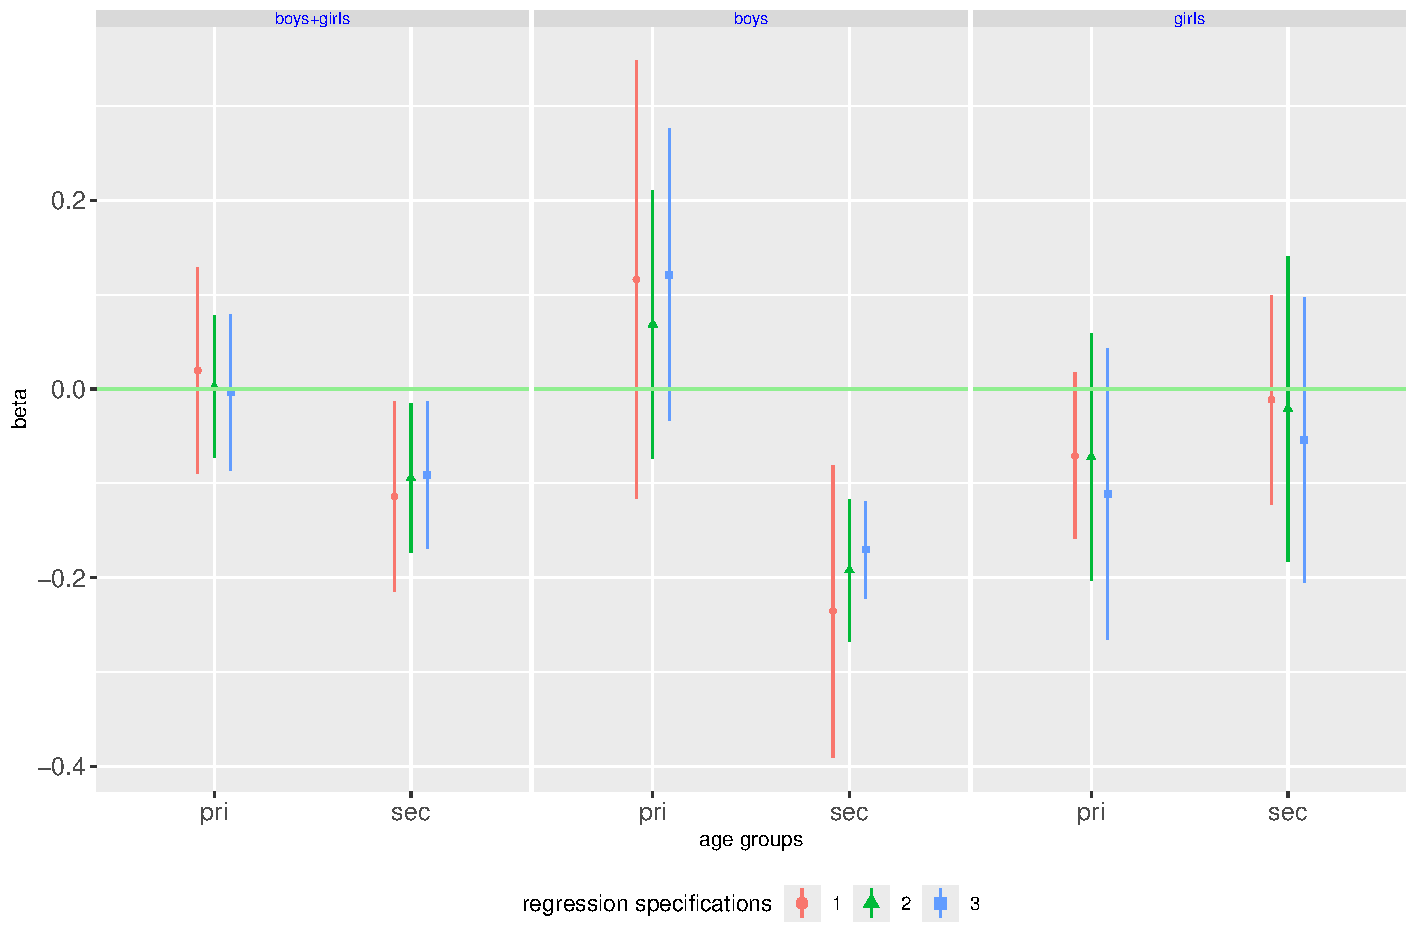
\includegraphics[height=.23\paperheight]{Figures/GenderAgeGroup2Impacts.pdf}\\
\renewcommand{\arraystretch}{1}
\hfil\begin{tabular}{>{\hfill\scriptsize}p{1cm}<{}>{\scriptsize}p{11cm}<{\hfill}}
Source: & Compiled from IFPRI data. \\[-1ex]
Notes:& 1. ``pri'' and ``sec'' mean enrolled in primary and secondary grades, aged 6-10 and 11-17 years in 1999, respectively. The coefficients are dummies for agri-HH $\times$ year 2002.\\[-1ex]
& 2. Specification 1 uses time-varying thana level characteristics (yield, mean rainfall, mean high temperature, mean low temperature), individual-level characteristics (age squared, recipient of a poverty program), and \textsf{demographic fixed trends,} which are the interactions of baseline individual and demographic characteristics (sex of individual, household head's education, number of older male/female siblings) with the year 2002 dummy and the year 2002 * agricultural household dummy. Specification 2 adds \textsf{other household fixed trends} that are the interactions of other baseline household characteristics (per-member land holding, per-member non-land assets, own piped water, and structured toilet). Specification 3 includes \textsf{Thana's fixed trends}. \\[-1ex]
& 3. Error bars are cluster standard errors at thana level with Satterthwaite correction.
\end{tabular}
%\end{minipage}
\end{figure}

\subsection{Placebo tests}

In this sub-section, we conduct placebo tests employing 2002–2006 panel data based on the fact that the 1999 favorable calendar returned to a normal (unfavorable) routine in 2002. Hence, the school enrollment rate should follow the common trend between the treatment and control groups. We test this using two cohorts: 10–18 years old in 1999 (1999 cohort) and 10–18 years old in 2002 (2002 cohort).

%Both cohorts in 2002-2006 panel are not affected, simply because there was no shift in the final exam schedule during this period.\sout{\footnote{Similarly, 6 - 10 years old in 1999 (primary school cohort) may be too young to be affected in 1999. Results of primary school-aged children in \textsc{Table \ref{MainGenderAgeGroup2ResultsWithInteractions}} in Appendix \href{app_a3}{A3} can be seen as placebo test results. }} These cohorts are observed one year after the favorable shifts in the final exam schedules in 1999-2001, and it is unlikely that we continue to observe their impacts in 2002 when there was an exam-harvest overlap.  If this assumption holds, these\sout{ cohorts in 2002-2006 panel are not affected, simply because there was not a shift in the final exam schedule during this period. These} two cohorts present good opportunities to conduct placebo tests for our analysis. 



\begin{table}
\hfil\textsc{\footnotesize Table \refstepcounter{table}\thetable: Placebo test results \label{Placebo10}}\\
\setlength{\tabcolsep}{1pt}
\renewcommand{\arraystretch}{.75}
\hfil\input{Tables/Placebo10AgHHResults.tex}
\renewcommand{\arraystretch}{1}
\hfil\begin{tabular}{>{\hfill\scriptsize}p{1cm}<{}>{\hfill\scriptsize}p{.25cm}<{}>{\scriptsize}p{.7\paperwidth}<{\hfill}}
Notes:& 1. & Sample of direct offspring of household heads. \textsf{Agri HHs * year 2006} is an interaction term of agricultural household dummy and year 2006 dummy. All the interaction terms are demeaned. Columns \textsf{(1) and (4)} use time-varying thana level characteristics (yield, mean rainfall, mean high temperature, mean low temperature) and individual level characteristics (age squared, recipient of a poverty program). \textsf{Demographic fixed trends} are interactions of baseline individual and demographic characteristics (sex of individual, household head's education, number of older male/female siblings) with the year 2002 dummy, and sex of individual with the year 2002 * agricultural household dummy. Parental education is highly collinear with agricultural household dummy and is dropped from triple interactions. Columns \textsf{(2) and (5)} add \textsf{Other household fixed trends} that are interactions of other baseline household characteristics (per member land holding, per member non-land assets, household condition (access water through pipe and having structured toilet at home). Columns \textsf{(3) and (6)} add \textsf{Thana fixed trends}, which allow heterogeneous trends at Thana level. \\[-1ex]
& 2. & Standard errors are clustered at thana level. 95\% confidence intervals of cluster robust standard errors using \cite{liang1986longitudinal} are shown in parenthesis, and bias-reduced linearization (BRL) for a correction of a small number of clusters are shown in square brackets. $*$, $**$, $***$ indicate significance levels at 10\%, 5\%, 1\% under BRL cluster robust standard errors, respectively.
\end{tabular}
\end{table}

Table \ref{Placebo10} provides the results of two sets of placebo tests. All regression specifications follow those of \textsc{Table \ref{base10}}.
%\sout{In column (1), we estimate the equation \eqref{esteqn} with 1999-2002 data for age cut-off of 4-9 year olds in 1999. This age cohort was relatively younger in 1999 and many of them were not even enrolled in school. As a result, this cohort had not benefited much from the favorable examination calendar of 1999. Hence children from agricultural households within this age cohort should not face any differential impact in 2002. As hypothesized, results reported in column (1) show a smaller point estimate with large p-values, supporting our first placebo test.
In Panel A, we report the first placebo test with the same individuals (10-18 years old in 1999) with the later rounds of data. This also provides a validity check for the common trend assumption. Since there was no shift in the academic calendar between 2002 and 2006, we do not expect any differential impact on children from agricultural households in these years. Our coefficient of interest $\hat{\gamma}$ has a smaller point estimate relative to the main results with larger standard errors, leading to large $p$ values.\footnote{The point estimates are all negative, indicating children from agricultural households tend to drop out earlier even when exam-harvest overlap is absent. Consistent with our brawn-based interpretation that female labor is not a perfect substitute for male labor to work in the field, we obtain negative estimates on the triple interaction terms of the number of older female siblings with $p$ values ranging between 7.2\% and 8.9\%. This implies that children from agricultural households are naturally disadvantaged in schooling even if there is no change in exam-harvest overlap when the household demographic structure is unfavorable.}

In the second set of placebo tests, we use 10-18-year-old in 2002 (2002 cohort). The results are provided in Panel B. All the estimates are negative but statistically indistinguishable from zero. The estimation results using the 2002 cohort gender subsamples are presented in \textsc{Table \ref{PlaceboResults10Table}} in Appendix \ref{app_a4}. All of these results show large $p$ values for the impact of the year 2006 interacted with agricultural households, lending support for our identification assumption under the DID setting.

%\begin{table}[h!]
%\caption{\textbf{Placebo Tests 1 with IFPRI Data-set}}
%\label{placebo}
%\begin{center}
%{
%\resizebox{16.5cm}{!}{
%\begin{tabular}{lcccc}
%    \toprule
%\multicolumn{1}{c}{\textbf{Estimations:}} & \multicolumn{1}{c}{\textbf{Placebo Regression 1}} & \multicolumn{2}{c}{\textbf{Placebo Regression 2}} & \multicolumn{1}{c}{\textbf{Placebo Regression 3}}\\
%\cmidrule(lr){1-1}\cmidrule(lr){2-2}\cmidrule(lr){3-4}\cmidrule(lr){5-5}
%\multicolumn{1}{c}{\textbf{Panel-Data:}}       & \multicolumn{1}{c}{\textbf{1999-2002}}& \multicolumn{2}{c}{\textbf{2002-2006}} & \multicolumn{1}{c}{\textbf{2002-2006}} \\
%\cmidrule(lr){1-1}\cmidrule(lr){2-2}\cmidrule(lr){3-4}\cmidrule(lr){5-5}
%\multicolumn{1}{c}{\textbf{Age Cut-off:}}        &  4-9 in 1999    & 10-18 in 2002     & 11-18 in 2002    & 10-18 in 1999        \\
%\cmidrule(lr){1-1}\cmidrule(lr){2-2}\cmidrule(lr){3-4}\cmidrule(lr){5-5}
%\multicolumn{1}{c}{\textbf{Dependent Variable: $\Delta$Enrollment}}  & (1)    & (2)   & (3)   & (4)  \\
%\midrule
%                                                &           &           &           &        \\
%Year 2002 dummy interacted with                 &-0.062     &           &           &        \\
%Agricultural household                          & (0.063)   &           &           &        \\
%                                                &           &           &           &        \\
%Year 2006 dummy interacted with                 &           & -0.010    & -0.008    &  0.027 \\
%Agricultural household                          &           & (0.028)   & (0.017)   &    (0.019) \\
%                                                &           &           &           &               \\
%                                                &           &           &           &                   \\
%\hline
%Other Household level Control                   &    Yes    &  Yes      &   Yes     &   Yes             \\
%Sub-district (Thana) Control                    &    Yes    &  Yes      &   Yes     &   Yes             \\
%\hline
%Number of Observations                          & 265       & 870       & 764       & 635               \\
%R-Square                                        & 0.1047    & 0.1871    & 0.2079    & 0.2553            \\
%\hline
%Mean of control group in 1999                   & 0.897     &           &           &                   \\
%Mean of control group in 2002                   & 0.795     & 0.674     & 0.636     & 0.508                \\
%Mean of control group in 2006                   &           & 0.434     & 0.386     & 0.283                    \\
%\hline\\
%\multicolumn{5}{p{23cm}}{{\footnotesize Source: Compiled from IFPRI data.
%Notes: 1. Regression estimated using a first-difference estimator with standard errors clustered at \textit{thana} level. $*$, $**$, $***$ indicate significance levels at 10\%, 5\%, 1\%, respectively.
%2. Regression estimates control for time variant covariates: \textsf{yield} which represents Thana level paddy yield, \textsf{program} which is an indicator variable if at least one household member receive either safety net or education related program (stipend/scholarship) support, \textsf{mean high temperature} is mean annual temperature of the daily high and \textsf{mean low temperature} is mean annual temperature of the daily low.
%3. Time invariant variables are also interacted with year 1999: \textsf{agricultural household} is an indicator variable for a household whose primary income is agriculture. \textsf{sex (female = 1)} is an indicator variable of child gender. \textsf{head primary, head secondary, spouse primary, spouse secondary} are indicator variables for the respective highest educational achievement. \textsf{per member land holding} is per member land holding of the household in 1999 measured in acres. \textsf{per member non-land asset} is per member non-land asset values in 1999 measured in 1000 BDT. \textsf{own piped water, structured toilet} are indicator variables of household ownership of each facilities. All dummy variables are demeaned. Number of sample is per year cross sectional units. }}
%\end{tabular}}}
%\end{center}
%\end{table}

\subsection{Secondary Outcomes}

In \textsc{\small Table \ref{NumGradesDaysAbsentResults}}, we examine the impacts on secondary outcome related to enrollment continuation: The number of completed grades or grade progression in three years (between 1999-2002),\footnote{Grade progression is defined as the difference in reported grades between 2002 and 1999 for individuals who are not out of school. Out-of-school individuals are those whose schooling is lower than grade 1, who are not enrolled in both 1999 and 2002 rounds, or who are not reporting a change in grade between 1999 and 2002.} and the mean number of days absent from school in the past two months before the survey interview date (July-August 1999 and 2002). Both outcome measures are estimated for those enrolled in 1999 (panel A of Table \ref{NumGradesDaysAbsentResults}) and those enrolled in both the 1999 and 2002 rounds (panel B of Table \ref{NumGradesDaysAbsentResults}). Please note that the sample we used in these exercises is a selected sample containing only regular students; hence, the evidence generated here is suggestive and is likely to provide lower-bound estimates.  

Columns (1)-(3) show the negative impacts on grade progression among children from agricultural households in 2002 when the academic calendar was unfavorable. This negative grade progression estimates range from -0.40 to -0.47 years during 1999-2001 (from the base of 2.37 years of progression by the non-agricultural household children), depending on the specification. In Columns (4)-(6) with the panel B sample, the estimates are similar, however smaller in magnitude, which is reasonable given that the sample used in panel A includes dropouts in 2002 who have fewer grade progressions. This implies that agricultural children plausibly struggle to get ``passing'' scores to continue academic progression, which could be related to inadequate learning owing to school absenteeism, particularly during the peak labor demand season. 

%\SAdded{One should note that this is a cost beyond dropping out: Even if they continue schooling, the grade progression is slower than non-agricultural households.}


 

%In addition, we can also compute the number of grade progression for a larger group of individuals including dropouts as long as they report the highest grades they completed. We call them initial enrollers in panel A of the table.  

%If there is more dropout, the number of grade progression should be less, and the absent days should be greater.

\begin{table}
\hfil\textsc{\footnotesize Table \refstepcounter{table}\thetable: Grade progression and absent days\label{NumGradesDaysAbsentResults}}\\
\setlength{\tabcolsep}{1pt}
\renewcommand{\arraystretch}{.75}
\hfil\input{Tables/NumGradesDaysAbsentResults.tex}
\renewcommand{\arraystretch}{1}
\hfil\begin{tabular}{>{\hfill\scriptsize}p{1cm}<{}>{\hfill\scriptsize}p{.25cm}<{}>{\scriptsize}p{.7\paperwidth}<{\hfill}}
Source:& \multicolumn{2}{l}{\scriptsize Compiled from IFPRI data. }\\[-1ex]
%Notes: &  & Same as Table \ref{base10}. \\
Notes:& 1. & Sample of direct offspring of household heads. \textsf{Agri HHs * year 2002} is an interaction term of agricultural household dummy and year 2002 dummy. All the interaction terms are demeaned. Columns \textsf{(1),(4) and (7)} use time-varying thana level characteristics (yield, mean rainfall, mean high temperature, mean low temperature) and individual level characteristics (age squared, recipient of a poverty program). \textsf{Demographic fixed trends} are interactions of baseline individual and demographic characteristics (sex of individual, household head's education, number of older male/female siblings) with the year 2002 dummy and sex with the year 2002 * agricultural household dummy. Parental education is highly collinear with agricultural household dummy and is dropped from triple interactions. Columns \textsf{(2), (5) and (8)} add \textsf{Other household fixed trends} that are interactions of other baseline household characteristics (per member land holding, per member non-land assets, household condition (access water through pipe and having structured toilet at home). Columns \textsf{(3),(6) and (9)} add \textsf{Thana fixed trends}, which allow heterogeneous trends at the Thana level. Columns (7)-(9) use only 2002 data.\\[-1ex]
& 2. & Standard errors are clustered at thana level. 95\% confidence intervals of cluster robust standard errors using \cite{liang1986longitudinal} are shown in parenthesis, and bias-reduced linearization (BRL) for a correction of a small number of clusters are shown in square brackets. $*$, $**$, $***$ indicate significance levels at 10\%, 5\%, 1\% under BRL cluster robust standard errors, respectively.
\end{tabular}
\end{table}

\subsection{Mechanisms}

In \textsc{\small Table \ref{NumGradesDaysAbsentResults}}, Panel C, we examine the calendar conflict impact on absenteeism outcome as potential impact mechanism. Columns (7)–(9) present the cross-sectional estimates of the impacts on the average monthly absent days for students enrolled in both survey rounds. The sample consists of continuing school students and uses only the year 2002 cross-section. Our estimates indicate that children from agricultural households systematically missed more (about 28\%) school days, on average, during July–August, which overlaps with the local \textit{Aman} paddy plantation time (see section \ref{sec.rice}). Gender sub-sample estimation (not reported but available on request) shows this absenteeism impact predominantly comes from boys. On average, boys from agricultural households missed school about 2.3-2.6 days more per month in 2002 during the plantation time (from the base of 2.5 absent days for non-agriculture household students, an increment equivalent to 92-100\%). 

%Taken together, these results suggest that learning, if measured by regular school attendance, is affected by local agricultural activities. This provides plausible evidence that school absenteeism hinders grade progression and school continuation, particularly when the annual exam is held during the harvesting season.


%This indicates that children of agricultural households drop out more often, and even they decide to stay on school, they lag behind more than non-agricultural household children. This is not surprising. We already knew from the main results that the grade progression should be less for initial enrollers, given this is broadly a flip side of coin of higher dropout rates. However, we could not expect from the main results that the grade progression is slower even among the all time enrollers of agricultural households.


\subsection{Testing for alternative mechanisms}

In Table \ref{FloodNonMuslimResults}, we report two tests to check the plausibility of alternative mechanisms that are consistent with the estimated results: one with non-Muslims and the other with flood\sout{s}-affected areas. 

It is possible that our estimates primarily capture the impact of fasting and festivities during \textit{Ramadan}, which may diminish children’s capacity to learn and pass annual exams. To verify this empirically, we compare Muslim and non-Muslim households. As non-Muslims do not fast and are less prone to be affected by festivities, this exercise helps us disentangle the impact of festivities. Columns (1)–(3) of Table \ref{FloodNonMuslimResults} presents estimates using a non-Muslim dummy and its interaction with the year 2002 and the year 2002*agricultural household. We can observe that our main coefficient of interest does not differ from those in Table \ref{base10}. For non-Muslims, the statistically imprecise point estimates suggest that \textit{Ramadan} before the exam in 2002, fasting before the final exams, and post-\textit{Ramadan} festivities are not plausible mechanisms leading to lower enrollment rates for children from agricultural households.

%However, due to small cell size of non-Muslims, estimates have large standard errors and nothing conclusive can be stated from the results.  

%and we should get statistically significant positive estimates for the interaction term. 


\begin{table}
\hfil\textsc{\footnotesize Table \refstepcounter{table}\thetable: Testing for confounding mechanisms \label{FloodNonMuslimResults}}\\
\setlength{\tabcolsep}{1pt}
\renewcommand{\arraystretch}{.75}
\hfil\input{Tables/FloodNonmuslimResults.tex}

\renewcommand{\arraystretch}{1}
\hfil\begin{tabular}{>{\hfill\scriptsize}p{1cm}<{}>{\hfill\scriptsize}p{.25cm}<{}>{\scriptsize}p{.7\paperwidth}<{\hfill}}
Source:& \multicolumn{2}{l}{\scriptsize Compiled from IFPRI data. }\\[-1ex]
Notes:& 1. & Sample of direct offspring of household heads. Columns \textsf{(1) and (4)} use time-varying thana level characteristics (yield, mean rainfall, mean high temperature, mean low temperature) and individual level characteristics (age squared, recipient of a poverty program). \textsf{Demographic fixed trends} are interactions of baseline individual and demographic characteristics (sex of individual, household head's education, number of older male/female siblings) with the year 2002 dummy, and sex of individual with the year 2002 * agricultural household dummy. Parental education is highly collinear with agricultural household dummy and is dropped from triple interactions. Columns \textsf{(2) and (5)} add \textsf{Other household fixed trends} that are interactions of other baseline household characteristics (per member land holding, per member non-land assets, household condition (access water through pipe and having structured toilet at home). Columns \textsf{(3) and (6)} add \textsf{Thana fixed trends}, which allow heterogeneous trends at Thana level.  \textsf{Flooded} is 1 for Haziganj, Modhupur, Sherpur sadar thanas. Other covariates include interaction terms \textsf{unflooded/nonmuslim * year 2002}. \\[-1ex]
& 2. & Standard errors are clustered at thana level. 95\% confidence intervals of cluster robust standard errors using \cite{liang1986longitudinal} are shown in parenthesis, and bias-reduced linearization (Satterthwaite correction) for a correction of the small number of clusters are shown in square brackets. $*$, $**$, $***$ indicate significance levels at 10\%, 5\%, 1\% under cluster robust standard errors, respectively. 
%N$_{group}$ indicates the number of observations for flooded areas or non-Muslims. 
\end{tabular}
\end{table}

Another possible confounding mechanism that can explain the estimated results is the impact of a natural disaster that systematically affected agricultural households in 2002. If this is true, then our estimates capture the impact of natural disasters on school dropouts. In 2002, several districts were affected by the monsoon flash floods.\footnote{Flood-affected districts were Chandpur, Sherpur and Tangail. To know more about the flood monsoon based flash flood, please check the following website \url{https://reliefweb.int/report/bangladesh/bangladesh-monsoon-floods-2004-post-flood-needs-assessment-summary-report} } Columns (4)-(6) of Table \ref{FloodNonMuslimResults} assess the effects of flooding using a dummy variable of flooded areas and its interaction with the year 2002, and triple interaction with the year 2002 * agricultural household. The triple interaction of flood-affected areas with agricultural households and the year 2002 dummy indicate no statistically discernible impact, suggesting that natural disasters such as floods are not plausible impact mechanisms.

%N$_{ag}$ indicates the number of agricultural households,

%{\color{red}




%We consider this as not direct evidence against our main finding that exam-harvest overlap negatively affects schooling on three grounds. First, we report that raw DID is negative for non-Muslims (X\%) when we expect it to be zero under the null of festivity induced exam failures. Second, the estimated impacts on Muslims remain negative and statistically nonzero. If the impacts we observe are due to fasting and festivity, we should observe their effects on both agricultural and non-agricultural households of Muslims with a similar magnitude, so their estimated impacts should be near zero. Third, the smaller impacts among non Muslims than Muslims mostly reflect a larger drop in enrollment rate among the non-agricultural households of non Muslims. Enrollment rates of agricultural households reduce by almost the same amount between Muslims (-.3204) and non-Muslims (-.3226).  While it is unclear why enrollment rates of non-agricultural households reduce more among non Muslims, results in \textsc{ Table \ref{FloodNonMuslimResults}} are inconsistent with the fasting and festivity mechanism that only affects Muslim households.




%\begin{table}[h!]
%\caption{\textbf{Competing Mechanisms Tests}}
%\label{falsification}
%\begin{center}
%{
%\resizebox{16.5cm}{!}{
%\begin{tabular}{lcccc}
%    \toprule
%\multicolumn{1}{c}{\textbf{Estimations:}}& \multicolumn{2}{c}{\textbf{Regression with non-Muslim}}  & \multicolumn{2}{c}{\textbf{Regression with Flood}}\\
%\cmidrule(lr){1-1}\cmidrule(lr){2-3}\cmidrule(lr){4-5}
%\multicolumn{1}{c}{\textbf{Panel-Data:}}       & \multicolumn{2}{c}{\textbf{1999-2002}}& \multicolumn{2}{c}{\textbf{1999-2002}}  \\
%\cmidrule(lr){1-1}\cmidrule(lr){2-3}\cmidrule(lr){4-5}
%\multicolumn{1}{c}{\textbf{Age Cut-off:}}        & 10-18 in 1999     & 11-18 in 1999    & 10-18 in 1999   & 11-18 in 1999       \\
%\cmidrule(lr){1-1}\cmidrule(lr){2-3}\cmidrule(lr){4-5}
%\multicolumn{1}{c}{\textbf{Dependent Variable: $\Delta$Enrollment}}  & (1)    & (2)   & (3)   & (4)    \\
%    \midrule
%                                                 &           &           &           &                \\
%Year 2002 dummy interacted with                  & -0.071**  & -0.081**  & -0.068**  &   -0.076**   \\
%Agricultural household                           & (0.030)   &(0.034)    & (0.029)   &  (0.034)     \\
%                                                 &           &           &           &              \\
%Year 2002 dummy interacted with                  & -0.083    & -0.079    &           &              \\
%Agricultural and non-Muslim household            & (0.062)   &(0.084)    &           &              \\
%                                                 &           &           &           &              \\
%Year 2002 dummy interacted with                  &   0.087*  & 0.142**   &           &              \\
%Non-Muslim household                             & (0.052)   &(0.070)    &           &              \\
%                                                 &           &           &           &              \\
%Year 2002 dummy interacted with                  &           &           & -0.016    &   -0.016     \\
%Agricultural household in flood affected areas          &           &           & (0.059)   &   (0.043)    \\
%                                                 &           &           &           &              \\
%\hline
%Other Household level Control                   &   Yes     &   Yes     &   Yes     & Yes           \\
%Sub-district (Thana) Control                    &   Yes     &   Yes     &   Yes     & Yes           \\
%\hline
%Number of Observations                          & 682      & 557        & 682       & 557           \\
%R-Square                                        & 0.4463   & 0.4985     & 0.4435    & 0.4914        \\
%\hline
%Mean of control group in 1999                   & 0.73        & 0.69        & 0.73  & 0.69          \\
%Mean of control group in 2002                   & 0.44        & 0.38        & 0.44  & 0.38          \\
%\hline\\
%\multicolumn{5}{p{21cm}}{{\footnotesize Source: Compiled from IFPRI data.
%Notes: 1. Regression estimated using a first-difference estimator with standard errors clustered at \textit{thana} level. $*$, $**$, $***$ indicate significance levels at 10\%, 5\%, 1\%, respectively.
%2. Regression estimates control for time variant covariates: \textsf{yield} which represents Thana level paddy yield, \textsf{program} which is an indicator variable if at least one household member receive either safety net or education related program (stipend/scholarship) support, \textsf{mean high temperature} is mean annual temperature of the daily high and \textsf{mean low temperature} is mean annual temperature of the daily low.
%3. Time invariant variables are also interacted with year 1999: \textsf{agricultural household} is an indicator variable for a household whose primary income is agriculture. \textsf{sex (female = 1)} is an indicator variable of child gender. \textsf{head primary, head secondary, spouse primary, spouse secondary} are indicator variables for the respective highest educational achievement. \textsf{per member land holding} is per member land holding of the household in 1999 measured in acres. \textsf{per member non-land asset} is per member non-land asset values in 1999 measured in 1000 BDT. \textsf{own piped water, structured toilet} are indicator variables of household ownership of each facilities. All dummy variables are demeaned. Number of sample is per year cross sectional units. }}
%\end{tabular}}}
%\end{center}
%\end{table}	


%\subsection{Impact Heterogeneity}

%To understand the impact heterogeneity we additionally performed age-cohort specific heterogeneity estimations which are reported in Table \ref{hetero}. In the first two columns we categorized children into three age groups---age 12-13, 14-15 and 15 and above. In the next two columns, we reclassify the children by making the age-groups 13-15 and 15 and above. In the last two columns we classify age groups based on grade enrollment (primary, secondary or high school). All these age or grade specific dummies are estimated along with the interaction term with the year 2002 and agricultural household dummy. Although we did not report the estimates of the age-cohort dummies for brevity, we see that higher age leads to higher dropout rates, which have low p-values and the impact magnitude is higher for older children. To give a perspective, the school dropout rate jumps from 10pp (for 12-13 years old) to 30pp for 15 and above aged children compared with the default age category. A similar trend is observed for the re-classified age-cohort group --- it varies from 16.6pp (for 13-15 years old) to 29pp for 15 and above aged children, and also for high school enrolled. However inclusion of all these different age-specific cohort dummies and the interaction terms with year 2000 and agricultural household dummies do not alter our main estimate and we do not observe any systematic differential affect between agricultural and non-agricultural household children of different age cohorts. This finding of no age-group wise impact heterogeneity indicates that the favorable shift in the exam schedule have uniformly benefited the children of a wide range of ages, or for all school going ages. 

%\begin{table}[h!]
%\caption{\textbf{Impact Heterogeneity estimates with 10-18 years old}}
%\label{hetero}
%\begin{center}
%{
%\resizebox{16.5cm}{!}{
%\begin{tabular}{lccccccc}
%    \toprule
%\multicolumn{1}{c}{\textbf{Dependent Variable: }} & \multicolumn{2}{c}{\textbf{Age grouping: Main}} & \multicolumn{2}{c}{\textbf{Age grouping: Alternative}}  & \multicolumn{2}{c}{\textbf{Age grouping: Grade}}\\
%\cmidrule(lr){2-3}\cmidrule(lr){4-5}\cmidrule(lr){6-7}
%\multicolumn{1}{c}{\textbf{Change in Enrollment}} & (1)   & (2)   & (3)   & (4)   & (5)   & (6)  \\
%    \midrule
%Year 2002 dummy interacted with                  &            &           &           &           &           &            \\
%Agricultural household                           &-0.070***   &-0.068**   & -0.068**  & -0.068**  & -0.066**  & -0.062**    \\
%                                                 & (0.23)     & (0.026)   & (0.023)   & (0.026)   & (0.025)   &  (0.026)    \\
%Year 2002 dummy interacted with                  &            &           &           &           &           &             \\
%Agricultural household and age 12-13             &  -0.044    &  -0.049   &           &           &           &            \\
%                                                 &  (0.061)   &  (0.061)  &           &           &           &             \\
%Year 2002 dummy interacted with                  &            &           &           &           &           &            \\
%Agricultural household and age 14-15             &  -0.031    &  -0.029   &           &           &           &             \\
%                                                 & (0.077)    & (0.078)   &           &           &           &             \\
%Year 2002 dummy interacted with                  &            &           &           &           &           &            \\
%Agricultural household and age 15 plus           &  -0.004    &  -0.006   &           &           &           &             \\
%                                                 & (0.072)    & (0.072)   &           &           &           &             \\
%Year 2002 dummy interacted with                  &            &           &           &           &           &            \\
%Agricultural household and age 13-15             &            &           & 0.003     &  0.000    &           &            \\
%                                                 &            &           & (0.065)   & (0.066)   &           &             \\
%Year 2002 dummy interacted with                  &            &           &           &           &           &            \\
%Agricultural household and age 15 plus           &            &           & 0.015     &  0.014    &           &             \\
%                                                 &            &           & (0.061)   & (0.062)   &           &             \\
%Year 2002 dummy interacted with                  &            &           &           &           &           &             \\
%Agricultural household and Primary (grade 4-5)         &            &           &           &           &  0.027    &  0.033      \\
%                                                 &            &           &           &           &  (0.044)  & (0.044)     \\
%Year 2002 dummy interacted with                  &            &           &           &           &           &             \\
%Agricultural household and secondary (grade 6-8)       &            &           &           &           &  0.023     &  0.026       \\
%                                                 &            &           &           &           &  (0.138)  & (0.137)     \\
%Year 2002 dummy interacted with                  &            &           &           &           &           &             \\
%Agricultural household and high (grade 9-12)           &            &           &           &           &  -0.035   & -0.035      \\
%                                                 &            &           &           &           &  (0.140)  &  (0.141)    \\
%\hline
%Other Household level Control          &  Yes      &   Yes     &   Yes     &   Yes     &   Yes     &  Yes        \\
%Sub-district (Thana) Control           &  No       &   Yes     &   No      &   Yes     &   No      &  Yes        \\
%\hline
%Number of Observations                 & 682        & 682       & 682      & 682       & 682      & 682            \\
%R-Square                               & 0.4386     & 0.4373    & 0.4454   & 0.4441    & 0.4516   & 0.4504         \\
%\hline
%Mean of control group in 1999         & 0.73        & 0.73      & 0.73      &  0.73     & 0.73     & 0.73          \\
%Mean of control group in 2002         & 0.46        & 0.46      & 0.46      & 0.46      & 0.46     & 0.46          \\
%\hline\\
%\multicolumn{7}{p{22cm}}{{\footnotesize Source: Compiled from IFPRI data. Cohort of 12 - 18 year aged children in 1999.
%Notes: 1. Regression estimated using a first-difference estimator with standard errors clustered at \textit{thana} level. $*$, $**$, $***$ indicate significance levels at 10\%, 5\%, 1\%, respectively.
%2. Regression estimates control for time variant covariates: \textsf{yield} which represents Thana level paddy yield, \textsf{program} which is an indicator variable if at least one household member receive either safety net or education related program (stipend/scholarship) support, \textsf{mean high temperature} is mean annual temperature of the daily high and \textsf{mean low temperature} is mean annual temperature of the daily low.
%3. Time invariant variables are also interacted with year 1999: \textsf{agricultural household} is an indicator variable for a household whose primary income is agriculture. \textsf{sex (female = 1)} is an indicator variable of child gender. \textsf{head primary, head secondary, spouse primary, spouse secondary} are indicator variables for the respective highest educational achievement. \textsf{per member land holding} is per member land holding of the household in 1999 measured in acres. \textsf{per member non-land asset} is per member non-land asset values in 1999 measured in 1000 BDT. \textsf{own piped water, structured toilet} are indicator variables of household ownership of each facilities. All dummy variables are demeaned. Number of sample is per year cross sectional units. }}
%\end{tabular}}}
%\end{center}
%\end{table}

\section{Long-term Cohort analysis in Bangladesh\label{sec.long-term}}


Table \ref{cohort1} reports the estimates of equation \ref{longruneqn} using a cohort analysis. Column (1) of Panel A reports the regression estimates for years of education. We noticed that the rural population had less schooling than the urban counterpart, which is a common trend in developing countries. Nevertheless, the negative effect on Rural children was significantly lessened in the 10-18 cohort relative to the older cohort. Our estimates indicate that holding all other things constant, the urban-rural enrollment gap has shrunk by 0.46 years for the 10-18-year-old cohort of 1999. This impact is sizable and \sout{statistically significant}has a low $p$ value. In Panel B, we disaggregate the age bracket into 10-12, 13-15, and 16-18 years old in 1999. Our estimates are consistent, as shown in Panel A, and the impact is greater for the secondary school age (10-12 and 13-15 years old in 1999) in rural areas. 

%different age-cutoff of 10-36 years old in Table \ref{cohort2}, keeping three cohorts, namely 10-18, 19-27, and 28-36 years old in 1999 in our estimation. Our estimates of Table \ref{cohort2} are strongly consistent with the estimates of Table \ref{cohort1}. In Table \ref{cohort} we further disaggregated the age-bracket of our cohort of interest and employed age-specific estimates using both age cut-offs. Consistent with previous findings, we see the impact is much larger for the youngest one in the cohort and the impact magnitude gradually declines for the older ones within the cohort.

\begin{table}[h!]
\caption{\textbf{Cohort Analysis: Aged 10-27 in 1999}}
\label{cohort1}
\begin{center}
{
\resizebox{12.5cm}{!}{
\begin{tabular}{lcccc}
    \toprule
\textbf{Variables}                          & \textbf{Years of }    & \textbf{Primary}  & \textbf{Secondary}  & \textbf{Higher}  \\
                                            &\textbf{Education}    &                   &                     & \textbf{Secondary} \\
\cmidrule{2-5}
\textbf{Estimation: } & \multicolumn{1}{c}{\textbf{OLS}} & \multicolumn{3}{c}{\textbf{Probit (Marginal Effects)}}\\
\cmidrule(lr){2-2}\cmidrule(lr){3-5}
\multicolumn{1}{c}{}                        & (1)                   & (2)               & (3)                   & (4)          \\
\hline
%{\textbf{Panel A:  }}                        &                       &                   &                       &               \\
%Aged 6-18 in 1999                           &       1.665***        &       0.193***    &       0.121***        &      0.0589***\\
%                                           &    (0.0598)         &   (0.00712)         &   (0.00478)         &   (0.00426)         \\
{\textbf{Panel A:}}                         &                      &               &                            &                    \\
Cohort: Aged 10-18 in 1999                         &       4.278***&       0.396***&       0.366***&       0.317***\\
                                           &     (0.119)         &    (0.0110)         &    (0.0113)         &   (0.00957)         \\
[1em]
(Aged 10-18 in 1999) X (Rural)               &       0.462***&      0.0532***&      0.0531***&      0.0334***\\
                                           &     (0.112)         &    (0.0106)         &    (0.0106)         &   (0.00859)         \\
[1em]
Rural                                      &      -2.155***&      -0.164***&      -0.199***&      -0.160***\\
                                              &     (0.174)         &    (0.0153)         &    (0.0137)         &    (0.0105)         \\
[1em]
{\textbf{Panel B:}}                         &                   &                       &                   &                   \\
Age 10-12 in 1999                            &       4.188***&       0.381***&       0.359***&       0.312***\\
                                            &     (0.137)         &    (0.0136)         &    (0.0116)         &    (0.0103)         \\
[1em]
Age 13-15 in 1999                            &       2.322***&       0.253***&       0.159***&       0.146***\\
                                            &     (0.141)         &    (0.0122)         &    (0.0124)         &    (0.0104)         \\
[1em]
Age 16-18 in 1999                           &       1.414***&      0.0796***&      0.0197         &       0.151***\\
                                            &     (0.135)         &    (0.0140)         &    (0.0136)         &    (0.0118)         \\
[1em]
(Age 10-12 in 1999) X (Rural)               &     0.587***&      0.0718***&      0.0628***&      0.0401***\\
                                            &     (0.139)         &    (0.0141)         &    (0.0118)         &    (0.0103)         \\
[1em]
(Age 13-15 in 1999) X (Rural)              &       0.773***&      0.0825***&      0.0730***&      0.0374***\\
                                            &     (0.141)         &    (0.0139)         &    (0.0135)         &   (0.00981)         \\
[1em]
(Age 16-18 in 1999) X (Rural)               &     -0.0272         &    0.000236         &      0.0185         &      0.0201         \\
                                             &     (0.143)         &    (0.0155)         &    (0.0156)         &    (0.0134)         \\
[1em]
Rural                                      &      -2.155***&      -0.164***&      -0.199***&      -0.160***\\
                                           &     (0.174)         &    (0.0152)         &    (0.0137)         &    (0.0105)         \\
\hline
Mean of older cohort: aged 19-27 in 1999                  &   4.31            &      0.46     &       0.27        &  0.15                         \\
Mean of older sub-cohort: aged 19-21 in 1999                  &   4.61           &      0.50     &       0.29        &  0.15                         \\
Mean of older sub-cohort: aged 22-24 in 1999                  &   4.23           &      0.45     &       0.26        &  0.15                         \\
Mean of older sub-cohort: aged 25-27 in 1999                  &   3.93           &      0.42     &       0.25        &  0.14                         \\
Other Control                               &    Yes    &  Yes      &   Yes     &   Yes       \\
District Control                            &    Yes    &  Yes      &   Yes     &   Yes       \\
District \times \textnormal{Age Control}                            &    Yes    &  Yes      &   Yes     &   Yes       \\
Observations                                &       49165         &       49129         &       49128         &       48987         \\
\hline
\hline\\
\multicolumn{5}{p{15cm}}{{\footnotesize Source: Compiled from the HIES 2016 data.
Notes: 1. Standard errors are clustered at \textit{district} level are reported in parentheses. $*$, $**$, $***$ indicate significance levels at 10\%, 5\%, 1\%, respectively.
2. Regression estimates control for cohort of birth dummy, sex, district and cohort of birth dummy interactions, and religion.}}.
\end{tabular}}}
\end{center}
\end{table}


Columns (2)–(4) provide the estimates of the probit regression for different stages of academic qualification, namely Primary, Secondary, and Higher Secondary. Our estimates indicate that the probability of completing primary, secondary, and higher secondary education increased by approximately 5.3, 5.3, and 3.4 percentage points, respectively, for the 10–18-year-old rural cohort in 1999 compared to the base. In Panel B, we similarly disaggregate the age brackets and, consistent with the previous finding, observe that secondary school-aged children benefited the most from this exogenous shift in the examination calendar. To test the robustness of our analysis, we use age-specific interaction with rural dummies, which are reported in Table \ref{cohort2} in Appendix \ref{app_a4}. As we can see from Table \ref{cohort2} the impact is predominantly limited to 10-15 years of age in 1999, who got the full impact exposure of the academic calendar shift. Older students also benefited, however, only partially and limited to higher secondary completion, as expected. 

To understand the economic return of this impact, we estimate the private return of education by employing Mincer's (1974) regression following Montenegro and Patrinos (2014). We utilize HIES 2016 data for this estimation (reported in Table \ref{mincer} in Appendix \ref{app_a4}). Based on this framework, we regress the natural logarithm of annual wage earnings on years of education, age, age squared, sex, location (rural or urban), and regional dummies (district level) with standard errors clustered at the district level.\footnote{The regression specification used for individual $i$ in district $j$ is the following: $Log(Income)_{i,j}=\beta_{1}Education_{i,j}+\beta_{2}Age_{i,j}+\beta_{3}Age^{2}_{i,j}+\beta_{4}Male_{i,j}+\beta_{5}Urban_{i}+\delta_{j}+e_{i,j}$.}
We find that the economic return from an additional year of education is approximately 6.6 percent. This is consistent with \cite{montenegro2014comparable} estimates on Bangladesh, which reported an internal rate of return of 5.9 (using estimates of the year 2000) for each additional year of schooling. 

Plugging our cohort estimates into the education rate of return calculation indicates that shifting the academic calendar in favor of agricultural households led to an increase of about 3.03 percent in wages (or 2.71 percent if we use \cite{montenegro2014comparable} estimate). This estimated economic return is comparable to other education-related interventions, such as the Conditional Cash Transfer (CCT) program in Mexico.


\section{Estimates using India sample}

As mentioned in the introduction, the impact of the seasonal agricultural harvesting period overlapping with the school academic session (particularly the grade completing exam) is an issue faced by several developing countries, particularly agriculture-dominated ones. To check the cogency of this claim, one can conduct an exercise with data from other countries with similar settings. One promising country to conduct such an analysis is India, a country neighboring Bangladesh, where agriculture is the dominant economic sector. Like Bangladesh, India also faces large school dropout rates.

In India, the state-supported public school system is the primary education provider. These state-supported schools are governed by state-level academic calendars in which some states follow academic sessions from January to December, similar to Bangladesh. However, most states follow different academic calendars depending on their locality, history, and climatic conditions (e.g., monsoon). Consequently, the academic calendars of most states, particularly the timing of annual exams, overlap with those of the primary crop-harvesting period. 

Consider \textit{Madhya Pradesh} as an example, where wheat is the dominant crop of the state. The final examination of the public schools in \textit{Madhya Pradesh} is in March, which overlaps with the wheat harvesting season between February and April. However, several states, such as \textit{Bihar}, experience no such overlap since the dominant crop of the state is rice, which is harvested between September and November, whereas the final examinations are scheduled for March. Hence, we can utilize state-wise academic calendar variations to detect the impact of such an overlap on school continuation for children from agricultural households. This impact mechanism is slightly different from that of the Bangladesh setting, as it tests the cumulative effect of overlapping with examinations on educational attainment, not the one-time impact of the exam shift. However, one should note that this analysis may be non-causal as it requires strong assumptions that the state-level placement of school calendars in India is quasi-random. Nevertheless, the following India analysis provides more suggestive evidence for the external validity of the Bangladesh findings. 

To do this analysis, we first generate Table \ref{india3} of the Appendix, where we report state-specific dominant crops and their harvesting seasons for India, coupled with school academic sessions, final exam timing, and whether there is an overlap with the harvesting and academic calendar.\footnote{We could not use Chandigarh and Sikkim in our analysis due to data limitation.} In Table \ref{india3}, state-wise agricultural information is obtained from Government of India \citep{doac2017agricultural} while academic session information has been taken from the \cite{doac2011education}. Second, we employ the panel version of the Indian Human Development Survey (IHDS) data collected in 2004-05 and 2011-12.\footnote{IHDS-1 interviewed 41,554 households (215,774 individuals) in 1503 villages and 971 urban neighborhoods across India. The second phase of the survey re-interviewed most of the households (N=42152) in 2011-12. To link the dataset from both rounds, we follow the instructions given on the IHDS website.} We begin with those interviewed in both rounds of IHDS (N=150,988) to form the balanced panel. Unlike most education surveys, the IHDS collects information on a range of variables, such as details on children's education, landholding, employment, and economic status. To aid our analysis, we merge other variables, such as rainfall, the area under crops, and major cereal production, with the IHDS data. We obtained state-wise rainfall and cereal production information from the Indian Meteorological Department (IMD) and the Directorate of Economics and Statistics, Government of India (GoI), respectively.

For our analysis, we consider only those children who enrolled in school during the first round of the IHDS survey and were within the age range of 6-14 (and also 5-13 years for robustness checks).\footnote{Unlike Bangladesh analysis, we could not use age 10-18 as our age cutoff given the difference between the two survey waves is seven years. According to the Eighty-Sixth Amendment Act (2002), the constitution of India provides free and compulsory education to all children in the age group of six to 14 years as a fundamental right.} To identify agricultural households, we generate an agriculture dummy that takes the value of one if the household head is employed in the agricultural sector during the baseline, as classified in the IHDS survey.  We defined an ``overlap-state'' dummy where the harvesting time of the major crop overlaps with the annual school final exam based on Table \ref{india3} in Appendix A3.\footnote{One caveat is \textit{Kerala} where the major crop is rubber, which does not have a harvesting season in the conventional sense; hence we have taken rice (the second largest crop) as the representative crop for the state.} We consider only the harvesting period of the dominant crop produced in the state, defined by the maximum share of the gross cropped area allotted to that crop. Information on the academic sessions in different states is gathered from the Ministry of Human Resource Development of the GoI. Table \ref{tab_destat_5} in Appendix A3 presents the descriptive statistics of the Indian sample in our study.

We estimate the impact of the state-specific overlapping calendar on school continuation using triple-difference regressions, in which one difference is taken between agricultural and non-agricultural households, one between overlapping and non-overlapping states, and the other between the two survey rounds. Here, the household type and overlapping state dummies are time-invariant by definition.

Specifically, we use a triple-difference specification where ${Enroll}_{iht}$ is a binary variable indicating enrollment status for individual $i$, located in household $h$ in period $t$. Similarly, ${YrEdu}_{iht}$ captures completed years of education for an individual $i$, in household $h$ in period $t$. ${X}_{iht}$ are covariates and ${Year2011}_{iht}$ is the Year 2011 dummy. We estimate the following two equations as fixed-effect estimators with household fixed effect, where $\varepsilon$ is the error term clustered at the household level. Our main coefficient of interest is $a_4$ which estimates the triple difference variable of $\textnormal\symup{Year2011}_{iht}\times \textnormal{Overlapping-State}_{ih}\times\textnormal{Agri}_{ih}$ in both equations \ref{diff_enroll} and \ref{diff_edu} are given below.

%\symup\Delta ${A}_{i,h,t}$ denotes $A_{i,h,t} - \bar{A}_{ih}$ where $\bar{A}_{ih} = {T}^{-1}\sum_{t=1}^{T}A_{i,h,t}$.
\begin{eqnarray}
	\textnormal\symup {Enroll}_{iht} & = &
    a_1 \textnormal\symup {Year2011}_{iht}
    + a_2 \textnormal\symup {Year2011}_{iht}\times\textnormal{Agri}_{ih} \nonumber\\
    &+& a_3 \textnormal\symup  \textnormal{Year2011}_{iht}\times\textnormal{Overlapping-State}_{ih} \nonumber\\
    &+& a_4 \textnormal\symup {Year2011}_{iht}\times \textnormal{Overlapping-State}_{ih}\times\textnormal{Agri}_{ih}   \nonumber \\
    &+& a_5\textnormal\symup {X}_{iht} + \symup\varepsilon_{ht}, \label{diff_enroll}
\end{eqnarray}
\begin{eqnarray}
	\textnormal\symup {YrEdu}_{iht} & = &
    a_1 \textnormal\symup {Year2011}_{iht}
    + a_2 \textnormal\symup {Year2011}_{iht}\times\textnormal{Agri}_{ih} \nonumber\\
    &+& a_3 \textnormal\symup  \textnormal{Year2011}_{iht}\times\textnormal{Overlapping-State}_{ih} \nonumber\\
    &+& a_4 \textnormal\symup {Year2011}_{iht}\times \textnormal{Overlapping-State}_{ih}\times\textnormal{Agri}_{ih}   \nonumber \\
    &+& a_5\textnormal\symup {X}_{iht} + \symup\varepsilon_{ht}. \label{diff_edu}
\end{eqnarray}


 

\begin{table}[h!]
\caption{\textbf{Estimates with India Data}}
\label{india1}
\begin{center}
{
\resizebox{16.5cm}{!}{
\begin{tabular}{lcccc}
    \toprule
\multicolumn{1}{c}{\textbf{Dependent Variable: }} & \multicolumn{2}{c}{\textbf{Enrollment}} & \multicolumn{2}{c}{\textbf{Years of Education}}\\
\cmidrule(lr){2-3}\cmidrule(lr){4-5}
\multicolumn{1}{c}{\textbf{Age group:}} & \multicolumn{1}{c}{\textbf{5-13 in 2004}} & \multicolumn{1}{c}{\textbf{6-14 in 2004}} & \multicolumn{1}{c}{\textbf{5-13 in 2004}} & \multicolumn{1}{c}{\textbf{6-14 in 2004}}\\
\cmidrule(lr){2-2}\cmidrule(lr){3-3}\cmidrule(lr){4-4}\cmidrule(lr){5-5}
                                        & (1)               & (2)           & (3)               & (4)           \\
 \midrule
Year 2011                               &       -0.131*** &       -0.139*** &        4.018*** &        3.878*** \\
                                        &    (-0.0322)      &    (-0.0315) &     (-0.156)       &     (-0.157) \\
(Agri) X (Yr 2011)                      &      -0.0456*** &      -0.0558*** &     -0.106 &       -0.144**  \\
                                        &    (-0.0133)      &    (-0.0136) &    (-0.0672) &    (-0.0669) \\
(Overlapping state) X (Yr 2011)         &    -0.0236 &      -0.0283*   &      0.113 &     0.0678 \\
                                        &    (-0.0152) &    (-0.0157) &     (-0.083) &    (-0.0825) \\
(Overlapping state) X (Agri) X (Yr 2011) &      -0.0655*** &    -0.0543** &       -0.214*   &       -0.221*   \\
                                        &     (-0.022) &    (-0.0225) &     (-0.113) &     (-0.113) \\
\hline
Other Household level Control            &    Yes      &   Yes         &    Yes      &   Yes         \\
District Control                         &   Yes       &   Yes         &   Yes       &   Yes         \\
\hline
Observations         &      18922 &      19184 &      18922 &      19184 \\
R-Square (within)    &      0.428 &      0.452 &       0.86 &      0.856 \\
Mean of control group in 2011          &       0.72 &       0.69 &          8 &       8.24 \\
\hline\\
\multicolumn{5}{p{20cm}}{{\footnotesize Source: Compiled from IHDS 2004-05 and 2011-12 data.
Notes: 1. Regression estimated using a panel fixed effect estimator with standard errors clustered at the household level.. $*$, $**$, $***$ indicate significance levels at 10\%, 5\%, 1\%, respectively.
2. We used the nuclear households. The regression estimates control for time-variant covariates: Age, age squared, parents’ age, education, and the number of household assets. We also control for major state-level crop yields, agricultural areas, and rainfall. 
3. Time-invariant variables interact with the year 2011. An agricultural household is an indicator variable for a household whose primary occupation is agriculture. Overlapping State is an indicator variable of the states in which the major harvesting crop of the state overlaps with the schools’ annual exam period. }}
\end{tabular}}}
\end{center}
\end{table}

%\begin{table}[bp]
%\caption{\textbf{Years of education estimates in India}}
%\label{india2}
%\begin{center}
%{
%\resizebox{16.5cm}{!}{
%\begin{tabular}{lcccccc}
%    \toprule
% & \multicolumn{3}{c}{\textbf{Age grouping: 5-13 in 2004}} & \multicolumn{3}{c}{\textbf{Age grouping: 6-14 in 2004}} \\
%\cmidrule(lr){2-4}\cmidrule(lr){5-7}\cmidrule(lr){6-7}
%\multicolumn{1}{c}{\textbf{Dependent Variable: }} & \multicolumn{2}{c}{\textbf{Any members}} & \multicolumn{1}{c}{\textbf{Nuclear Member}} & \multicolumn{2}{c}{\textbf{Any members}} & \multicolumn{1}{c}{\textbf{Nuclear Member}}\\
%$\cmidrule(lr){2-3}\cmidrule(lr){4-4}\cmidrule(lr){5-6}\cmidrule(lr){7-7}
%\multicolumn{1}{c}{\textbf{Years of Education}} & (1)   & (2)   & (3)   & (4)   & (5)   & (6)  \\
%    \midrule
%Year 2011              &       5.309***&       3.864***&       4.018***&       5.220***&       3.697***&       3.878***\\
%                    &    (0.0379)         &     (0.141)         &     (0.156)         &    (0.0387)         &     (0.145)         &     (0.157)         \\
%[1em]
%(Agri) X (Yr 2011)         &     -0.0129         &     -0.0991*  &      -0.106         &     -0.0564         &      -0.138** &      -0.144** \\
%                    &    (0.0588)         &    (0.0597)         &    (0.0672)         &    (0.0601)         &    (0.0600)         &    (0.0669)         \\
%[1em]
%(Overlapping state) X (Yr 2011)    &      -0.247***&       0.131*  &       0.113         &      -0.201***&      0.0696         &      0.0678         \\
%                    &    (0.0616)         &    (0.0752)         &    (0.0830)         &    (0.0618)         &    (0.0751)         &    (0.0825)         \\
%[1em]
%(Overlapping state) X (Agri) X (Yr 2011) &  -0.228** &  -0.206** &      -0.214*  &      -0.230** &      -0.206** &      -0.221*  \\
%                    &     (0.101)         &     (0.101)         &     (0.113)         &     (0.102)         &     (0.102)         &     (0.113)         \\
%\hline
%Other Household level Control           &  No      &   Yes     &   Yes     &   No     &   Yes     &  Yes        \\
%District Control                        &  No       &   Yes     &  Yes      &  No     &   Yes      &  Yes        \\
%Observations        &       24378         &       22838         &       18922         &       24584         &       23014         &       19184         \\
%R-Square (within)   &       0.848     & 0.866    & 0.86   & 0.834    & 0.861   & 0.856         \\
%\hline
%Mean of control group in 1999         & 0.73        & 0.73      & 0.73      &  0.73     & 0.73     & 0.73          \\
%Mean of control group in 2011         & 8.00        & 8.00      & 8.00      & 8.24      & 8.24     & 8.24          \\
%\hline\\
%\multicolumn{7}{p{25cm}}{{\footnotesize Source: Compiled from IHDS 2004-05 and 2011-12 data.
%Notes: 1. Regression estimated using a panel fixed effect estimator with standard errors clustered at the household level.. $*$, $**$, $***$ indicate significance levels at 10\%, 5\%, 1\%, respectively.
%2. The regression estimates control for time-variant covariates: Age, age squared, parents’ age, education, and number of household assets. We also control for major state-level crop yields, agricultural areas, and rainfall. 
%3. Time-invariant variables interact with the year 2011. An agricultural household is an indicator variable for a household whose primary occupation is agriculture. Overlapping State is an indicator variable of the states in which the major harvesting crop of the state overlaps with the schools’ annual exam period. }}
%\end{tabular}}}
%\end{center}
%\end{table}

Table \ref{india1} represents the regression estimates based on Equation \ref{diff_enroll}. Column (1) reports the estimates of the triple-difference estimator for enrollment with 5-13 years old in 2004. As we can observe, the 2011 dummy and agricultural household interaction with the 2011 dummy indicates negative impacts on enrollment, demonstrating the natural dropout trend and vulnerability of poor agricultural household students.

After controlling for these effects, we see a sizable negative impact on enrollment in 2011 for agricultural household children who were in schools in the overlapping states relative to agricultural households in non-overlapping states or non-agricultural households in overlapping states. This impact is \sout{highly statistically significant}\SAdded{estimated precisely}, causing about a 6.55 percent decline in enrollment from the mean. We use a different age bandwidth (age 6-14 years old in 2004) in columns (2) of Table \ref{india1}, which show similar estimates. Given India's population, this estimate is sizable, causing millions of children to discontinue their schooling due to the academic calendar conflicting with the local agricultural cycle.  

Columns (3) and (4) of Table \ref{india1} present the estimates of equation \ref{diff_edu} with years of education as a dependent variable and find similar negative impacts, about 0.20 to 0.22 years of fewer schooling between surveys for agricultural households in overlapping states relative to agricultural households in non-overlapping states or non-agricultural households in overlapping states --- supporting our findings with Bangladesh data. However, caution should be exercised in interpreting these results as we do not know the final years of school attainment; these students may be in school at the time of the survey (and students who lag behind may also be able to catch up with time).


\section{Conclusion}

%Our findings suggest that policymakers in agrarian economies may need to revise the school calendar and curriculum to accommodate local labor demand seasonality to minimize its potential adverse effects on school attendance, learning, and continuation. Such a revision would complement demand-side policies in addressing the trade-offs faced by students explicitly. 

Seasonality in agrarian societies is an important issue that must be addressed appropriately to formulate effective public policies. Surprisingly, seasonally adjusted policies outside the context of food security and disaster management are rare. Educational reforms in developing countries often focus on teacher incentives, technology adoption, and better curriculum design; however, the adjustment of the academic calendar has not received due attention. This issue is becoming increasingly important as developing countries aim for greater outreach of universal education and education-related Sustainable Development Goals (SDGs), which require precise targeting for rural school-going children.

This study addresses the impact of seasonal labor demand on school continuation in South Asia. The school calendars for both primary and secondary schools in Bangladesh are not seasonally adjusted for local agricultural cycles, whereas in India, some state school calendars are not designed to accommodate the primary crop harvesting period. We empirically assessed the impact of such overlaps between school exams and harvest periods using a panel data from rural Bangladesh. Our estimates indicate that children from agricultural households benefited significantly from school continuation owing to a favorable off-harvest exam schedule in Bangladesh. In other words, a favorable annual examination schedule away from the harvest season helped school children from agricultural households continue their schooling in 1999. However, there was a substantial decline in enrollment due to the typical unfavorable examination schedule that overlaps with harvesting, which was observed in 2002. Exploiting state-level academic calendar variations, we conducted a complementary analysis of school-enrolled children in India and found supporting evidence on this issue.

Employing a nationally representative household survey, we estimated that this temporary favorable shift in the exam calendar for the 10-18-year-old rural cohort increased years of education by 0.46 years in Bangladesh. Moreover, these additional years of education have a substantial economic return of a 3 percent increase in income. To benchmark this effect, the pioneering CCT program of Mexico, ``Progresa-Oportunidades'' yielded 0.66 additional years of schooling for every eight years of participation in the program \citep{reimers2006education}, while our favorable calendar shift continued for three years. Infrastructural interventions such as large-scale school construction programs in Indonesia yielded an increase of 0.12-0.19 years of education and 3 to 5.4 percent economic return \citep{duflo2001schooling}. Compared to these interventions, fixing the academic calendar to avoid seasonal labor demand appears to be a cost-effective intervention with a sizable return.

Beyond seasonality, ample factors hamper education performance in developing countries. However, adjusting school calendars to accommodate local agrarian calendars can reduce the dilemma faced by children from agricultural households. Moreover, such an adjustment involves a relatively small one-off cost for the curriculum change. The United Kingdom implemented a seasonally adjusted school calendar during World War II, and the impacts were favorable, although the results were anecdotal \citep[][190-191]{Moore2004}. In early 20th-century Japan, the school calendar was adjusted to accommodate daytime work hours, and some students were allowed to attend night school or take shorter courses \citep[][Chapter 3]{JICA2004}. Even in Bangladesh, non-formal education providers, primarily non-governmental organizations (NGOs), have taken necessary steps to adjust school calendars according to seasonality. For instance, schools run by BRAC, a leading NGO, have begun to use a seasonally adjusted school calendar for non-formal education in Bangladesh.

One can reasonably argue that providing a well-targeted subsidy akin to the CCT is a way to achieve the goal of retaining children from agricultural households in schools. Policymakers may also consider alternative measures, such as targeted CCT during the peak labor demand season, to reduce the pull factor for children from poor agricultural households. However, we argue that a school calendar adjusted for local economic activities is advisable as a policy suggestion for two important reasons. First, children’s time use is never dichotomous of schooling or working; on the contrary, a substantial number of children are required to do both, at least in periods of rising seasonal labor demand, such as during harvesting. This reflects the fact that eliminating profitable activities may be costly. Second, adjusting the school calendar to accommodate seasonality is a relatively less expensive and easier administrative solution than providing a well-targeted subsidy. Given these considerations, we expect the results of our empirical analysis to provide a foundation for school calendar reforms that benefit children in agrarian economies, such as Bangladesh, India, and other countries globally.




\pagebreak

\doublespacing
\bibliographystyle{ecta}
\bibliography{ramadan.bib}

\pagebreak
\renewcommand{\thefigure}{A\arabic{figure}}
\renewcommand{\theHfigure}{A\arabic{figure}}
\setcounter{figure}{0}

\renewcommand{\thetable}{A\arabic{table}}
\renewcommand{\theHtable}{A\arabic{table}}
\setcounter{table}{0}

\appendix
\setcounter{secnumdepth}{1}
%\section{Appendix}
\setcounter{section}{0}
\renewcommand{\thesection}{A\arabic{section}}


\section{Theoretical Framework}\label{app_a1}
\setcounter{equation}{0}
%\setcounter{table}{0}
%\setcounter{figure}{0}
\renewcommand{\theequation}{A\arabic{equation}}
%\renewcommand{\thetable}{\Alph{section}\arabic{table}}
%\renewcommand{\thefigure}{\Alph{section}\arabic{figure}}
\newcommand{\defeq}{\mathrel{\mathop:}=}
\newcommand{\bfbeta}{\ensuremath{\mbox{\boldmath $\beta$}}}
\newcommand{\bfgamma}{\ensuremath{\mbox{\boldmath $\gamma$}}}
\newcommand{\bfomega}{\ensuremath{\mbox{\boldmath $\omega$}}}
\newcommand{\bfc}{\ensuremath{\mbox{\boldmath $c$}}}
\newcommand{\bfm}{\ensuremath{\mbox{\boldmath $m$}}}

In this section, we use \cite{BalandRobinson2000} to show a simple theoretical framework to better our understanding of the impact of seasonal labor demand coinciding with the examination period. Consider an individual living over two periods. In the first period, she faces a trade-off between the optimal schooling hours $l$, and work $1-l$. If she chooses school for $l$ hours, she receives an income according to the production function $h(1-l)$, and her second-period income $y$ increases at rate $e(l)>0$ with $e(0) = 1$. We let a multiplicative term $1+aD$ where $a>0$ measure the productivity change in production. In harvest seasons, $D$ takes the value of $1$, and $0$ otherwise for agricultural households. Rewriting $1+aD = m$, the individual's problem is as follows:

\begin{equation}
\begin{aligned}
& \underset{c_{1}, c_{2}, l}{\text{maximize}}
& &  u(c_{1}) + \beta u(c_{2}) \\
& \text{subject to}
& & mh(1-l)=c_{1}+s, and \\
& & & e(l)y+Rs= c_{2},
\end{aligned}
\label{umax}
\end{equation}
where we denoted $c_{t}$ as period $t$ consumption with $t=1,2$, $\beta\in(0, 1]$ as a discount factor, $s$ as savings, $y$ as second-period base income, and $R>0$ as an interest rate factor. Upon substitution, this is equivalent to the following:
\[
\max_{\{s, l\}} u[mh(1-l) - s] + \beta u[e(l)y+Rs].
\]
First-order conditions (FOCs) are as follows, assuming positive savings \footnote{Alternatively, one can assume that the interest rate is an effective interest rate that varies according to household wealth and other entitlements.}
\[
\begin{aligned}
-u'(c_{1})+\beta R u'(c_{2}) &= 0, and \\
-mh'(1-l)u'(c_{1})+\beta e'(l)y u'(c_{2}) &= 0.
\end{aligned}
\]
The second FOC suggests that individuals equate marginal utility loss of income due to schooling in the first period to marginal utility gain due to increased income in the second period. Substituting the first FOC to the second FOC, we have the following:
\begin{equation}
e'(l)  = \tfrac{R}{y}mh'(1-l).
\label{l}
\end{equation}
If there is a uniform market wage rate $w$, then at the equilibrium without any factor market imperfection, we must have $w=mh'(1-l)$. Then the above becomes
\begin{equation}
e'(l)  = \tfrac{R}{y}w.
\label{l'}
\end{equation}
Let us assume that the return to schooling $e$ and production $h$ are strictly concave functions. In addition, assume that regularity conditions $\lim\limits_{l\rightarrow 0}e'(l) = \infty$ and $\lim\limits_{l\rightarrow 0}h'(1-l) = \bar{h}>0$ hold.\footnote{These assure that $l^{*}>0$ to exists. Given that almost everyone attends school to some level and that the Government of Bangladesh introduced compulsory primary education in 1991, these conditions are an effective description of reality.} There exists $l^{*}>0$ that satisfy FOCs, because the left-hand side of \eqref{l} is increasing while the right-hand side is decreasing in $l$. When $D=1$, time of harvesting (and $m>1$), the marginal productivity of labor increases, and $l^{*}$ decreases.

We can alternatively rewrite \eqref{l} as
\begin{equation}
\begin{aligned}
g(l)    &=\frac{R}{y}m, \\
g(l)    &\defeq \frac{e'(l)}{h'(1-l)}, where \ g'<0.
\end{aligned}
\label{gl}
\end{equation}

Taking an inverse function of $\frac{e'}{h'}$, we see that $g(\cdot)$ is nonlinear in $l$. We approximate \eqref{gl} by log-linearization:
\[
 l_{i,t}\backsimeq  l^{*}_{i}+\tilde{a}\{(\ln R_{t}-\ln R^{*}_{i}) - (\ln y-\ln y^{*}_{i}) + (\ln m_{t}-\ln m^{*})\} + v_{i},
\]


where $\tilde{a}=\tfrac{R^{*}_{i}m^{*}}{g''(l^{*})y^{*}}$ and $v_{i}=-\tfrac{g'(l^{*}_{i})}{g''(l^{*}_{i})}$. Noting that $y$ is second-period base income and $R_{t}$ is the person-specific interest rate, these are functions of household and individual characteristics $\textbf{x}_{i,t}$ with $R_{t}=R(\textbf{x}_{i,t})$ and $y=y(\textbf{x}_{i,t})$. Further approximating these functions will give a linear equation in $\textbf{x}_{i,t}$. Hence, we arrive at,

\begin{equation}
 l_{i,t}- l^{*}_{i}\backsimeq \bfbeta'(\ln \textbf{x}_{i,t}-\ln \textbf{x}^{*}_{i}) + \gamma(\ln m_{t}-\ln m^{*}) + v_{i},
 \label{lsimeq}
\end{equation}
which provides the basis for the estimating equation \eqref{estbase} in Section \ref{sec.id}.

Passing the examination and continuing schooling are critical for students to achieve greater human capital for a future increase in income. The impact of having the annual final examination during the off-peak seasonal labor demand period is equivalent to a decrease in productivity or wage rates in this model. In Bangladesh in 1999, \textit{Ramadan} school holidays resulted in the rescheduling of the annual final exam of schools to the pre-harvest period. Hence, individuals faced a lower marginal labor productivity or wage during the examination period of 1999 than in any typical year. This can be expressed as having a lower value for $m$. Comparing the favorable final exam schedule of 1999 with the unfavorable one of 2002 -- between agricultural and non-agricultural will enable us to identify its impact on enrollment.

% In 1999, lower labor demand during the exam period allowed individuals to concentrate on preparing for examinations or to choose a larger $l^{*}$

\pagebreak

\section{Explanations of DID Framework}\label{app_a2}

The reverse time order of policy and observation requires an additional assumption from regular DID specification. In addition to the common (parallel) trend in the absence of an exam schedule shift, one needs the impact to be one-time and tapering off by the second period. \textsc{\small Figure \ref{ididea}} graphically illustrates these two assumptions (and Figure \ref{ptrendDHS} shows empirically with the DHS data). For the ease of exposition, we include the before-baseline period $t_{0}$. The \textit{Ramadan} favorable examination schedule happens in the period of $t_{1}$ and disappears in period $t_{2}$. In the absence of this exogenous shift in exam schedule at period $t_{1}$, both agricultural and non-agricultural households should have shared a common trend (depicted with dotted gray lines in Figure \ref{ididea}). With the aid of a favorable exam calendar in $t_{1}$, the observed enrollment rate of agricultural households (depicted with the first blue point of $s^{A}$ in Figure \ref{ididea}) is higher than the counterfactual. However, once it reaches period $t_{2}$, with the typical concurrence of the final examination coinciding with the harvest season, we see a disproportionate decrease in the enrollment rate for students in agricultural households relative to students in non-agricultural households. This disproportionate decrease is what we aim to estimate as the impact of an unfavorable examination calendar that coincides with peak harvest season.

\begin{figure}[h!]
\centering
\includegraphics[width = 8.5cm, height = 9cm]{Figures/Framework2.jpg}\\
\caption{Graphical illustration of identification.\footnote{In the diagram $s$ denotes the enrollment rate and $t$ denotes time. Gray points are not observed but assumed. Blue points are observed in our research design. We assume a common trend in the absence of \textit{Ramadan} induced school holidays, and its impacts keep students at school in $t_{1}$ who would have otherwise dropped out. Such favorable impact dissipates in $t_{2}$.}}
\label{ididea}
\end{figure}



One may feel that the one-off impact assumption is too strong. However, this can be justified under a rational schooling decision. If the schooling demand is rational, in the sense that it is optimal given the current conditions and future prospects, then, \textit{cetris paribus}, a student at the margin who stayed in school because the marginal product of labor (MPL) was lower due to no exam-harvest overlap, will drop out in the next period once the MPL increases under exam-harvest overlap. In the absence of any additional schooling policy to improve enrollment (such that it reduces the opportunity cost of schooling), rational students will discontinue schooling, which makes the impact one-off. 

The impacts may last more than one period under certain scenarios. The first is when the students are irrational. If they are irrational in the sense that they change their decision rule and continue enrollment just because they unexpectedly benefited from schooling. In that case, even if the MPL increases to the level under exam-harvest overlap, as in the case of sunk cost fallacy, the impacts last more than one period. Second is enrollment rate-based policy placement. As exemplified in the above, if policymakers target high enrollment areas to reduce schooling costs, it will induce longer-lasting enrollment rate hikes. 

We remain agnostic about the extent to which these two scenarios hold in practice. We also note that longer-lasting impacts can give underestimated impacts. If the impact remains indefinitely, the estimate will be zero because both the treated and the control will follow the common trend. This implies that the impacts will likely be underestimated to the extent that the one-off impact assumption does not hold. In light of this, our estimate potentially gives attenuated impacts if this additional assumption does not hold.

%One may feel that the one-time impact assumption is too strong to be justified. One can rationalize this by reinterpreting the estimates in the spirit of local average treatment effect (LATE) estimates. If we consider the interaction of the natural experiment and agricultural household dummy as an instrumental variable, then the estimated impacts are defined on the subpopulation of agricultural households that discontinues schooling when exam and seasonal labor demand coincide. This subpopulation of agricultural households will discontinue schooling as soon as the favorable examination schedule ends, so one can consider the impacts to be a one-time event. Rather than assuming that the impacts are once-off, we prefer to interpret the estimates similar to LATE estimates, defined on the subpopulation.


%\begin{figure}[h!]
%\centering
%\includegraphics[width = 12cm, height = 5cm]{Framework3.jpg}\\
%\caption{Graphical illustration of dropout.\footnote{Productivity $q$ is assumed to be distributed uniformly. Wage is assumed to evolve constantly per period, and impacts of non-concurrence is assumed to be short lived. $w_{t}$ is period $t$ wage rate and $w^{C}_{1}$ is the counterfactual wage rate when examination and harvest coincide.}}
%\label{ididea2}
%\end{figure}


%The economic intuition behind our identification can be illustrated with a simple wage distribution. In our theoretical framework in the Section \ref{app a1}, it is shown that FOCs can be written as a function of wage $w$:
%\[
%l^{*}= l(w), \quad l'<0,
%\]
%where we dropped interest rate $R$ and second-period income $y$ for brevity. Suppose, for simplicity, that there exists a threshold level of study hours $\bar{l}$ such that $l^{*}<\bar{l}$ is so small that students makes a discrete decision to drop out. Then
%\[
%\left\{
%\begin{array}{r}
%\mbox{study}\\
%\mbox{work}
%\end{array}
%\right. \quad \mbox{iff} \quad
%l(w)
%\gtreqqless \bar{l}.
%\]


%Assume that the marginal returns to schooling $e'(l)$ is heterogenous among students and has the functional form of $e'(l)=\frac{q_{i}}{l_{i}}$. Consider that $\frac{q_{i}}{l_{i}}$ is uniformly distributed $\frac{q_{i}}{l_{i}}\in [q^{L}, q^{U}]\subset\mathbb R_{++}$. Then the optimal schooling by the student $i$ is given by $l_{i}=q_{i}\frac{1}{w}$. The above can be rewritten as
%\[
%\mbox{work} \quad \mbox{if} \quad \frac{q_{i}}{w} \leqslant \bar{l} \quad \Leftrightarrow \quad \frac{q_{i}}{\bar{l}} \leqslant w.
%\]
%Suppose further that wage $w$ evolves through time $t=0,1,2,$ as
%\[
%w_{t}=w_{0}+g_{1}t - g_{2}r_{t}D, \quad g_{1}, g_{2} > 0,
%\]
%where $r_{t}=1$ when examination and seasonal labor demand do not coincide, 0 otherwise, and $D=1$ for agricultural households, 0 otherwise. In \textsc{\small Figure \ref{ididea2}}, we show students are distributed in a wage interval of $\left[\frac{q^{L}}{\bar{l}}, \frac{q^{U}}{\bar{l}}\right]$ and all students located to the left of current wage will drop out.

%Note that the evolution of wage assumes an increasing trend and that $g_{2}$, the uplifting impact, is short lived and does not carry over to the next period.\footnote{This wage increase is arguably arbitrary yet the rising opportunity cost is a general consequence of growing up.} Consider a counterfactual that examination and seasonal labor demand coincide in period 1. Then, child wage for agricultural households evolves as
%\[
%w_{t}=
%\left\{
%\begin{array}{l}
%w^{C}_{1}\\
%w_{2}
%\end{array}
%\right.
%=
%\left\{
%\begin{array}{l}
%w_{0}+g_{1},\\
%w_{0}+2g_{1},
%\end{array}
%\right.
%\]
%where $w^{C}_{1}$ stands for counterfactual period 1 wage, had the examination and harvest coincided. In reality, examination and harvest did not coincide in $t=1$, so the wage rate becomes $w_{1}=w_{0}+g_{1}-g_{2}$.

%When we apply these wage rates and schooling choices to the diagram in \textsc{\small Figure \ref{ididea2}}, we can see that an additional $a=\frac{g_{1}/\bar{l}}{q^{U}/\bar{l}-q^{L}/\bar{l}}=\frac{g_{1}}{q^{U}-q^{L}}$ percent of students drop out per period when examination and harvest coincide.\footnote{In period 0, the diagram assumes that $a_{0}$ percent of students are already out of school. } In period 1, lack of this concurrence prevents $b=\frac{g_{2}}{q^{U}-q^{L}}$ percent of students from discontinuing schooling. In the next period, however, this favorable condition is lost and $a+b=\frac{g_{1}+g_{2}}{q^{U}-q^{L}}$ percent of students drop out.

\pagebreak

\section{Descriptive statistics of IFPRI Data-set\label{app_a3}}

Data we utilized in our paper is drawn from IFPRI panel surveys of 1999, 2002, and 2006. Data from 1999 and 2002 are used in the main regression estimations. In contrast, the 2006 data set is employed for placebo and common trend tests. Given our focus on those children actively engaged in agricultural work, we set the lowest age limit as ten years of age, following the definition of child labor used in the Labor Force Survey (LFS) of Bangladesh.\footnote{In Bangladesh, the official age to begin schooling is six years of age. However, some parents choose to begin later. As a result, many of our sample children are still in the primary grades despite their age, which is suitable for the post-primary grades.}. Setting the upper age limit for our sample is not as simple as setting the lower age limit. Children are officially supposed to finish high school at the age of 16 years, but as a result of starting late and repeating grades, many individuals remain in school beyond that age. As public primary schools accept children up to the age of 10 years for grade 1 and because many children begin enrolling late, several individuals who may be considered  ``adults'',  if judged according by their age alone, are still attending secondary or high schools.

Under these conditions, the oldest individual in our sample was 18 years old in 1999. Hence, the lower and upper age limits of 10-18 years are applied. We exclude individuals whose highest education level in round 2 (2002) is preschool, madrasa (Islamic religious schools), or bachelor's or higher degrees. For our regression exercise, we utilize only the balanced covariate portion of the 1999-2002 panel. When we set the age upper bound to 18, the sample size becomes 689, reduced from 735. We also exclude children who are not sons or daughters (direct offspring) of household heads because, first, one cannot obtain parental information to be used in estimation, and second, their schooling decisions may be affected by their parents who live outside the households. These reduce the sample size from 689 to 626. Table \ref{origregcontrast2} shows that our selected sample is not systematically different from the original sample (except for the child's age). 


\begin{table}

\begin{minipage}[t]{.8\paperwidth}
\hfil\textsc{\normalsize Table \refstepcounter{table}\thetable:  \begin{minipage}[t]{.6\paperwidth}
Original (10-20, all children) vs. regression (10-18, direct offspring) sample contrasts \end{minipage}\label{origregcontrast2}}\\

\setlength{\tabcolsep}{1pt}
\renewcommand{\arraystretch}{.7}
\hfil\input{Tables/OLD_SampleDifferenceContrast_older10_zEm.1999}

\renewcommand{\arraystretch}{.8}
\setlength{\tabcolsep}{1pt}
\hfil\begin{tabular}{>{\hfill\scriptsize}p{1cm}<{}>{\hfill\scriptsize}p{.25cm}<{}>{\scriptsize}p{12cm}<{\hfill}}
Source:& \multicolumn{2}{l}{\scriptsize Compiled from IFPRI data.}\\
Notes: & 1. & All information is of the year 1999. The column headed by $t$ shows $p$ values of equal means for both data sets using $t$ tests. Column headed by $\chi^{2}$ shows $p$ values of equal proportions. The column headed by \textsf{binomial} shows $p$ values of two-sided test for one proportion being equal to another proportion under presumed Bernoulli trials. \\
& 2. & Agricultural households are defined as at least one adult member claiming that the main income source is agriculture. 
\end{tabular}

\end{minipage}

\end{table}

To check if our regression sample was affected by non-random attrition between the two types of households, we tested it empirically in Table \ref{tab attrition comparison}. The first two columns under \textsf{Descriptive statistics} panel show the attriter's characteristics separated by agriculture and non-agricultural households. All the numbers reported are the means and standard errors (in brackets) in columns (1) and (2), respectively. In column (3), the top rows show mean differences, and the bottom rows (in bracket) show associated $p$ values of mean differences in percentage. As we can see, attrition is not systematically different between the two types of households. 

\textsf{OLS estimation} panel shows estimates from a linear probability model of attrition on the agricultural household dummy, baseline variables $\bfx_{i}$ and their interaction with the agricultural household dummy $D_{i}$: $y_{i}=\bfbeta'\bfx_{i}+\bfgamma'D_{i}\bfx_{i}+e_{i}$. The top rows show point estimates, and the bottom rows show standard errors (in brackets). Estimates of household attributes $\bfbeta$ are shown in column (4), and interaction terms $\bfgamma$ of each variable with agricultural households are shown in (5). Consistent with descriptive statistics, we see no systematic attrition between the agricultural and non-agricultural households, except for agricultural households attrit by the rate of 3\% per one acre reduction of land holding ($p$ value = 9.58\%). 

We consider the negative correlation of agricultural households' attrition and land holding to be inconsequential for enrollment estimation with two reasons. First, implied magnitude is small compared to mean land holding of 1.46 acres by agricultural households. Even if we shrink the land holding drastically by half, we lose 10 agricultural households out of 353. Second, the potential bias it gives to enrollment may cancel out with each other, at least on signs. When smaller landholding has smaller labor demand for children therefore higher enrollment rates, their attrition can understate enrollment rates. When smaller landholders, or less wealthy households, stop schooling early that results in lower enrollment rates, their attrition can overstate enrollment rates. However, to guard against possible biases, we include per member land holding as a covariate in all the estimation.  


\begin{table}[bp]
\begin{minipage}[t]{14cm}
\hfil\textsc{\normalsize Table \refstepcounter{table}\thetable: \begin{minipage}[t]{10cm}
    Attrition comparison between agricultural vs. non-agricultural households
\end{minipage}\label{tab attrition comparison}}\\
\setlength{\tabcolsep}{1pt}
\renewcommand{\arraystretch}{.9}
\hfil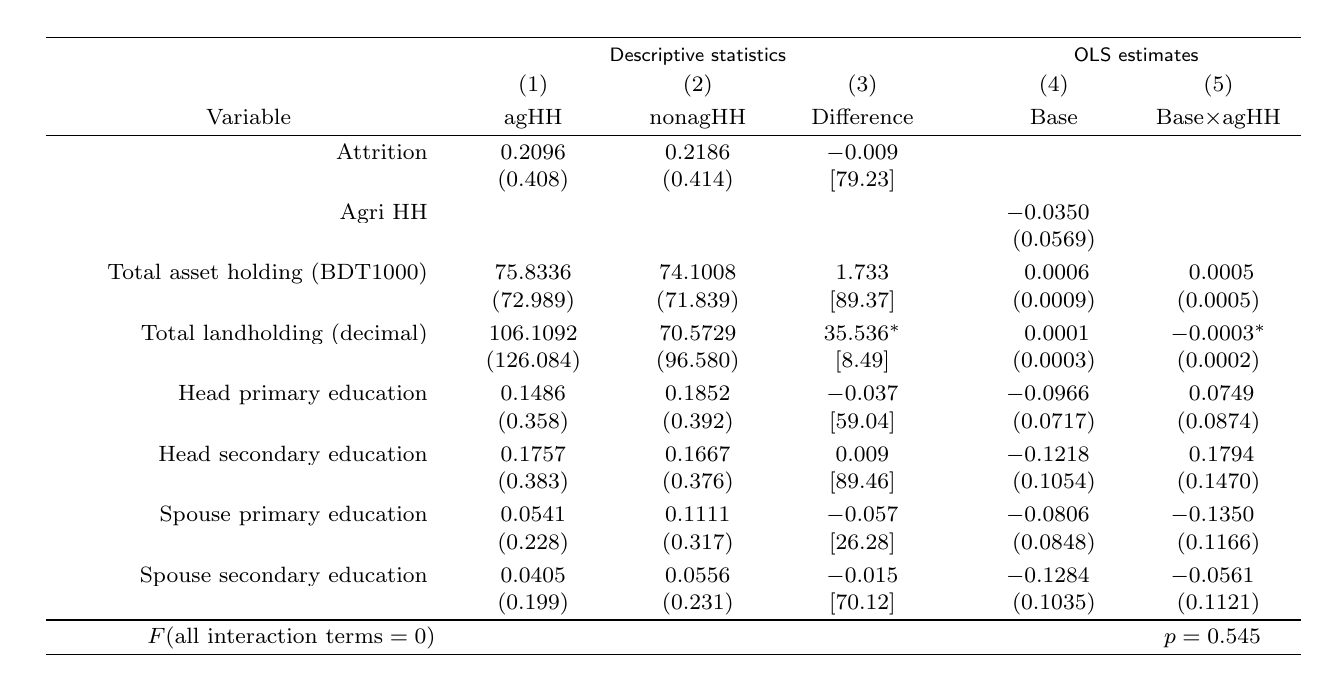
\begin{tikzpicture}
\node (tbl) {
\setlength{\tabcolsep}{2pt}
\begin{tabular}{
>{\footnotesize\hfil$}p{5cm}<{$}
>{\footnotesize\hfil$}p{1.95cm}<{$}
>{\footnotesize\hfil$}p{1.95cm}<{$}
>{\footnotesize\hfil$}p{1.95cm}<{$}
>{$}p{0.2cm}<{$}
>{\footnotesize\hfil$}p{1.95cm}<{$}
>{\footnotesize\hfil$}p{1.95cm}<{$}
>{\footnotesize\hfil$}p{1.95cm}<{$}}
\rowcolor{white}\hline
\makebox[4.75cm]{\scriptsize\hfil}&\multicolumn{3}{c}{\makebox[5.85cm]{\scriptsize \textsf{Descriptive statistics}}}&&\multicolumn{2}{c}{\makebox[3.9cm]{\scriptsize \textsf{OLS estimates}}} \\[-.25ex]
\cline{2-4} \cline{6-7}\rowcolor{white}
 & (1) & (2) & (3) & & (4) & (5)\\
\makebox[4cm]{\cellcolor{white}Variable} & \makebox[1.95cm]{\cellcolor{white}agHH} & \makebox[1.95cm]{\cellcolor{white}nonagHH} & \makebox[1.95cm]{\cellcolor{white}Difference} & \makebox[0.2cm]{\cellcolor{white}} & \makebox[1.95cm]{\cellcolor{white}Base} & \makebox[1.95cm]{\cellcolor{white}Base$\times$agHH}\\
\hline
\makebox[4.75cm]{\hfill Attrition } & 0.2096 & 0.2186 & -0.009 &  &  & \\[-.5ex]
\makebox[4.75cm]{\hfill  } & (0.408) & (0.414) & [79.23] &  &  & \\\rowcolor{white}
\makebox[4.75cm]{\hfill Agri HH } &  &  &  &  & -0.0350\phantom{^{*}} & \\[-.5ex]\rowcolor{white}
\makebox[4.75cm]{\hfill  } &  &  &  &  & (0.0569) & \\
\makebox[4.75cm]{\hfill Total asset holding (BDT1000) } & 75.8336 & 74.1008 & 1.733 &  & \phantom{-}0.0006\phantom{^{*}} & \phantom{-}0.0005\phantom{^{*}}\\[-.5ex]
\makebox[4.75cm]{\hfill  } & (72.989) & (71.839) & [89.37] &  & (0.0009) & (0.0005)\\\rowcolor{white}
\makebox[4.75cm]{\hfill Total landholding (decimal) } & 106.1092 & 70.5729 & 35.536^{*} &  & \phantom{-}0.0001\phantom{^{*}} & -0.0003^{*}\\[-.5ex]\rowcolor{white}
\makebox[4.75cm]{\hfill  } & (126.084) & (96.580) & [8.49] &  & (0.0003) & (0.0002)\\
\makebox[4.75cm]{\hfill Head primary education } & 0.1486 & 0.1852 & -0.037 &  & -0.0966\phantom{^{*}} & \phantom{-}0.0749\phantom{^{*}}\\[-.5ex]
\makebox[4.75cm]{\hfill  } & (0.358) & (0.392) & [59.04] &  & (0.0717) & (0.0874)\\\rowcolor{white}
\makebox[4.75cm]{\hfill Head secondary education } & 0.1757 & 0.1667 & 0.009 &  & -0.1218\phantom{^{*}} & \phantom{-}0.1794\phantom{^{*}}\\[-.5ex]\rowcolor{white}
\makebox[4.75cm]{\hfill  } & (0.383) & (0.376) & [89.46] &  & (0.1054) & (0.1470)\\
\makebox[4.75cm]{\hfill Spouse primary education } & 0.0541 & 0.1111 & -0.057 &  & -0.0806\phantom{^{*}} & -0.1350\phantom{^{*}}\\[-.5ex]
\makebox[4.75cm]{\hfill  } & (0.228) & (0.317) & [26.28] &  & (0.0848) & (0.1166)\\\rowcolor{white}
\makebox[4.75cm]{\hfill Spouse secondary education } & 0.0405 & 0.0556 & -0.015 &  & -0.1284\phantom{^{*}} & -0.0561\phantom{^{*}}\\[-.5ex]\rowcolor{white}
\makebox[4.75cm]{\hfill  } & (0.199) & (0.231) & [70.12] &  & (0.1035) & (0.1121)\\
\hline
\makebox[4.75cm]{\hfill $F (\mbox{all interaction terms}=0)$} &  &  & &  &  & p=0.545\phantom{^{*}}\\\hline
\end{tabular}
};
\end{tikzpicture}\\
\renewcommand{\arraystretch}{.8}
\setlength{\tabcolsep}{1pt}
\hfil\begin{tabular}{>{\hfill\scriptsize}p{1cm}<{}>{\hfill\scriptsize}p{.25cm}<{}>{\scriptsize}p{13.75cm}<{\hfill}}
Source:& \multicolumn{2}{l}{\scriptsize Compiled from IFPRI data.}\\
Notes: & 1. & Attrition is true if a household is missing in round 2. All covariates are of round 1.\\
& 2. & \textsf{Descriptive statistics} panel shows attriter's characteristics. The top rows show the means, and the bottom rows show the standard errors in columns (1) and (2), respectively. In column (3), the top rows show mean differences, and the bottom rows show associated $p$ values of mean differences in percentage. \textsf{OLS estimation} panel shows results from a linear probability model of attrition on baseline variables $\bfx_{i}$ and their interaction with the agricultural household dummy $r_{i}$: $y_{i}=\bfbeta'\bfx_{i}+\bfgamma'r_{i}\bfx_{i}+e_{i}$. The top rows show point estimates, and the bottom rows show standard errors. Estimates of non-agricultural HHs $\bfbeta$ are shown in (4), and interaction terms $\bfgamma$ of each variable with agricultural HH are shown in (5). Number of observations for LPM is $570$, $\bar{R}=0.058$. Standard errors are shown in parentheses, which are clustered at the Thana level with a Satterthwaite correction for a small number of clusters. For column (3), $p$ values of the null of zero difference are shown in square brackets. $*$ indicates a $p$ value between 5\% and 10\%. 
\end{tabular}
\end{minipage}
\end{table}

%We also tested for nonrandom attrition and found that only agricultural households' land holding is weakly correlated, and we use it as a control in all estimations. See of this appendix. In our main regression specification, we control for the child's age. In addition, our main findings of this study \sout{remain largely consistent} \SAdded{comes mainly from boys around 11-17 yeas old (secondary school ages), so the results remain unchanged} when we use the 735 samples \SAdded{as it retains these cohorts}. \sout{and these estimates are available upon request.}

%\begin{table}[bp]
%\caption{Original vs. regression data contrasts: main sample}
%\label{origregcontrast}
%\begin{center}
%{
%\resizebox{14.5cm}{!}{
%\begin{tabular}{lccccc}
%\hline
%Variables                                       & Original & Regression & T-stat & $\chi^{2}$ & Binomial \\
%                                                & Sample & Sample  &  & & \\
%\hline
%Agricultural household                          & 0.6027 & 0.5968 & 0.8196 & 0.8618 & 0.7544\\
%Agricultural household (head)                   & 0.5619 & 0.5587 & 0.9020 & 0.9444 & 0.8774\\
%Child's Age                                     & 13.4313 & 13.0132 & 0.0025 &    NA &    NA\\
%Child's Sex (female = 1)                        & 0.5007 & 0.5103 & 0.7187 & 0.7586 & 0.6189\\
%Head education: primary                         & 0.3537 & 0.3592 & 0.8293 & 0.8726 & 0.7793\\
%Head secondary: secondary                       & 0.2381 & 0.2346 & 0.8773 & 0.9267 & 0.8574\\
%Spouse's sex (female = 1)                       & 0.9293 & 0.9296 & 0.9785 & 1.0000 & 1.0000\\
%Spouse education: primary                       & 0.3156 & 0.3167 & 0.9655 & 1.0000 & 0.9671\\
%Spouse education: secondary                     & 0.2544 & 0.2610 & 0.7776 & 0.8243 & 0.6924\\
%Per member land holding (Acre, in 1999)         & 0.1814 & 0.1751 & 0.6886 &  NA &  NA\\
%Per member non-land asset (1000 BDT, in 1999)   & 11.5303 & 11.4060 & 0.8710 & NA & NA\\
%Paddy yield (annual, thana level)               & 0.7834 & 0.7841 & 0.9066 &    NA &    NA\\
%Household has structured toilet (dummy)         & 0.2925 & 0.2933 & 0.9757 & 1.0000 & 0.9664\\
%Household has access to piped water (dummy)     & 0.3687 & 0.3724 & 0.8847 & 0.9282 & 0.8428\\
%Observations                                    & 735 & 682 &  &  & \\
%\hline
%\multicolumn{6}{p{18cm}}{{\footnotesize Notes: All information is based on first round of data set, which was collected in 1999. Column headed by $T-Stat$ shows $p$ values of equal means for both data sets using $t$ tests. Column headed by $\chi^{2}$ shows $p$ values of equal proportions. Column headed by \textsf{Binomial} shows $p$ values of two-sided test for one proportion being equal to another proportion under presumed Bernoulli trials. Agricultural household are defined as at least one adult member claiming that main income source as agriculture, agricultural household (head) is defined as head is claiming that main income source is agriculture. Age and sex are of children of the households.}}
%\end{tabular}}}
%\end{center}
%\end{table}

Table \ref{tab destat zEm1999} summarizes the data used in the regressions. Based on the age cut-off of 10 years and older in the 1999 survey, we have 626 observations. In our sample, approximately 61 percent of households were categorized as agricultural households. Alternative agricultural household definitions give similar summary statistics, which explains the small difference in estimation. The household head's highest level of education is mostly secondary, 28\%, and the primary level comprises 15.5\% of our sample. Spousal education is similar for the primary level, 17\%, but relatively low for the secondary level, 16.6\%. The mean per member landholding is 0.168 acre. Median per member non-land assets are about 11,000 BDT (110 USD), and about 14,000 BDT (140 USD) at the 75th percentile. These non-land asset values indicate that our sample primarily comprises poor rural households.

For the placebo sample, we took 10 to 18 years in 2002 (2002 cohort) to compare with the main data. \textsc{Table \ref{tab destat zEp2002}} presents a summary of the data used in the placebo regressions. Based on the age cutoff of 10 years and older in the 2002 survey, there are 812 observations in the placebo sample. In our placebo sample, we have about 60\% agricultural households, which is quite similar to the main sample. Other summary statistics reported in Table \ref{tab destat zEm1999} show close similarity with Table \ref{tab destat zEp2002}. This demonstrates the validity of a placebo sample, at least observational. The only notable observable difference between these two samples, however, is the declining enrollment rate, which is about 11 percentage points lower than the 1999 average.

\begin{minipage}[t]{.8\paperwidth}
\hfil\textsc{\normalsize Table \refstepcounter{table}\thetable: \begin{minipage}[t]{.6\paperwidth}
Descriptive statistics of main estimation,\\ 10-18 years old, direct offspring\setlength{\baselineskip}{8pt}
\end{minipage}
\label{tab destat zEm1999}}\\
\setlength{\tabcolsep}{1pt}
\renewcommand{\arraystretch}{.6}
\hfil\begin{tabular}{>{\scriptsize}p{5cm}<{\hfill}>{\hfill\scriptsize$}p{0.75cm}<{$}>{\hfill\scriptsize$}p{0.75cm}<{$}>{\hfill\scriptsize$}p{0.75cm}<{$}>{\hfill\scriptsize$}p{0.75cm}<{$}>{\hfill\scriptsize$}p{0.75cm}<{$}>{\hfill\scriptsize$}p{1cm}<{$}>{\hfill\scriptsize$}p{0.75cm}<{$}>{\hfill\scriptsize$}p{0.75cm}<{$}>{\hfill\scriptsize$}p{0.75cm}<{$}>{\hfill\scriptsize$}p{0.75cm}<{$}}
\makebox[5cm]{covariates} & \makebox[0.75cm]{min} & \makebox[0.75cm]{25\%} & \makebox[0.75cm]{median} & \makebox[0.75cm]{75\%} & \makebox[0.75cm]{max} & \makebox[1cm]{mean} & \makebox[0.75cm]{std} & \makebox[0.75cm]{0s} & \makebox[0.75cm]{NAs} & \makebox[0.75cm]{n}\\
Enrolled & 0 & 0 & 1 & 1 & 1 & 0.738 & 0.440 & 164 & 0 & 626\\
Agricultural household (combined) & 0 & 0 & 1 & 1 & 1 & 0.613 & 0.487 & 242 & 0 & 626\\
Agricultural household (head definition) & 0 & 0 & 1 & 1 & 1 & 0.553 & 0.498 & 280 & 0 & 626\\
Agricultural household (income definition) & 0 & 0 & 1 & 1 & 1 & 0.575 & 0.495 & 266 & 0 & 626\\
Agricultural household (occupation definition) & 0 & 0 & 1 & 1 & 1 & 0.543 & 0.499 & 286 & 0 & 626\\
Membership to stipend program & 0 & 0 & 0 & 1 & 1 & 0.315 & 0.465 & 429 & 0 & 626\\
Membership to non-stipend program & 0 & 0 & 0 & 1 & 1 & 0.425 & 0.495 & 360 & 0 & 626\\
Sex & 0 & 0 & 1 & 1 & 1 & 0.511 & 0.500 & 306 & 0 & 626\\
Head sex (female = 1) & 0 & 0 & 0 & 0 & 1 & 0.128 & 0.334 & 546 & 0 & 626\\
Non-Muslim & 0 & 0 & 0 & 0 & 1 & 0.123 & 0.329 & 549 & 0 & 626\\
Flooded & 0 & 0 & 1 & 1 & 1 & 0.623 & 0.485 & 236 & 0 & 626\\
Structured toilet & 0 & 0 & 0 & 1 & 1 & 0.294 & 0.456 & 442 & 0 & 626\\
\hspace{.5em}Own piped water & 0 & 0 & 0 & 1 & 1 & 0.380 & 0.486 & 388 & 0 & 626\\
head primary & 0 & 0 & 0 & 0 & 1 & 0.155 & 0.362 & 529 & 0 & 626\\
head secondary & 0 & 0 & 0 & 1 & 1 & 0.284 & 0.451 & 448 & 0 & 626\\
head spouse primary & 0 & 0 & 0 & 0 & 1 & 0.171 & 0.377 & 519 & 0 & 626\\
head spouse secondary & 0 & 0 & 0 & 0 & 1 & 0.166 & 0.372 & 522 & 0 & 626\\
age & 10 & 11 & 13 & 15 & 18 & 12.986 & 2.351 & 0 & 0 & 626\\
yield (thana) & 0.607 & 0.647 & 0.823 & 0.906 & 0.928 & 0.786 & 0.110 & 0 & 0 & 626\\
Number of older female siblings & 0 & 0 & 0 & 1 & 4 & 0.390 & 0.670 & 434 & 0 & 626\\
Number of older male siblings & 0 & 0 & 0 & 1 & 5 & 0.577 & 0.844 & 376 & 0 & 626\\
per member land holding (decimal, in 1999) & 0 & 0.019 & 0.069 & 0.196 & 3.215 & 0.167 & 0.287 & 2 & 0 & 626\\
per member nonland asset (1000 Tk, in 1999) & 0.373 & 3.918 & 7.062 & 13.623 & 205 & 11.209 & 14.515 & 0 & 0 & 626\\
\end{tabular}
\\

\renewcommand{\arraystretch}{.55}
\setlength{\tabcolsep}{1pt}
\begin{tabular}{>{\hfill\scriptsize}p{1cm}<{}>{\hfill\scriptsize}p{.25cm}<{}>{\scriptsize}p{.6\paperwidth}<{\hfill}}
Source:& \multicolumn{2}{l}{\scriptsize Compiled from IFPRI data.}\\
Notes: & 1. & All information is of year 1999.\\
& 2. & Agricultural households are defined as at least one adult member claiming that the main income source is agriculture or occupation is agriculture. Program membership is one if holding a membership to anti-poverty programs. STD represents Standard deviation.\setlength{\baselineskip}{6pt}
\end{tabular}
\end{minipage}



%\begin{table}[t]
%\caption{Descriptive Statistics: Main sample}
%\label{tab_destat}
%\begin{center}
%{
%\resizebox{14.5cm}{!}{
%\begin{tabular}{lcccccccccc}
%\hline
%Variables                           & Min & 25\% & Median & 75\% & Max & Mean & STD & `0's & `NA's & n\\
%\hline
%Enrolled & 0 & 0 & 1 & 1 & 1 & 0.73 & 0.44 & 184 & 0 & 682\\
%Agricultural household & 0 & 0 & 1 & 1 & 1 & 0.6 & 0.49 & 275 & 0 & 682\\
%Agricultural household (head) & 0 & 0 & 1 & 1 & 1 & 0.56 & 0.5 & 301 & 0 & 682\\
%Program membership & 0 & 0 & 1 & 1 & 1 & 0.73 & 0.44 & 183 & 0 & 682\\
%Child's Age & 10 & 11 & 13 & 15 & 18 & 13.01 & 2.38 & 0 & 0 & 682  \\
%Child's Sex (female = 1) & 0 & 0 & 1 & 1 & 1 & 0.51 & 0.5 & 334 & 0 & 682\\
%Head education: primary  & 0 & 0 & 0 & 1 & 1 & 0.36 & 0.48 & 437 & 0 & 682\\
%Head secondary: secondary & 0 & 0 & 0 & 0 & 1 & 0.23 & 0.42 & 522 & 0 & 682\\
%Spouse education: primary & 0 & 0 & 0 & 1 & 1 & 0.32 & 0.47 & 466 & 0 & 682\\
%Spouse education: secondary & 0 & 0 & 0 & 1 & 1 & 0.26 & 0.44 & 504 & 0 & 682\\
%Per member land holding (acre, in 1999) & 0 & 0.018 & 0.066 & 0.19 & 3.215 & 0.168 & 0.294 & 2 & 0 & 682\\
%Per member non-land asset (1000 BDT, in 1999) & 0.369 & 3.537 & 6.963 & 13.557 & 205 & 11.017 & 14.649 & 0 & 0 & 682\\
%Paddy yield (annual, thana level) & 0.61 & 0.65 & 0.82 & 0.91 & 0.93 & 0.78 & 0.11 & 0 & 0 & 682\\
%Household has Structured toilet (dummy) & 0 & 0 & 0 & 1 & 1 & 0.29 & 0.46 & 482 & 0 & 682\\
%Household has access to piped water (dummy) & 0 & 0 & 0 & 1 & 1 & 0.37 & 0.48 & 428 & 0 & 682\\
%Mean low temperature (annual, thana level) & 20.77 & 21.24 & 21.32 & 22.35 & 22.59 & 21.6 & 0.63 & 0 & 0 & 682\\
%Mean high temperature (annual, thana level) & 30.11 & 30.69 & 31.18 & 31.61 & 32.33 & 31.15 & 0.66 & 0 & 0 & 682\\
%Mean clear sky indicator (annual, thana level) & 0.15 & 0.2 & 0.22 & 0.23 & 0.3 & 0.22 & 0.05 & 0 & 0 & 450\\
%Mean cloud coverage (0-1, annual, thana level) & 0.46 & 0.47 & 0.51 & 0.52 & 0.53 & 0.5 & 0.03 & 0 & 0 & 450\\
%Mean temperature (annual, thana level) & 76.08 & 77.57 & 77.94 & 78.42 & 79.56 & 77.91 & 0.97 & 0 & 0 & 682\\
%STD clear sky indicator (annual, thana level) & 0.35 & 0.4 & 0.42 & 0.42 & 0.46 & 0.41 & 0.03 & 0 & 0 & 450\\
%STD cloud coverage (0-1, annual, thana level) & 0.32 & 0.32 & 0.35 & 0.36 & 0.4 & 0.35 & 0.02 & 0 & 0 & 450\\
%STD temperature (annual, thana level) & 6.24 & 8.02 & 8.83 & 9.12 & 9.64 & 8.47 & 1.09 & 0 & 0 & 450\\
%\hline
%\multicolumn{11}{p{22cm}}{{\footnotesize Notes: All information is based on first round of data set, which was collected in 1999. Agricultural household is an indicator variable for a household whose primary income is agriculture. Agricultural household (head) is defined as head is claiming that main income source is agriculture. Program membership is 1 if at least one household membership receive either safety net or education related program (stipend/scholarship) support. Age and sex are of children of the households. STD represents Standard deviation.}}
%\end{tabular}}}
%\end{center}
%\end{table}

\begin{minipage}[t]{.8\paperwidth}
\hfil\textsc{\normalsize Table \refstepcounter{table}\thetable: \begin{minipage}[t]{.6\paperwidth}
Descriptive statistics of placebo estimation,\\ 10-18 years old in 2002, direct offspring
\setlength{\baselineskip}{8pt}
\end{minipage}
\label{tab destat zEp2002}}\\
\setlength{\tabcolsep}{1pt}
\renewcommand{\arraystretch}{.6}
\hfil\begin{tabular}{>{\scriptsize\hfill}p{5.75cm}<{}>{\hfill\scriptsize$}p{0.85cm}<{$}>{\hfill\scriptsize$}p{0.85cm}<{$}>{\hfill\scriptsize$}p{0.85cm}<{$}>{\hfill\scriptsize$}p{0.85cm}<{$}>{\hfill\scriptsize$}p{0.85cm}<{$}>{\hfill\scriptsize$}p{1cm}<{$}>{\hfill\scriptsize$}p{0.85cm}<{$}>{\hfill\scriptsize$}p{0.85cm}<{$}>{\hfill\scriptsize$}p{0.85cm}<{$}>{\hfill\scriptsize$}p{0.85cm}<{$}}
\makebox[5.75cm]{covariates} & \makebox[0.85cm]{min} & \makebox[0.85cm]{25\%} & \makebox[0.85cm]{median} & \makebox[0.85cm]{75\%} & \makebox[0.85cm]{max} & \makebox[1cm]{mean} & \makebox[0.85cm]{std} & \makebox[0.85cm]{0s} & \makebox[0.85cm]{NAs} & \makebox[0.85cm]{n}\\
\hline
Enrolled & 0 & 0 & 1 & 1 & 1 & 0.631 & 0.483 & 300 & 0 & 812\\
Agricultural household (combined definition) & 0 & 0 & 1 & 1 & 1 & 0.606 & 0.489 & 320 & 0 & 812\\
Agricultural household (head definition) & 0 & 0 & 1 & 1 & 1 & 0.542 & 0.499 & 372 & 0 & 812\\
Agricultural household (income definition) & 0 & 0 & 1 & 1 & 1 & 0.562 & 0.496 & 356 & 0 & 812\\
Agricultural household (occupation definition) & 0 & 0 & 1 & 1 & 1 & 0.537 & 0.499 & 376 & 0 & 812\\
Membership to stipend program & 0 & 0 & 0 & 1 & 1 & 0.273 & 0.446 & 590 & 0 & 812\\
Membership to non-stipend program & 0 & 0 & 0 & 0 & 1 & 0.002 & 0.050 & 810 & 0 & 812\\
Sex (female = 1) & 0 & 0 & 1 & 1 & 1 & 0.525 & 0.500 & 386 & 0 & 812\\
Head sex (female = 1) & 0 & 0 & 0 & 0 & 1 & 0.116 & 0.320 & 718 & 0 & 812\\
Flooded & 0 & 0 & 1 & 1 & 1 & 0.626 & 0.484 & 304 & 0 & 812\\
Structured toilet & 0 & 0 & 0 & 1 & 1 & 0.282 & 0.450 & 583 & 0 & 812\\
\hspace{.5em}Own piped water & 0 & 0 & 0 & 1 & 1 & 0.376 & 0.485 & 507 & 0 & 812\\
Head education: primary & 0 & 0 & 0 & 0 & 1 & 0.159 & 0.366 & 683 & 0 & 812\\
Head education: secondary & 0 & 0 & 0 & 1 & 1 & 0.281 & 0.450 & 584 & 0 & 812\\
Head's spouse education: primary & 0 & 0 & 0 & 0 & 1 & 0.177 & 0.382 & 668 & 0 & 812\\
Head's spouse education: secondary & 0 & 0 & 0 & 0 & 1 & 0.166 & 0.373 & 677 & 0 & 812\\
Age & 10 & 12 & 13 & 16 & 18 & 13.631 & 2.470 & 0 & 0 & 812\\
Yield (thana) & 0.69 & 0.743 & 0.838 & 0.984 & 1.036 & 0.848 & 0.117 & 0 & 0 & 812\\
Number of older female siblings & 0 & 0 & 0 & 1 & 4 & 0.560 & 0.793 & 477 & 0 & 812\\
Number of older male siblings & 0 & 0 & 0 & 1 & 5 & 0.659 & 0.882 & 447 & 0 & 812\\
Per member land holding (decimal, in 1999) & 0 & 0.017 & 0.063 & 0.179 & 3.215 & 0.160 & 0.289 & 2 & 0 & 812\\
Per member nonland asset (1000 Tk, in 1999) & 0.369 & 3.537 & 6.963 & 13.143 & 205 & 10.994 & 14.995 & 0 & 0 & 812\\
\end{tabular}
\\

\renewcommand{\arraystretch}{.55}
\setlength{\tabcolsep}{1pt}
\begin{tabular}{>{\hfill\scriptsize}p{1cm}<{}>{\hfill\scriptsize}p{.25cm}<{}>{\scriptsize}p{.6\paperwidth}<{\hfill}}
Source:& \multicolumn{2}{l}{\scriptsize Compiled from IFPRI data.}\\
Notes: & 1. & All information is of year 2002 except for \textsf{Enrolled, Yield, Temperature, Rainfall, Program membership}.\\
& 2. & Agricultural households are defined as at least one adult member claiming that the main income source is agriculture or occupation is agriculture. Program membership is one of holding a membership to anti-poverty programs. STD represents Standard deviation. \setlength{\baselineskip}{6pt}
\end{tabular}
\end{minipage}

\pagebreak


%\begin{table}[t]
%\caption{Descriptive Statistics: placebo sample}
%\label{tab_destat2}
%\begin{center}
%{
%\resizebox{14.5cm}{!}{
%\begin{tabular}{lcccccccccc}
%\hline
%Variables                 & Min & 25\% & Median & 75\% & Max & Mean & STD & `0's & `NA's & n\\
%\hline
%Enrolled & 0 & 0 & 1 & 1 & 1 & 0.62 & 0.48 & 327 & 0 & 870\\
%Agricultural household & 0 & 0 & 1 & 1 & 1 & 0.58 & 0.49 & 362 & 0 & 870\\
%Agricultural household (head) & 0 & 0 & 1 & 1 & 1 & 0.55 & 0.5 & 388 & 0 & 870\\
%Program membership & 0 & 0 & 0 & 1 & 1 & 0.26 & 0.44 & 640 & 0 & 870\\
%Child's Age & 10 & 12 & 13 & 16 & 18 & 13.64 & 2.47 & 0 & 0 & 870\\
%Child's Sex (female = 1) & 0 & 0 & 1 & 1 & 1 & 0.53 & 0.5 & 413 & 0 & 870\\
%Head education: primary  & 0 & 0 & 0 & 1 & 1 & 0.34 & 0.48 & 570 & 0 & 870\\
%Head secondary: secondary & 0 & 0 & 0 & 0.75 & 1 & 0.25 & 0.43 & 652 & 0 & 870\\
%Spouse education: primary & 0 & 0 & 0 & 1 & 1 & 0.27 & 0.45 & 632 & 0 & 870\\
%Spouse education: secondary & 0 & 0 & 0 & 1 & 1 & 0.27 & 0.45 & 632 & 0 & 870\\
%Per member land holding (acre, in 1999) & 0 & 0.018 & 0.066 & 0.19 & 3.215 & 0.168 & 0.294 & 2 & 0 & 682\\
%Per member non-land asset (1000 BDT, in 1999) & 0.369 & 3.537 & 6.963 & 13.557 & 205 & 11.017 & 14.649 & 0 & 0 & 682\\
%Paddy yield (annual, thana level) & 0.69 & 0.74 & 0.84 & 0.98 & 1.04 & 0.85 & 0.12 & 0 & 0 & 870\\
%Household has Structured toilet (dummy) & 0 & 0 & 0 & 1 & 1 & 0.28 & 0.45 & 624 & 0 & 870\\
%Household has access to piped water (dummy) & 0 & 0 & 0 & 1 & 1 & 0.37 & 0.48 & 546 & 0 & 870\\
%Mean low temperature (annual, thana level) & 20.5 & 20.77 & 20.98 & 21.79 & 22.52 & 21.23 & 0.67 & 0 & 0 & 870\\
%Mean high temperature (annual, thana level) & 29.31 & 29.47 & 30.41 & 30.75 & 31.95 & 30.38 & 0.81 & 0 & 0 & 870\\
%\hline
%\multicolumn{11}{p{22cm}}{{\footnotesize Notes: All information is based on second round of data set, which was collected in 2002. Agricultural household are defined as at least one adult member claiming that main income source as agriculture, agricultural household (head) is defined as head is claiming that main income source is agriculture. Program membership is 1 if at least one household membership receive either safety net or education related program (stipend/scholarship) support. Age and sex are of children of the households. STD represents Standard deviation.}}
%\end{tabular}}}
%\end{center}
%\end{table}


%{\color{red}
%\begin{minipage}[t]{.8\paperwidth}
%\hfil\textsc{\normalsize Table \refstepcounter{table}\thetable: \begin{minipage}[t]{.5\paperwidth}
%Descriptive statistics\\ by different definitions of  agricultural HHs\setlength{\baselineskip}{8pt}
%\end{minipage}\label{destat ag diff defs}}\\

%\setlength{\tabcolsep}{1pt}
%\renewcommand{\arraystretch}{.575}
%\hfil\input{Tables/AgDefComparisonCRSE_JHR.tex}\\

%\renewcommand{\arraystretch}{.7}
%\hfil\begin{tabular}{>{\hfill\scriptsize}p{1cm}<{}>{\scriptsize}p{12cm}<{\hfill}}
%Source:& Compiled from IFPRI data. All information is of year 1999.\\
%Notes: & For each variable, top rows show means. Bottom rows show 95\% confidence intervals. Standard errors are clustered at thana level and Satterthwaite correction for degree of freedom is applied to account for small number of clusters. \textsf{isagHH} is at least one adult member claiming that main income source as agriculture. \textsf{hdagHH} is household head reports that main income source as agriculture. \textsf{occagHH} is at least one adult member claiming that occupation as agriculture. \textsf{agHH0} is a union of \textsf{isagHH}, \textsf{hdagHH}, and \textsf{occagHH}.\setlength{\baselineskip}{8pt} 
%\end{tabular}

%\end{minipage}

%\vspace{2ex}
%%\textsc{\normalsize Table \ref{destat ag diff defs}} shows descriptive statistics by alternative agricultural household definitions. \textsf{isagHH} is at least one adult member claiming that main income source as agriculture. \textsf{hdagHH} is household head reports that main income source as agriculture. \textsf{ocagHH} is at least one adult member claiming that occupation as agriculture. Our default definition \textsf{agHH0} is a union of \textsf{isagHH}, \textsf{hdagHH}, and \textsf{ocagHH}. We see that they are all similar. We note that the choice of particular definition does not change the results qualitatively. We also note that 9.7\% of \textsf{ocagHH} is associated with non-agricultural work as the main income source, and is likely to be more measurement error prone and attenuated. Consistent with this, the impact estimates are closer to zero when we use the \textsf{ocagHH} definition.\footnote{\SAdded{This implies that the main estimates using our default definition are also attenuated. This can be seen in a comparison with head based definition in \textsc{Table \ref{base10}}. However, we will use the most inclusive definition of agricultural household as our default definition and show results using other definitions as a part of robustness checks.} }
 % end of red ink



%\textsc{Table \ref{MainByGenderByAgeLBAgHH0Results}} shows gender wise results with various age lowerbounds. It shows higher age lowerbounds are associated with lager impact estimates on boys.

%\textsc{Table \ref{PlaceboResults10Table}} shows placebo test results at disaggregated by gender. Both 1999 cohort and 2002 cohort give estimates that are statistically zero.

To assess relative impoverishment, we tabulated agriculture and non-agricultural households based on household consumption information in Table \ref{agpc4}. The consumption quartiles are derived based on per-member consumption information in the household. We noticed a higher consumption quartile for non-agricultural households compared to Agricultural households.

The IFPRI panel data set reports reasons for dropping out of school (\textsc{\small Table \ref{reasons}}). We notice dropout rates are higher for lower consumption quartiles, and their reasons for dropping out primarily include financial difficulties, which is also true for irregular students. Upper-quartile individuals cite non-financial reasons such as marriage as the reason for drop-out. We also summarize the reported reasons for school dropout by household type in {\textsc{\small Table \ref{reasons2}}: agricultural or non-agricultural households. Our table indicates that agricultural households cite financial reasons more frequently than non-agricultural ones as the main reason for dropping out and school irregularity. 

\begin{table}
\caption{Tabulation of Agricultural vs. Non-Agriculture household Consumption Quartiles}
\label{agpc4}
\begin{center}
{
\resizebox{11.5cm}{!}{
\begin{tabular}{lcccccc}
\hline
Quartiles & 1     & 2         & 3          & 4        & `NA's         &       N    \\
\hline
Agricultural households  & 25.8 &      27.27 &      26.54 &      19.66 & 0.74 &   407 \\
Non-agricultural households & 23.27 &  24.36 &  18.55 &   33.82 &   0 &        275 \\
\hline
\hline
\multicolumn{7}{p{12cm}}{{\footnotesize Notes: Consumption quartiles are based on households.}}
\end{tabular}}}
\end{center}
\end{table}

\begin{table}[bp]
\caption{Reported Reasons for Stop Going to School by Consumption Quartiles and by Household Type}
\label{reasons}
\begin{center}
{
\resizebox{15cm}{!}{
\begin{tabular}{cccccccccc}
\hline
Quartile & Group & \scriptsize{Financial} & \scriptsize {Not accepted} & \scriptsize {School environment} & \scriptsize {Marriage} & \scriptsize {Distance} & \scriptsize {Sickness} & NA & Total                        \\
\hline
1 & Irregular 1999 &  0.52 &  0.03 &  0.2 & 0    & 0.06 & 0.02 & 0.17 & 65 \\
1 & Irregular 2002 &  0.54 &  0.01 & 0.01 & 0.01 & 0.01 &    0 & 0.43 & 115 \\
1 & Drop outs 2002 &  0.62 &     0 & 0.02 & 0.02 &    0 &    0 & 0.34 &  58 \\
\hline
2 & Irregular 1999 &  0.48 &    0 &    0.23 &     0 &   0.14 &    0  &    0.14 &   56 \\
2 & Irregular 2002 &  0.37 &    0 &    0.06 &  0.01 &   0.02 &  0.01 &    0.52 &   81 \\
2 & Drop outs 2002 &  0.41 &    0 &    0.08 &     0 &   0.03 &     0 &    0.49 &   37 \\
\hline
3 & Irregular 1999 &   0.44 &      0 &    0.26 &     0 &     0.18 &    0.09 &    0.03 &   34 \\
3 & Irregular 2002 &   0.28 &      0 &       0 &  0.05 &     0.03 &    0.03 &    0.61 &   64 \\
3 & Drop outs 2002 &   0.26 &      0 &       0 &  0.05 &     0.03 &    0.03 &    0.63 &   38 \\
\hline
4 & Irregular 1999 &   0.45 &   0.05 &   0.18 &      0 &    0.05 &    0.05 &    0.23 &    22 \\
4 & Irregular 2002 &    0.1 &   0.01 &   0.03 &   0.03 &    0.01 &    0.03 &    0.79 &    73 \\
4 & Drop outs 2002 &   0.11 &   0.02 &   0.02 &   0.04 &       0 &    0.04 &    0.78 &    54 \\
\hline\\
\hline
\multicolumn{10}{p{21cm}}{{\footnotesize Notes: Numbers are all ratios except totals. ``Agri HH'' indicates agricultural households. See main text for definition of agricultural households. Irregulars are individuals who were not enrolled in the respective period. Dropouts are individuals who were enrolled in 1999 but not in 2002..}}
\end{tabular}}}
\end{center}
\end{table}



\begin{table}[bp]
\caption{Reasons for Not Going to School, Agricultural vs. Non-Agriculture household}
\label{reasons2}
\begin{center}
{
\resizebox{14.5cm}{!}{
\begin{tabular}{cccccccccc}
\hline
{\bf HH Type} & {\bf Group} & {\bf Financial} & {\bf Not accepted} & {\bf School Environment} & {\bf Marriage} & {\bf Distance} & {\bf Sickness} &   {\bf NA} & {\bf Total} \\
\hline
Ag      & Irregular 1999 &  0.55 &  0.03 &  0.21 &    0 &  0.06 &   0.05 &   0.11 &   66 \\
Ag      & Irregular 2002 &  0.38 &     0 &  0.01 & 0.01 &  0.01 &   0.02 &   0.57 &  120 \\
Ag      & drop outs 2002 &  0.46 &     0 &  0.01 &    0 &  0.01 &   0.01 &    0.5 &   70 \\
\hline
Non-ag  & Irregular 1999 &  0.46 &  0.01 &  0.22 &    0 &  0.13 &   0.02 &   0.16 &  112 \\
Non-ag  & Irregular 2002 &  0.33 &  0.01 &  0.03 & 0.03 &  0.02 &   0.01 &   0.56 &  214 \\
Non-ag  & drop outs 2002 &   0.3 &  0.01 &  0.03 & 0.04 &  0.01 &   0.02 &   0.59 &  117 \\
\hline
\hline
\multicolumn{10}{p{22cm}}{{\footnotesize Notes: Numbers are all ratios except totals. ``Agri HH'' indicates agricultural households. See the main text for the definition of agricultural households. Irregulars are individuals who were not enrolled in the respective period. Dropouts are individuals who were enrolled in 1999 but not in 2002..}}
\end{tabular}}}
\end{center}
\end{table}



\begin{figure}[h!]
%\hspace{-2em}\begin{minipage}[t]{13cm}
\hfil\textsc{\footnotesize Figure \refstepcounter{figure}\thefigure: Enrollment rates by age and HH type, 1999, 5 years and older\label{ERbyAge rawdata}}\\
\hfil 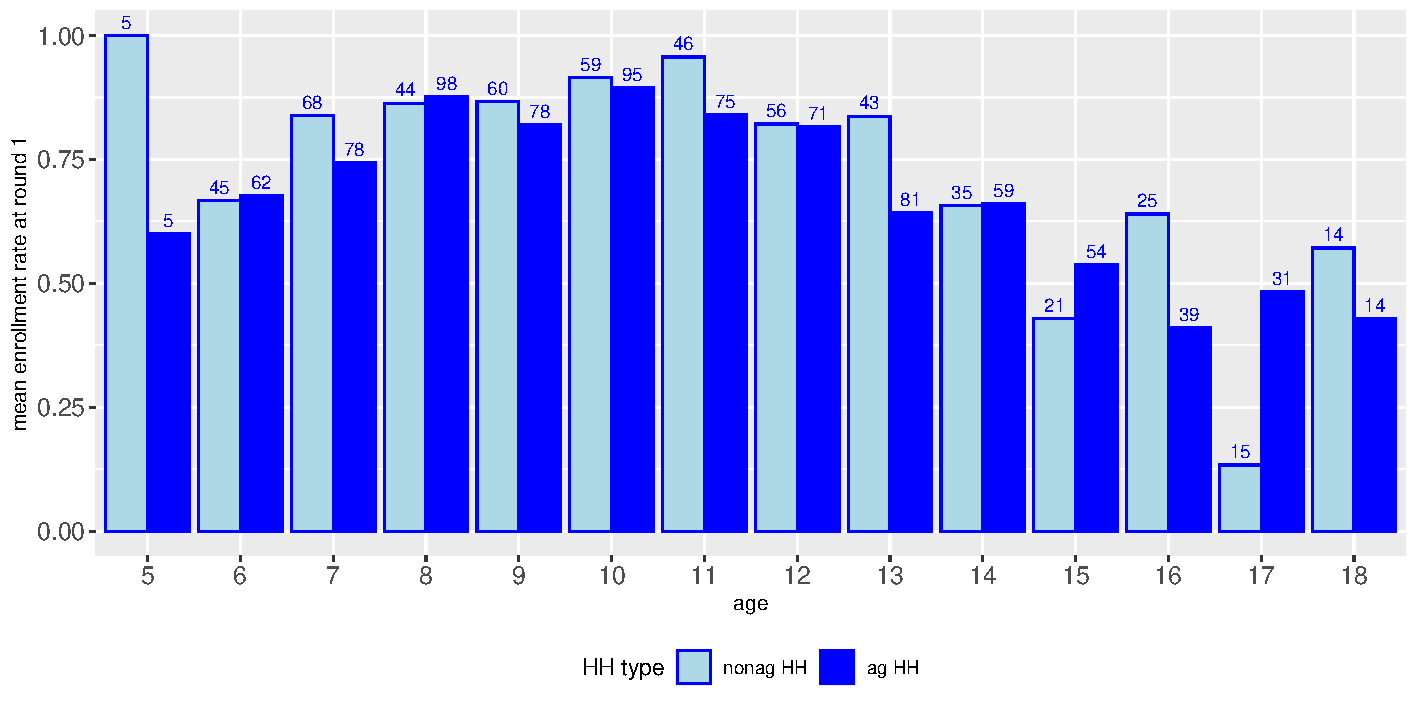
\includegraphics[width=.7\paperwidth]{AgewiseRawEnrollmentRates.pdf}\\
\renewcommand{\arraystretch}{1}
\hfil\begin{tabular}{>{\hfill\scriptsize}p{1cm}<{}>{\scriptsize}p{12cm}<{\hfill}}
Source:& Compiled from IFPRI data. All households, including attrited households, are used.\\[-1ex]
Notes:& Ages are of round 1. Numbers displayed above the bar are cell sample size. \\[-1ex]
\end{tabular}
%\end{minipage}
\end{figure}

\begin{figure}[h!]
%\hspace{-2em}\begin{minipage}[t]{13cm}
\hfil\textsc{\footnotesize Figure \refstepcounter{figure}\thefigure: Age starting the primary school by year and HH type, reported in 2000\label{AgeAtClass1byAge rawdata}}\\
\hfil 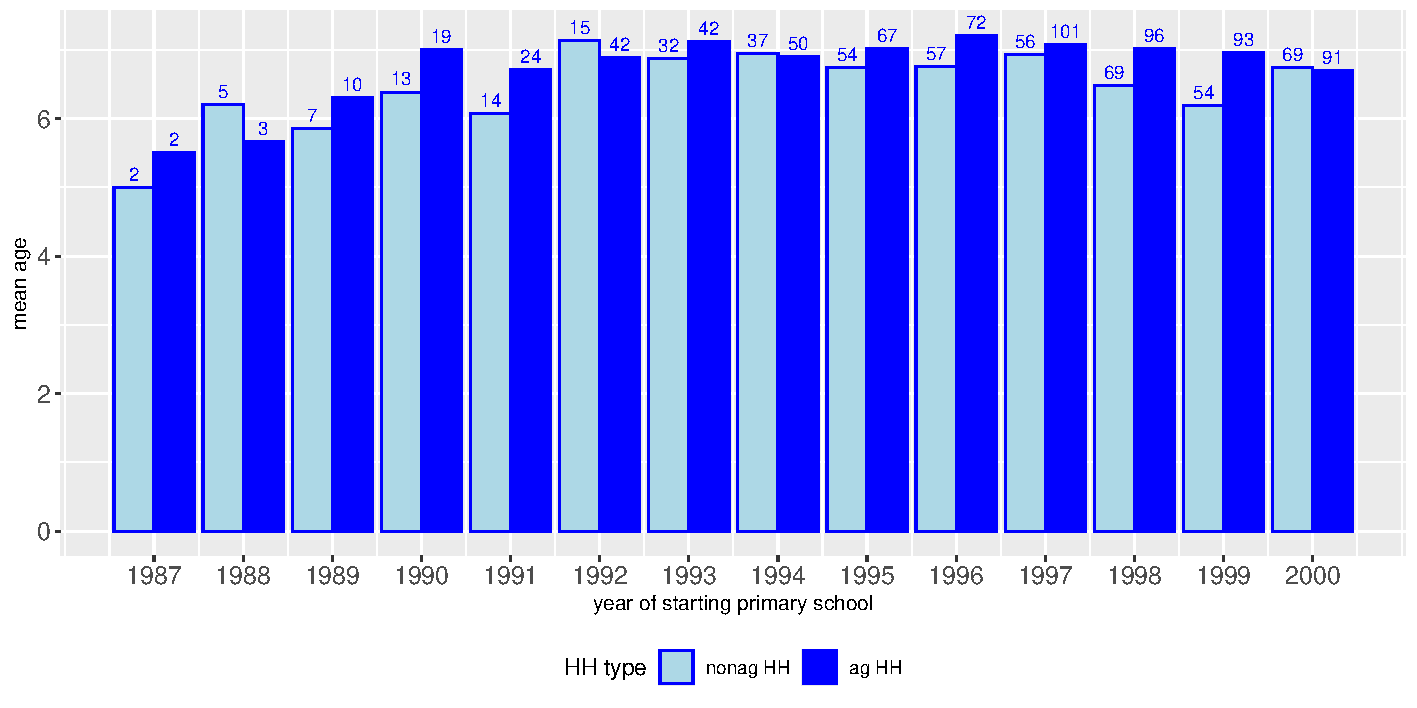
\includegraphics[width=.7\paperwidth]{AgeAtClass1Enrollment.pdf}\\
\renewcommand{\arraystretch}{1}
\hfil\begin{tabular}{>{\hfill\scriptsize}p{1cm}<{}>{\scriptsize}p{12cm}<{\hfill}}
Source:& Compiled from IFPRI data. All households, including attrited households, are used.\\[-1ex]
Notes:&: The Numbers displayed above the bar are cell sample size. \\[-1ex]
\end{tabular}
%\end{minipage}
\end{figure}

\textsc{\footnotesize Figure \ref{ERbyAge rawdata}} shows mean enrollment rates by age. Ages under primary and secondary schooling have less than 100\% enrollment rates. Age 5, one year before primary schooling begins, reports nonzero enrollment rates. These show that ``compulsory schooling'' is not enforced strictly. 

\textsc{\footnotesize Figure \ref{AgeAtClass1byAge rawdata}} shows the mean age of starting class 1 for each calendar year. Most years report the mean starting age older than six years old. This also shows that ``compulsory schooling'' is not enforced strictly. Agricultural households tend to start school later in age than non-agricultural households. This may partly explain why Agricultural households's enrollment rates are higher at some of the later ages. 


%\vspace{5.25cm}


%\begin{table}
%{\color{red}
%\hfil\textsc{\footnotesize Table \refstepcounter{table}\thetable: Main results by gender\label{MainGenderResults10Table}}\\
%\setlength{\tabcolsep}{1pt}
%\renewcommand{\arraystretch}{.75}
%\hfil\input{Tables/MainGenderResults10WithInteractionsTable.tex}
%\renewcommand{\arraystretch}{1}
%\hfil\begin{tabular}{>{\hfill\scriptsize}p{1cm}<{}>{\hfill\scriptsize}p{.25cm}<{}>{\scriptsize}p{.7\paperwidth}<{\hfill}}
%Source:& \multicolumn{2}{l}{\scriptsize Compiled from IFPRI data. }\\[-1ex]
%Notes:& 1. & Sample of direct offspring of household heads. \textsf{Agricultural households * year 2002} is an interaction term of agricultural household dummy and year 2002 dummy. All the interaction terms are demeaned. Columns \textsf{(1), (4), (7), (10)} use time-varying thana level characteristics (yield, mean rainfall, mean high temperature, mean low temperature), individual level characteristics (age squared, recipient of a poverty program), and \textsf{Demographic fixed trends} that are interactions of basline individual and demographic characterstics (sex of individual, household head's education, number of older male/female siblings) with year 2002 dummy $\bfx_{i}r_{t}$, and with year 2002 * agricultural household dummy $\bfx_{i}r_{t}D_{i}$. Columns \textsf{(2), (5), (8), (11)} add \textsf{other household fixed trends} that are interactions of other baseline household characteristics (per member land holding, per member nonland assets, own piped water, structured toilet). Columns \textsf{(3), (6), (9), (12)} add \textsf{Thana fixed trends} which allow heterogenous trends at Thana level. \\[-1ex]
%& 2. & Standard errors are clusterd at thana level. 95\% confidence intervals of cluster robust standard errors using Liang and Zeger are shown in parenthesis, bias-reduced linearization (Satterthwaite correction) for a correction of small number of clusters are shown in square brackets. $*$, $**$, $***$ indicate significance levels at 10\%, 5\%, 1\% under BRL cluster robust standard errors, respectively.\end{tabular}
%} % end of red ink
%\end{table}


%\begin{table}
%\hfil\textsc{\footnotesize Table \refstepcounter{table}\thetable: Main results by gender and by agricultural household definitions\label{MainGenderByAgdefResults}}\\
%\setlength{\tabcolsep}{1pt}
%\renewcommand{\arraystretch}{.75}
%\hspace{-1.0cm}\input{Tables/MainGenderByAgdefResults10WithInteractionsTable.tex}
%\end{table}


\pagebreak

%\newpage

\section{Additional Tables\label{app_a4}}

\begin{figure}[ht!]
\centering
\includegraphics[width = 11.5cm, height = 15cm]{Figures/Secondary School-Holiday-List-2019.jpg}\\
\caption{Government School Calendar in Bangladesh (2019).\footnote{Above is the Ministry of Education (MoE) Bangladesh provided examination and annual holiday calendar for the secondary and higher secondary schools (in Bangla). The bottom table of this notice contains the exam calendar, which instructed all the schools to hold annual exams from November 27 to December 11.}}
\label{school_calander_2019}
\end{figure}


\pagebreak

\begin{table}
\hfil\textsc{\footnotesize Table \refstepcounter{table}\thetable: Main results by gender and by agricultural household definitions\label{MainGenderByAgdefResults}}\\
\setlength{\tabcolsep}{1pt}
\renewcommand{\arraystretch}{.75}
\hspace{-1.0cm}\input{Tables/MainGenderByAgdefResults10WithInteractionsTable.tex}
\renewcommand{\arraystretch}{1}
\hfil\begin{tabular}{>{\hfill\scriptsize}p{1cm}<{}>{\hfill\scriptsize}p{.25cm}<{}>{\scriptsize}p{.7\paperwidth}<{\hfill}}
Source:& \multicolumn{2}{l}{\scriptsize Compiled from IFPRI data. }\\[-1ex]
Notes:& 1. & Sample of direct offspring of household heads. \textsf{AgriHH * year 2002} is an interaction term of agricultural household dummy and year 2002 dummy. All the interaction terms are demeaned. Specification 1 uses time-varying thana level characteristics (yield, mean rainfall, mean high temperature, mean low temperature), individual-level characteristics (age squared, recipient of a poverty program), and \textsf{Demographic fixed trends} that are interactions of baseline individual and demographic characteristics (sex of individual, household head's education, number of older male/female siblings) with the year 2002 dummy, and sex of individual with the year 2002 * agricultural household dummy. Parental education is highly collinear with agricultural household dummy and is dropped from triple interactions. Specification 2 add \textsf{other household fixed trends} that are interactions of other baseline household characteristics (per member land holding, per member non-land assets, own piped water, structured toilet). Specification 3 adds \textsf{Thana fixed trends}, which allow heterogeneous trends at the Thana level. \\[-1ex]
& 2. & Standard errors are clustered at thana level. 95\% confidence intervals of cluster robust standard errors using \cite{liang1986longitudinal} are shown in parenthesis, and bias-reduced linearization (Satterthwaite correction) for a correction of a small number of clusters are shown in square brackets. $*$, $**$, $***$ indicate significance levels at 10\%, 5\%, 1\% under BRL cluster robust standard errors, respectively.\end{tabular}
\end{table}


\begin{table}
\hfil\textsc{\footnotesize Table \refstepcounter{table}\thetable: Main results by gender and by age lower-bound definitions\label{MainByGenderByAgeLBAgHH0Results}}\\
\setlength{\tabcolsep}{1pt}
\renewcommand{\arraystretch}{.75}
\hspace{-1.0cm}\input{Tables/MainByGenderByAgeLBAgHH0Results.tex}\\
\renewcommand{\arraystretch}{1}
\hfil\begin{tabular}{>{\hfill\scriptsize}p{1cm}<{}>{\hfill\scriptsize}p{.25cm}<{}>{\scriptsize}p{.7\paperwidth}<{\hfill}}
Source:& \multicolumn{2}{l}{\scriptsize Compiled from IFPRI data. }\\[-1ex]
Notes:& 1. & Sample of direct offspring of household heads. \textsf{AgriHH * year 2002} is an interaction term of agricultural household dummy and year 2002 dummy. All the interaction terms are demeaned. Specification 1 uses time-varying thana level characteristics (yield, mean rainfall, mean high temperature, mean low temperature), individual-level characteristics (age squared, recipient of a poverty program), and \textsf{Demographic fixed trends} that are interactions of baseline individual and demographic characteristics (sex of individual, household head's education, number of older male/female siblings) with the year 2002 dummy, and sex of individual with the year 2002 * agricultural household dummy. Parental education is highly collinear with agricultural household dummy and is dropped from triple interactions.  Specification 2 add \textsf{other household fixed trends} that are interactions of other baseline household characteristics (per member land holding, per member non-land assets, own piped water, structured toilet). Specification 3 adds \textsf{Thana fixed trends}, which allow heterogeneous trends at the Thana level. \\[-1ex]
& 2. & Standard errors are clustered at thana level. 95\% confidence intervals of cluster robust standard errors using \cite{liang1986longitudinal} are shown in parenthesis, and bias-reduced linearization (Satterthwaite correction) for a correction of a small number of clusters are shown in square brackets. $*$, $**$, $***$ indicate significance levels at 10\%, 5\%, 1\% under BRL cluster robust standard errors, respectively.\end{tabular}
\end{table}

\begin{table}
\hfil\textsc{\footnotesize Table \refstepcounter{table}\thetable: Main results by gender and age group\label{MainGenderAgeGroup2ResultsWithInteractions}}\\
\setlength{\tabcolsep}{1pt}
\renewcommand{\arraystretch}{.55}
\hspace{-1cm}\input{Tables/MainGenderAgeGroup2ResultsWithInteractions.tex}

\renewcommand{\arraystretch}{1}
\hfil\begin{tabular}{>{\hfill\scriptsize}p{1cm}<{}>{\hfill\scriptsize}p{.5cm}<{}>{\scriptsize}p{12cm}<{\hfill}}
Source:& \multicolumn{2}{l}{\scriptsize Compiled from IFPRI data. }\\[-1ex]
Notes:& 1. & Sample of direct offspring of household heads. \textsf{Agricultural households * year 2002} is an interaction term of agricultural household dummy and year 2002 dummy. All the interaction terms are demeaned. Columns \textsf{(1), (4), (7), (10)} use time-varying thana level characteristics (yield, mean rainfall, mean high temperature, mean low temperature), individual-level characteristics (age squared, recipient of a poverty program), and \textsf{Demographic fixed trends} that are interactions of baseline individual and demographic characteristics (sex of individual, household head's education, number of older male/female siblings) with year 2002 dummy $\bfx_{i}r_{t}$, and with year 2002 * agricultural household dummy $\bfx_{i}r_{t}D_{i}$. Parental education is highly collinear with agricultural household dummy and is dropped from triple interactions. Columns \textsf{(2), (5), (8), (11)} add \textsf{Other household fixed trends} that are interactions of other baseline household characteristics (per member land holding, per member non-land assets, own piped water, structured toilet). Columns \textsf{(3), (6), (9), (12)} add \textsf{Thana fixed trends}, which allow heterogeneous trends at the Thana level. \\[-1ex]
& 2. & Standard errors are clustered at thana level. 95\% confidence intervals of cluster robust standard errors using \citep{liang1986longitudinal} are shown in parenthesis, bias-reduced linearization (Satterthwaite correction) for a correction of a small number of clusters are shown in square brackets. $*$, $**$, $***$ indicate significance levels at 10\%, 5\%, 1\% under BRL cluster robust standard errors, respectively.
\end{tabular}
\end{table}



\begin{table}
\hfil\textsc{\footnotesize Table \refstepcounter{table}\thetable: Placebo test results by gender\label{PlaceboResults10Table}}\\
\setlength{\tabcolsep}{1pt}
\renewcommand{\arraystretch}{.75}
\hfil\input{Tables/Placebo10agHH0ByGenderWithInteractionsResults.tex}

\renewcommand{\arraystretch}{1}
\hfil\begin{tabular}{>{\hfill\scriptsize}p{1cm}<{}>{\hfill\scriptsize}p{.25cm}<{}>{\scriptsize}p{.7\paperwidth}<{\hfill}}
Source:& \multicolumn{2}{l}{\scriptsize Compiled from IFPRI data. }\\[-1ex]
Notes:& 1. & Sample of direct offspring of household heads. \textsf{Agricultural households * year 2002} is an interaction term of agricultural household dummy and year 2002 dummy. All the interaction terms are demeaned. Columns \textsf{(1), (4)} use time-varying thana-level characteristics (yield, mean rainfall, mean high temperature, mean low temperature), individual-level characteristics (age squared, recipient of a poverty program), and \textsf{Demographic fixed trends} that are interactions of baseline individual and demographic characteristics (sex of individual, household head's education, number of older male/female siblings) with the year 2002 dummy, and sex of individual with the year 2002 * agricultural household dummy. Parental education is highly collinear with agricultural household dummy and is dropped from triple interactions. Columns \textsf{(2), (5)} add \textsf{other household fixed trends} that are interactions of other baseline household characteristics (per member land holding, per member non-land assets, own piped water, structured toilet). Columns \textsf{(3), (6)} add \textsf{Thana fixed trends}, which allow heterogeneous trends at the Thana level. \\[-1ex]
& 2. & Standard errors are clustered at thana level. 95\% confidence intervals of cluster robust standard errors using \cite{liang1986longitudinal} are shown in parenthesis, and bias-reduced linearization (Satterthwaite correction) for a correction of the small number of clusters are shown in square brackets. $*$, $**$, $***$ indicate significance levels at 10\%, 5\%, 1\% under BRL cluster robust standard errors, respectively. \end{tabular}
\end{table}



%\begin{table}[bp]
%\caption{Tabulation of Enrollment against Program support using first round of data collected in 1999}
%\label{enrollprogram}
%\begin{center}
%{
%\resizebox{12.5cm}{!}{
%\begin{tabular}{lccccccc}
%\hline
%School              & No Program            & FFW   & IFS-FFA   & Primary           & RMP   & Secondary         & VGD        \\
%enrollment          & support               &       &           & stipend           &       & stipend           &            \\
%\hline
%Yes                 & 7                     & 180   & 5         & 190               & 164   & 187               & 109        \\
%No                  & 329                   & 2     & 0         & 1                 & 0     & 0                 & 0          \\
%\hline
%\hline
%\multicolumn{8}{p{22cm}}{{\footnotesize Notes: Compiled for those who are aged $6 - 21$ in 1999. Abbreviations used for programs are the following: FFW (Food-For-Work), IFS-FFA (Integrated Food Security - Food For Asset Creation), RMP (Rural Maintenance Program) , VGD (Vulnerable Group Development). Enrollment information is asked in 1999, which is before the end of school year 1999. Program Support information is that of 1999.}}
%\end{tabular}}}
%\end{center}
%\end{table}



%\begin{table}[bp]
%\caption{Tabulation of Agricultural vs. Non-Agriculture household enrollment, age cohort (10-18 years old in 1999)}
%\label{schooling1}
%\begin{center}
%{
%\resizebox{5.5cm}{!}{
%\begin{tabular}{lcc}
%\hline
%\hline
%School Enrollment                           & 1999 & 2002 \\
%\hline
%Agricultural                                & 0.732 & 0.391\\
%Non-agricultural                            & 0.728 & 0.458\\
%Difference-in-Difference                    & -0.72** &     \\
%\hline
%\end{tabular}}}
%\end{center}
%\end{table}

\pagebreak



%\begin{figure}[h!]
%\centering
%\includegraphics[width = 11.5cm, height = %15cm]{Secondary-School-Holiday-List-2020.jpg}\\
%\caption{Government School Calendar in Bangladesh (2020).\footnote{This is the Education Ministry of Bangladesh provided examination and annual holiday calendar for the primary schools (in Bangla). The second table of this notice contains the exam calendar. The notice instructed all the schools to hold annual exams from 28th November to 10th December, 2020.}}
%\label{school_calander_2020}
%\end{figure}



\begin{table}[t]
\caption{Descriptive Statistics: HIES (2016) with 10-27 years old in 1999 }
\label{tab_destat_6:hies}
\begin{center}
{
\resizebox{13.5cm}{!}{
\begin{tabular}{lcccc}
\hline
Variables                           & Mean          & STD       & Max       & Min        \\
\hline
Income (in taka) &   12562.64 &   14940.05 &     480000 &          0 \\
Years of education  &   4.634214 &   4.560333 &         18 &          0 \\
Education completed: Primary &   0.505697 &   0.499971 &          1 &          0 \\
Education completed: Secondary &   0.293591 &    0.45541 &          1 &          0 \\
Education completed: Higher Secondary &   0.155453 &   0.362339 &          1 &          0 \\
Age (in years) &   37.41189 &   7.633799 &         52 &         26 \\
Gender: Male &    0.48575 &   0.499801 &          1 &          0 \\
Residency: Rural &   0.683457 &   0.465131 &          1 &          0 \\
Religion: Muslim        &   0.859788 &   0.347209 &          1 &          0 \\
\hline
No. of Observation      &   66,528   &            &            &            \\            
\hline
%Area under agriculture underproduction &   33.38&       16.71&           9&          90            \\
%Rainfall2004                       &      103.69&       54.19&          41&         291            \\
%Rice                               &     4552.29&     4156.40&          14&       14885            \\
%Wheat                              &     5331.90&     7333.49&           0&       22514            \\
%Maize                              &      905.93&      759.93&           0&        2512            \\
\hline
\multicolumn{5}{p{15cm}}{{\footnotesize Notes: All information is based on the HIES (2016) data-set. STD represents Standard deviation.}}
\end{tabular}}}
\end{center}
\end{table}

\begin{table}[t]
\caption{Cohort Analysis Data on Bangladesh: HIES (2016)}
\label{tab_destat_3}
\begin{center}
{
\resizebox{8.5cm}{!}{
    \begin{tabular}{cc}
          &  \\
    \midrule
    Age Classification & Number of Observation  \\
    \midrule
    Cohort 1 (Age 10-18 in 1999) & 26100 \\
    \midrule
    Age 10 in 1999 & 3,387 \\
    Age 11 in 1999 & 2,650 \\
    Age 12 in 1999 & 3,929 \\
    Age 13 in 1999 & 1,978 \\
    Age 14 in 1999 & 4,533 \\
    Age 15 in 1999 & 2,068 \\
    Age 16 in 1999 & 3,754 \\
    Age 17 in 1999 & 1,889 \\
    Age 18 in 1999 & 1,912 \\
    \midrule
    Cohort 2 (Age 19-27 in 1999) & 23120 \\
    \midrule
    Age 19 in 1999 & 4,944 \\
    Age 20 in 1999 & 2,974 \\
    Age 21 in 1999 & 1,841 \\
    Age 22 in 1999 & 2,698 \\
    Age 23 in 1999 & 1,416 \\
    Age 24 in 1999 & 3,676 \\
    Age 25 in 1999 & 1,619 \\
    Age 26 in 1999 & 2,577 \\
    Age 27 in 1999 & 1,375 \\
    \midrule
          &  \\
\end{tabular}}}
\end{center}
\end{table}



%\vspace{0.5cm}
\begin{table}[h!]
\caption{\textbf{Cohort Analysis 2: (Aged 10-27 in 2016)}}
\label{cohort2}
\begin{center}
{
\resizebox{11.5cm}{!}{
\begin{tabular}{lcccc}
    \toprule
\textbf{Variables}                          & \textbf{Years of }    & \textbf{Primary}  & \textbf{Secondary}  & \textbf{Higher}  \\
                                            &\textbf{Education}    &                   &                     & \textbf{Secondary} \\
\cmidrule{2-5}
\textbf{Estimation: } & \multicolumn{1}{c}{\textbf{OLS}} & \multicolumn{3}{c}{\textbf{Probit}}\\
\cmidrule(lr){2-2}\cmidrule(lr){3-5}
\multicolumn{1}{c}{}                        & (1)                   & (2)               & (3)                   & (4)          \\
\hline
(Aged 10 in 1999) X (Rural)             & 1.067***              &       0.368***    &       0.370***        &       0.296** \\
                                        &     (0.343)           &     (0.108)       &     (0.108)           &     (0.120)         \\
[1em]
(Aged 11 in 1999) X (Rural)            &       0.873**          &       0.213*      &       0.230**         &       0.330***  \\
                                        &     (0.412)           &     (0.119)        &     (0.117)         &     (0.123)         \\
[1em]
(Aged 12 in 1999) X (Rural)            &        0.910**         &       0.278***    &       0.283***        &       0.345***\\
                                        &     (0.366)           &     (0.101)         &     (0.106)         &     (0.128)         \\
[1em]
(Aged 13 in 1999) X (Rural)             &       0.933*          &       0.335**         &       0.351***    &       0.230         \\
                                        &     (0.487)           &     (0.138)         &     (0.131)         &     (0.150)         \\
[1em]
(Aged 14 in 1999) X (Rural)             &       1.339***        &       0.360***    &       0.364***        &       0.371***    \\
                                        &     (0.357)           &    (0.0979)         &     (0.106)         &     (0.116)         \\
[1em]
(Aged 15 in 1999) X (Rural)             &       0.897**         &       0.228**     &       0.233*          &       0.257*      \\
                                        &     (0.386)         &     (0.110)         &     (0.133)           &     (0.132)         \\
[1em]
(Aged 16 in 1999) X (Rural)             &       0.261         &       0.116         &       0.147         &       0.218*        \\
                                        &     (0.391)         &     (0.117)         &     (0.117)         &     (0.125)         \\
[1em]
(Aged 17 in 1999) X (Rural)             &       0.417         &      0.0876         &       0.184         &       0.272*        \\
                                        &     (0.443)         &     (0.127)         &     (0.117)         &     (0.139)         \\
[1em]
(Aged 18 in 1999) X (Rural)             &       0.416         &      0.0561         &       0.182         &       0.241*        \\
                                        &     (0.406)         &     (0.121)         &     (0.123)         &     (0.146)         \\
\hline
Other Control                           &    Yes            &  Yes                  &   Yes                 &   Yes       \\
District Control                        &    Yes            &  Yes                  &   Yes                 &   Yes       \\
District \times \textnormal{Age Control}                            &    Yes    &  Yes      &   Yes         &   Yes       \\
Observations                            &       49165         &       49129         &       49128           &       48987         \\
\hline
\hline\\
\multicolumn{5}{p{15cm}}{{\footnotesize Source: Compiled from HIES 2016 data.
Notes: 1. Regression estimated using OLS with standard errors clustered at \textit{district} level reported in the parenthesis. $*$, $**$, $***$ indicate significance levels at 10\%, 5\%, 1\%, respectively.
2. Regression estimates control for the cohort of birth dummy, sex, type of location (rural or urban), district and cohort of birth dummy interactions, and religion.}}.
\end{tabular}}}
\end{center}
\end{table}


\begin{table}[h!]
\caption{\textbf{common trend test with HIES 2016: (Aged 19-27 in 1999)}}
\label{cohort4}
\begin{center}
{
\resizebox{12.5cm}{!}{
\begin{tabular}{lcccc}
    \toprule
\textbf{Variables}                          & \textbf{Years of }    & \textbf{Primary}  & \textbf{Secondary}  & \textbf{Higher}  \\
                                            &\textbf{Education}    &                   &                     & \textbf{Secondary} \\
\cmidrule{2-5}
\textbf{Estimation: } & \multicolumn{1}{c}{\textbf{OLS}} & \multicolumn{3}{c}{\textbf{Probit}}\\
\cmidrule(lr){2-2}\cmidrule(lr){3-5}
\multicolumn{1}{c}{}                        & (1)                   & (2)               & (3)                   & (4)          \\
\hline
%{\textbf{Panel A:  }}                        &                       &                   &                       &               \\
%Aged 6-18 in 1999                           &       1.665***        &       0.193***    &       0.121***        &      0.0589***\\
%                                           &    (0.0598)         &   (0.00712)         &   (0.00478)         &   (0.00426)         \\
%\textbf{Panel A}                            &                       &                   &                       &                   \\
%Aged 20-27 in 1999                          & -1.025***             & -0.262***         & -0.0986**             & -0.380***         \\
%                                            & (0.13)                & (0.04)            & (0.04)                & (0.04)            \\
%(Aged 20-27 in 1999) X (Rural)              & -0.0281               & -0.00868          & -0.0267               & -0.0894           \\
%                                            & (0.19)                & (0.05)            & (0.06)                & (0.06)            \\
%\textbf{Panel B}                            &                       &                   &                       &                   \\
(Aged 20 in 1999) X (Rural)                 & 0.395                 & 0.0924            & 0.0722                & -0.0198           \\
                                            & (0.26)                & (0.07)            & (0.08)                & (0.09)            \\
(Aged 21 in 1999) X (Rural)                 & -0.189                & 0.0623            & -0.0514               &  -0.210**         \\
                                            & (0.31)                & (0.08)            & (0.08)                & (0.09)            \\
(Aged 22 in 1999) X (Rural)                 & -0.349                &  -0.184**         & -0.0539               & -0.0289           \\
                                            & (0.30)                & (0.08)            & (0.09)                & (0.09)            \\
(Aged 23 in 1999) X (Rural)                 & -0.181                & -0.0822           & -0.0223               & -0.121            \\
                                            & (0.37)                & (0.10)            & (0.11)                & (0.12)            \\
(Aged 24 in 1999) X (Rural)                 & 0.131                 & 0.0214            & -0.0387               & -0.078            \\
                                            & (0.24)                & (0.06)            & (0.07)                & (0.07)            \\
(Aged 25 in 1999) X (Rural)                 & 0.133                 & 0.0177            & -0.0272               & 0.0177            \\
                                            & (0.34)                & (0.09)            & (0.11)                & (0.11)            \\
(Aged 26 in 1999) X (Rural)                 & -0.136                & 0.0198            & -0.0374               &  -0.161*          \\
                                            & (0.29)                & (0.07)            & (0.09)                & (0.09)            \\
(Aged 27 in 1999) X (Rural)                 & -0.364                & -0.0928           & -0.122                &  -0.213*          \\
                                            & (0.38)                & (0.10)            & (0.11)                & (0.12)            \\
\hline
P-value for joint significance    &                       &                   &                       &                   \\
test for age and rural interaction terms    & 0.39                  & 0.13              & 0.54                  & 0.25              \\
\hline
Other Control                               &    Yes            &  Yes      &   Yes     &   Yes       \\
District Control                            &    Yes            &  Yes      &   Yes     &   Yes       \\
District \times \textnormal{Age Control}    &    Yes            &  Yes      &   Yes     &   Yes       \\
Observations                                &  23100            & 23087     & 23063     & 22986       \\
\hline
\hline\\
\multicolumn{5}{p{17cm}}{{\footnotesize Source: Compiled from HIES 2016 data.
Notes: 1. Standard errors clustered at \textit{district} level reported in the parenthesis. $*$, $**$, $***$ indicate significance levels at 10\%, 5\%, 1\%, respectively.
2. Regression estimates control for cohort of birth dummy, sex, district and cohort of birth dummy interactions, and religion.}}.
\end{tabular}}}
\end{center}
\end{table}


\begin{table}[h!]
\caption{\textbf{Education Return: Dependent variable:  log of income}}
\label{mincer}
\begin{center}
{
\resizebox{11.5cm}{!}{
\begin{tabular}{lc}
    \toprule
\textbf{Variables}                          & \textbf{Co-efficient}   \\
\hline
Years of education                              &      0.0663***\\
                                                &   (0.00356)         \\
[1em]
Age                                             &      0.0313         \\
                                                &    (0.0280)         \\
[1em]
Age Squared                                     &   -0.000280         \\
                                                &  (0.000412)         \\
[1em]
Male                                            &       0.525***\\
                                                &    (0.0412)         \\
[1em]
Rural                                           &     -0.0640** \\
                                                &    (0.0315)         \\
[1em]
Muslim                                          &      0.0611         \\
                                                &    (0.0388)         \\

\hline
District Control                                &    Yes           \\
Observations                                    &       6698      \\
\hline\\
\multicolumn{2}{p{15cm}}{{\footnotesize Source: Compiled from HIES 2016 data.
Notes: Regression estimated using OLS with standard errors clustered at \textit{district} level reported in the parenthesis. $*$, $**$, $***$ indicate significance levels at 10\%, 5\%, 1\%, respectively.}}.
\end{tabular}}}
\end{center}
\end{table}


\begin{table}[t]
\caption{India State Wide Academic and Agricultural Calendar}
\label{india3}
\begin{center}
{
\resizebox{18.5cm}{!}{
\begin{tabular}{lccccccc}
\hline
{\bf States} & {\bf Major Crop } & {\bf Area under crop}    & {\bf Academic Session} & {\bf Final Exam} & {\bf Harvest Period} & {\bf Final Exam timing } \\
{\bf } &                  & {\bf (\% of cropped area)} & {\bf } & {\bf } & {\bf of major crop} & {\bf overlaps with} \\
{\bf } &                  & {\bf } & {\bf } & {\bf } & {\bf  } & {\bf Harvesting period} \\
\hline
Andhra Pradesh &      Rice  &       30\% & June to April &  April/May & November December &         No \\
Arunachal Pradesh &       Rice &       47\% & July to April &   February & November-December &         No \\
Assam &       Rice &       62\% & January to December &   December & November December &        Yes \\
Bihar &       Rice &       44\% & April to March &      March & September to November &         No \\
%Chhattisgarh &       Rice &       69\% & June to April & March-April & October to November &         No \\
%\hline
Delhi &      Wheat &       45\% & April to March &      March & March-April &        Yes \\
Goa &       Rice &       29\% & June to April &      March & September-October &         No \\
Gujarat &     Cotton &       23\% & June to May &      March & October to April &        Yes \\
Haryana &      Wheat &       39\% & April to March &  Feb-March &  April-May &         No \\
Himachal Pradesh &      Wheat &       38\% & April to March &      March & April-June &         No \\
Jammu-Kashmir &      Wheat &       26\% & November to October & October-November & April-June &         No \\
Jharkhand &       Rice &       69\% & April to June & January-March & September to November &         No \\
Karnataka &      Pulse &       18\% & May to April &      March & November-January &         No \\
Kerala &       Rice &        8\% & June to March &      March & September-October &         No \\
Madhya Pradesh &      Wheat &       23\% & July to April &      March & February-April &        Yes \\
Maharashtra &     Cotton &       19\% & June to May &      March &    Nov-Jan &         No \\
Manipur &       Rice &       61\% & Feb to Jan & December-January & October-November &         No \\
Meghalaya &       Rice &       32\% & Feb to Jan &   October  & October-December &        Yes \\
Mizoram &       Rice &       26\% & Jan to Dec & November-December & October-December &        Yes \\
Nagaland &       Rice &       38\% & Jan to Dec & November-December & September-November &        Yes \\
Odisha &       Rice &       83\% & April to March &      March & September-October &         No \\
Puducherry &       Rice &       63\% & June to April & March-April & September-October &         No \\
Punjab &      Wheat &       45\% & April to March &      March &  April-May &         No \\
Rajasthan &      Pulse &       16\% & July to June &      March &  Feb-March &        Yes \\
 % Sikkim &       Rice &        9\% & Feb to December & November-December & September-November &        Yes \\
%\hline
Tamil Nadu &       Rice &       33\% & June to April & March-April & September-October &         No \\
Tripura &       Rice &       53\% & Jan to Dec & November-December & September-November &        Yes \\
Uttar Pradesh &      Wheat &       38\% & July to June & February-March & March-April &        Yes \\
Uttarakhand &      Wheat &       31\% & April to March & March-April & March-April &        Yes \\
West Bengal &       Rice &       58\% & Feb to Dec & November-December & August-November &        Yes \\
\hline
\end{tabular}}}
\end{center}
\end{table}

\begin{table}[t]
\caption{Descriptive Statistics: India sample (2004)}
\label{tab_destat_5}
\begin{center}
{
\resizebox{10.5cm}{!}{
\begin{tabular}{lcccc}
\hline
Variables                           & Mean          & STD       & Max       & Min                   \\
\hline
Enrolled                            &        1.00&        0.00&           1&           1            \\
Completed Years of education        &        2.82&        2.18&           0&          12            \\
Agricultural Households             &    0.385   & 0.485      &  0         &        1               \\
Overlapping State                   &    0.352   & 0.477      &  0         &           1            \\
Age                                 &        9.10&        2.38&           5&          13            \\
Mother's Age                        &       33.95&        6.32&          18&          80            \\
Father's Age                        &       38.79&        7.03&          21&          88            \\
Father's Education                  &        2.15&        3.43&           0&          15            \\
Mother's Education                  &        4.44&        4.44&           0&          16            \\
No. of Assets                       &        8.78&        4.55&           0&          25            \\
Household Size                      &        6.67&        2.72&           2&          38            \\
%Area under agriculture underproduction &   33.38&       16.71&           9&          90            \\
%Rainfall2004                       &      103.69&       54.19&          41&         291            \\
%Rice                               &     4552.29&     4156.40&          14&       14885            \\
%Wheat                              &     5331.90&     7333.49&           0&       22514            \\
%Maize                              &      905.93&      759.93&           0&        2512            \\
\hline
No. of Observation                  &   24378   &            &            &                         \\   
\hline
\multicolumn{5}{p{10cm}}{{\footnotesize Notes: All information is based on the first round of the data set, which was collected in 2004. Agricultural household is an indicator variable for a household whose primary income is agriculture. Agricultural household (head) is defined as head is claiming that main income source is agriculture. STD represents Standard deviation.}}
\end{tabular}}}
\end{center}
\end{table}

\end{document}


https://www.overleaf.com/project/62d977da936e6a331c7685e1